
% Options for packages loaded elsewhere
\PassOptionsToPackage{unicode}{hyperref}
\PassOptionsToPackage{hyphens}{url}
\documentclass[
]{article}
\usepackage[left=2cm,right=2cm,top=2cm,bottom=2cm]{geometry}
\usepackage{pdflscape}
\usepackage{xcolor}
\usepackage{amsmath,amssymb}
\usepackage{float}
\setcounter{secnumdepth}{3}
\usepackage{graphicx}
\usepackage{iftex}
\ifPDFTeX
  \usepackage[T1]{fontenc}
  \usepackage[utf8]{inputenc}
  \usepackage{textcomp} % provide euro and other symbols
\else % if luatex or xetex
  \usepackage{unicode-math} % this also loads fontspec
  \defaultfontfeatures{Scale=MatchLowercase}
  \defaultfontfeatures[\rmfamily]{Ligatures=TeX,Scale=1}
\fi
\usepackage{lmodern}
\ifPDFTeX\else
  % xetex/luatex font selection
\fi
% Use upquote if available, for straight quotes in verbatim environments
\IfFileExists{upquote.sty}{\usepackage{upquote}}{}
\IfFileExists{microtype.sty}{% use microtype if available
  \usepackage[]{microtype}
  \UseMicrotypeSet[protrusion]{basicmath} % disable protrusion for tt fonts
}{}
\makeatletter
\@ifundefined{KOMAClassName}{% if non-KOMA class
  \IfFileExists{parskip.sty}{%
    \usepackage{parskip}
  }{% else
    \setlength{\parindent}{0pt}
    \setlength{\parskip}{6pt plus 2pt minus 1pt}}
}{% if KOMA class
  \KOMAoptions{parskip=half}}
\makeatother
\usepackage{color}
\usepackage{fancyvrb}
\newcommand{\VerbBar}{|}
\newcommand{\VERB}{\Verb[commandchars=\\\{\}]}
\DefineVerbatimEnvironment{Highlighting}{Verbatim}{commandchars=\\\{\}}
% Add ',fontsize=\small' for more characters per line
\newenvironment{Shaded}{}{}
\newcommand{\AlertTok}[1]{\textcolor[rgb]{1.00,0.00,0.00}{\textbf{#1}}}
\newcommand{\AnnotationTok}[1]{\textcolor[rgb]{0.38,0.63,0.69}{\textbf{\textit{#1}}}}
\newcommand{\AttributeTok}[1]{\textcolor[rgb]{0.49,0.56,0.16}{#1}}
\newcommand{\BaseNTok}[1]{\textcolor[rgb]{0.25,0.63,0.44}{#1}}
\newcommand{\BuiltInTok}[1]{\textcolor[rgb]{0.00,0.50,0.00}{#1}}
\newcommand{\CharTok}[1]{\textcolor[rgb]{0.25,0.44,0.63}{#1}}
\newcommand{\CommentTok}[1]{\textcolor[rgb]{0.38,0.63,0.69}{\textit{#1}}}
\newcommand{\CommentVarTok}[1]{\textcolor[rgb]{0.38,0.63,0.69}{\textbf{\textit{#1}}}}
\newcommand{\ConstantTok}[1]{\textcolor[rgb]{0.53,0.00,0.00}{#1}}
\newcommand{\ControlFlowTok}[1]{\textcolor[rgb]{0.00,0.44,0.13}{\textbf{#1}}}
\newcommand{\DataTypeTok}[1]{\textcolor[rgb]{0.56,0.13,0.00}{#1}}
\newcommand{\DecValTok}[1]{\textcolor[rgb]{0.25,0.63,0.44}{#1}}
\newcommand{\DocumentationTok}[1]{\textcolor[rgb]{0.73,0.13,0.13}{\textit{#1}}}
\newcommand{\ErrorTok}[1]{\textcolor[rgb]{1.00,0.00,0.00}{\textbf{#1}}}
\newcommand{\ExtensionTok}[1]{#1}
\newcommand{\FloatTok}[1]{\textcolor[rgb]{0.25,0.63,0.44}{#1}}
\newcommand{\FunctionTok}[1]{\textcolor[rgb]{0.02,0.16,0.49}{#1}}
\newcommand{\ImportTok}[1]{\textcolor[rgb]{0.00,0.50,0.00}{\textbf{#1}}}
\newcommand{\InformationTok}[1]{\textcolor[rgb]{0.38,0.63,0.69}{\textbf{\textit{#1}}}}
\newcommand{\KeywordTok}[1]{\textcolor[rgb]{0.00,0.44,0.13}{\textbf{#1}}}
\newcommand{\NormalTok}[1]{#1}
\newcommand{\OperatorTok}[1]{\textcolor[rgb]{0.40,0.40,0.40}{#1}}
\newcommand{\OtherTok}[1]{\textcolor[rgb]{0.00,0.44,0.13}{#1}}
\newcommand{\PreprocessorTok}[1]{\textcolor[rgb]{0.74,0.48,0.00}{#1}}
\newcommand{\RegionMarkerTok}[1]{#1}
\newcommand{\SpecialCharTok}[1]{\textcolor[rgb]{0.25,0.44,0.63}{#1}}
\newcommand{\SpecialStringTok}[1]{\textcolor[rgb]{0.73,0.40,0.53}{#1}}
\newcommand{\StringTok}[1]{\textcolor[rgb]{0.25,0.44,0.63}{#1}}
\newcommand{\VariableTok}[1]{\textcolor[rgb]{0.10,0.09,0.49}{#1}}
\newcommand{\VerbatimStringTok}[1]{\textcolor[rgb]{0.25,0.44,0.63}{#1}}
\newcommand{\WarningTok}[1]{\textcolor[rgb]{0.38,0.63,0.69}{\textbf{\textit{#1}}}}
\usepackage{longtable,booktabs,array}
\newcounter{none} % for unnumbered tables
\usepackage{calc} % for calculating minipage widths
% Correct order of tables after \paragraph or \subparagraph
\usepackage{etoolbox}
\makeatletter
\patchcmd\longtable{\par}{\if@noskipsec\mbox{}\fi\par}{}{}
\makeatother
% Allow footnotes in longtable head/foot
\IfFileExists{footnotehyper.sty}{\usepackage{footnotehyper}}{\usepackage{footnote}}
\makesavenoteenv{longtable}
\usepackage{graphicx}
\makeatletter
\newsavebox\pandoc@box
\newcommand*\pandocbounded[1]{% scales image to fit in text height/width
  \sbox\pandoc@box{#1}%
  \Gscale@div\@tempa{\textheight}{\dimexpr\ht\pandoc@box+\dp\pandoc@box\relax}%
  \Gscale@div\@tempb{\linewidth}{\wd\pandoc@box}%
  \ifdim\@tempb\p@<\@tempa\p@\let\@tempa\@tempb\fi% select the smaller of both
  \ifdim\@tempa\p@<\p@\scalebox{\@tempa}{\usebox\pandoc@box}%
  \else\usebox{\pandoc@box}%
  \fi%
}
% Set default figure placement to htbp
\def\fps@figure{htbp}
\makeatother
\setlength{\emergencystretch}{3em} % prevent overfull lines
\providecommand{\tightlist}{%
  \setlength{\itemsep}{0pt}\setlength{\parskip}{0pt}}
\usepackage{bookmark}
\IfFileExists{xurl.sty}{\usepackage{xurl}}{} % add URL line breaks if available
\urlstyle{same}
\hypersetup{
  hidelinks,
  pdfcreator={LaTeX via pandoc}}

\author{}
\date{}

\begin{document}

\begin{center}
    {\LARGE\textbf{Week 8 Report}}\\[0.5em]
    {\LARGE\textbf{3D Printer Production Simulator}}\\[0.7em]
    {\normalsize Pol Plana · Alba Roma · Emma Nájera}
\end{center}

\vspace{1em}

\section{System Architecture}\label{a-system-architecture}

The completed system consists of three independent services: provider, manufacturer, and retailer, plus a turn engine that
orchestrates them through simulated time. Each service owns its own
SQLite database and its own day counter. No service reads another's
database. All cross-service communication goes through HTTP/JSON over
documented REST contracts.

The full system architecture diagram is shown in Appendix~\ref{appendix:architecture}.

\subsection{Turn Engine: Order of
Operations}\label{turn-engine-order-of-operations}

Each simulated day runs in five phases:

\begin{enumerate}
\def\labelenumi{\arabic{enumi}.}
\tightlist
\item
  \textbf{Signal injection.} The engine reads the active scenario event
  for the current day and applies the \texttt{supply\_modifier} and
  \texttt{lead\_time\_modifier} to the provider's stock replenishment
  settings.
\item
  \textbf{Demand injection.} The engine generates synthetic customer
  orders from a Gaussian distribution scaled by
  \texttt{demand\_modifier} and \texttt{base\_demand}, then posts them
  to the retailer's \texttt{/api/orders} endpoint. The demand formula is
  \texttt{round(N(mean\ ×\ demand\_modifier,\ variance))} orders placed.
\item
  \textbf{Agent turns (sequential).} Each agent receives a pre-fetched
  state snapshot and a copy of the active market signal in its prompt.
  Execution order is \textbf{retailer → manufacturer → provider}. The
  retailer acts first because it places sales orders on the
  manufacturer; the manufacturer's state is re-fetched after the
  retailer turn so it sees those orders before it decides. The provider
  acts last because its stock levels do not affect manufacturer
  decisions within the same tick.
\item
  \textbf{Day advance.} All three apps advance their internal day
  counters in the same order: retailer → manufacturer → provider. The
  manufacturer's advance polls every pending external purchase order
  against the provider and delivers inventory when the provider reports
  \texttt{DELIVERED}.
\item
  \textbf{Metrics snapshot.} The engine queries each app's REST surface
  and appends a JSON line to \texttt{logs/metrics.jsonl} capturing
  stock, prices, order counts, and financials for that day.
\end{enumerate}

\subsection{Flow of Market Signals}\label{how-market-signals-flow}

The scenario file defines events with start/end days and multipliers.
When multiple events overlap on the same day, the engine merges their 
modifiers using the following rules: \texttt{demand\_modifier} values 
are multiplied together, while \texttt{supply\_modifier} and 
\texttt{lead\_time\_modifier} take the lowest value across all active 
events, representing the most constrained condition. The merged signal is:

\begin{itemize}
\tightlist
\item
  \textbf{Passed verbatim in the agent prompt.} Each skill file receives
  the signal as structured text: \texttt{demand\_modifier},
  \texttt{supply\_modifier}, \texttt{active\_events}, and
  \texttt{event\_descriptions}. The agent is expected to read this and
  adjust its decisions accordingly ordering more, raising prices, holding
  stock etc.
\item
  \textbf{Applied by the engine to provider behaviour.}
  \texttt{supply\_modifier} scales the provider's effective restocking.
  \texttt{lead\_time\_modifier} is shown in the provider's prompt to
  help the provider agent reason about longer lead times.
\item
  \textbf{Applied to demand generation.} \texttt{demand\_modifier}
  scales the Gaussian mean before injecting customer orders.
\end{itemize}

The signal is a hint, not a constraint. Agents may ignore it, act on it,
or misread it.


\subsection{Web UI: Manufacturer Dashboard}\label{web-ui-manufacturer-dashboard}

The manufacturer exposes a React + Vite dashboard at
\texttt{http://localhost:3000} that gives a human operator full
visibility into the simulation state without touching the CLI or the
database directly.

\begin{itemize}
    \item \textbf{Orders}: lists all incoming sales orders from the retailer with
their status (PENDING, IN\_PROGRESS, SHIPPED, DELIVERED). The operator
can see at a glance how many orders are queued and whether the
production pipeline is moving.

\begin{figure}
\centering
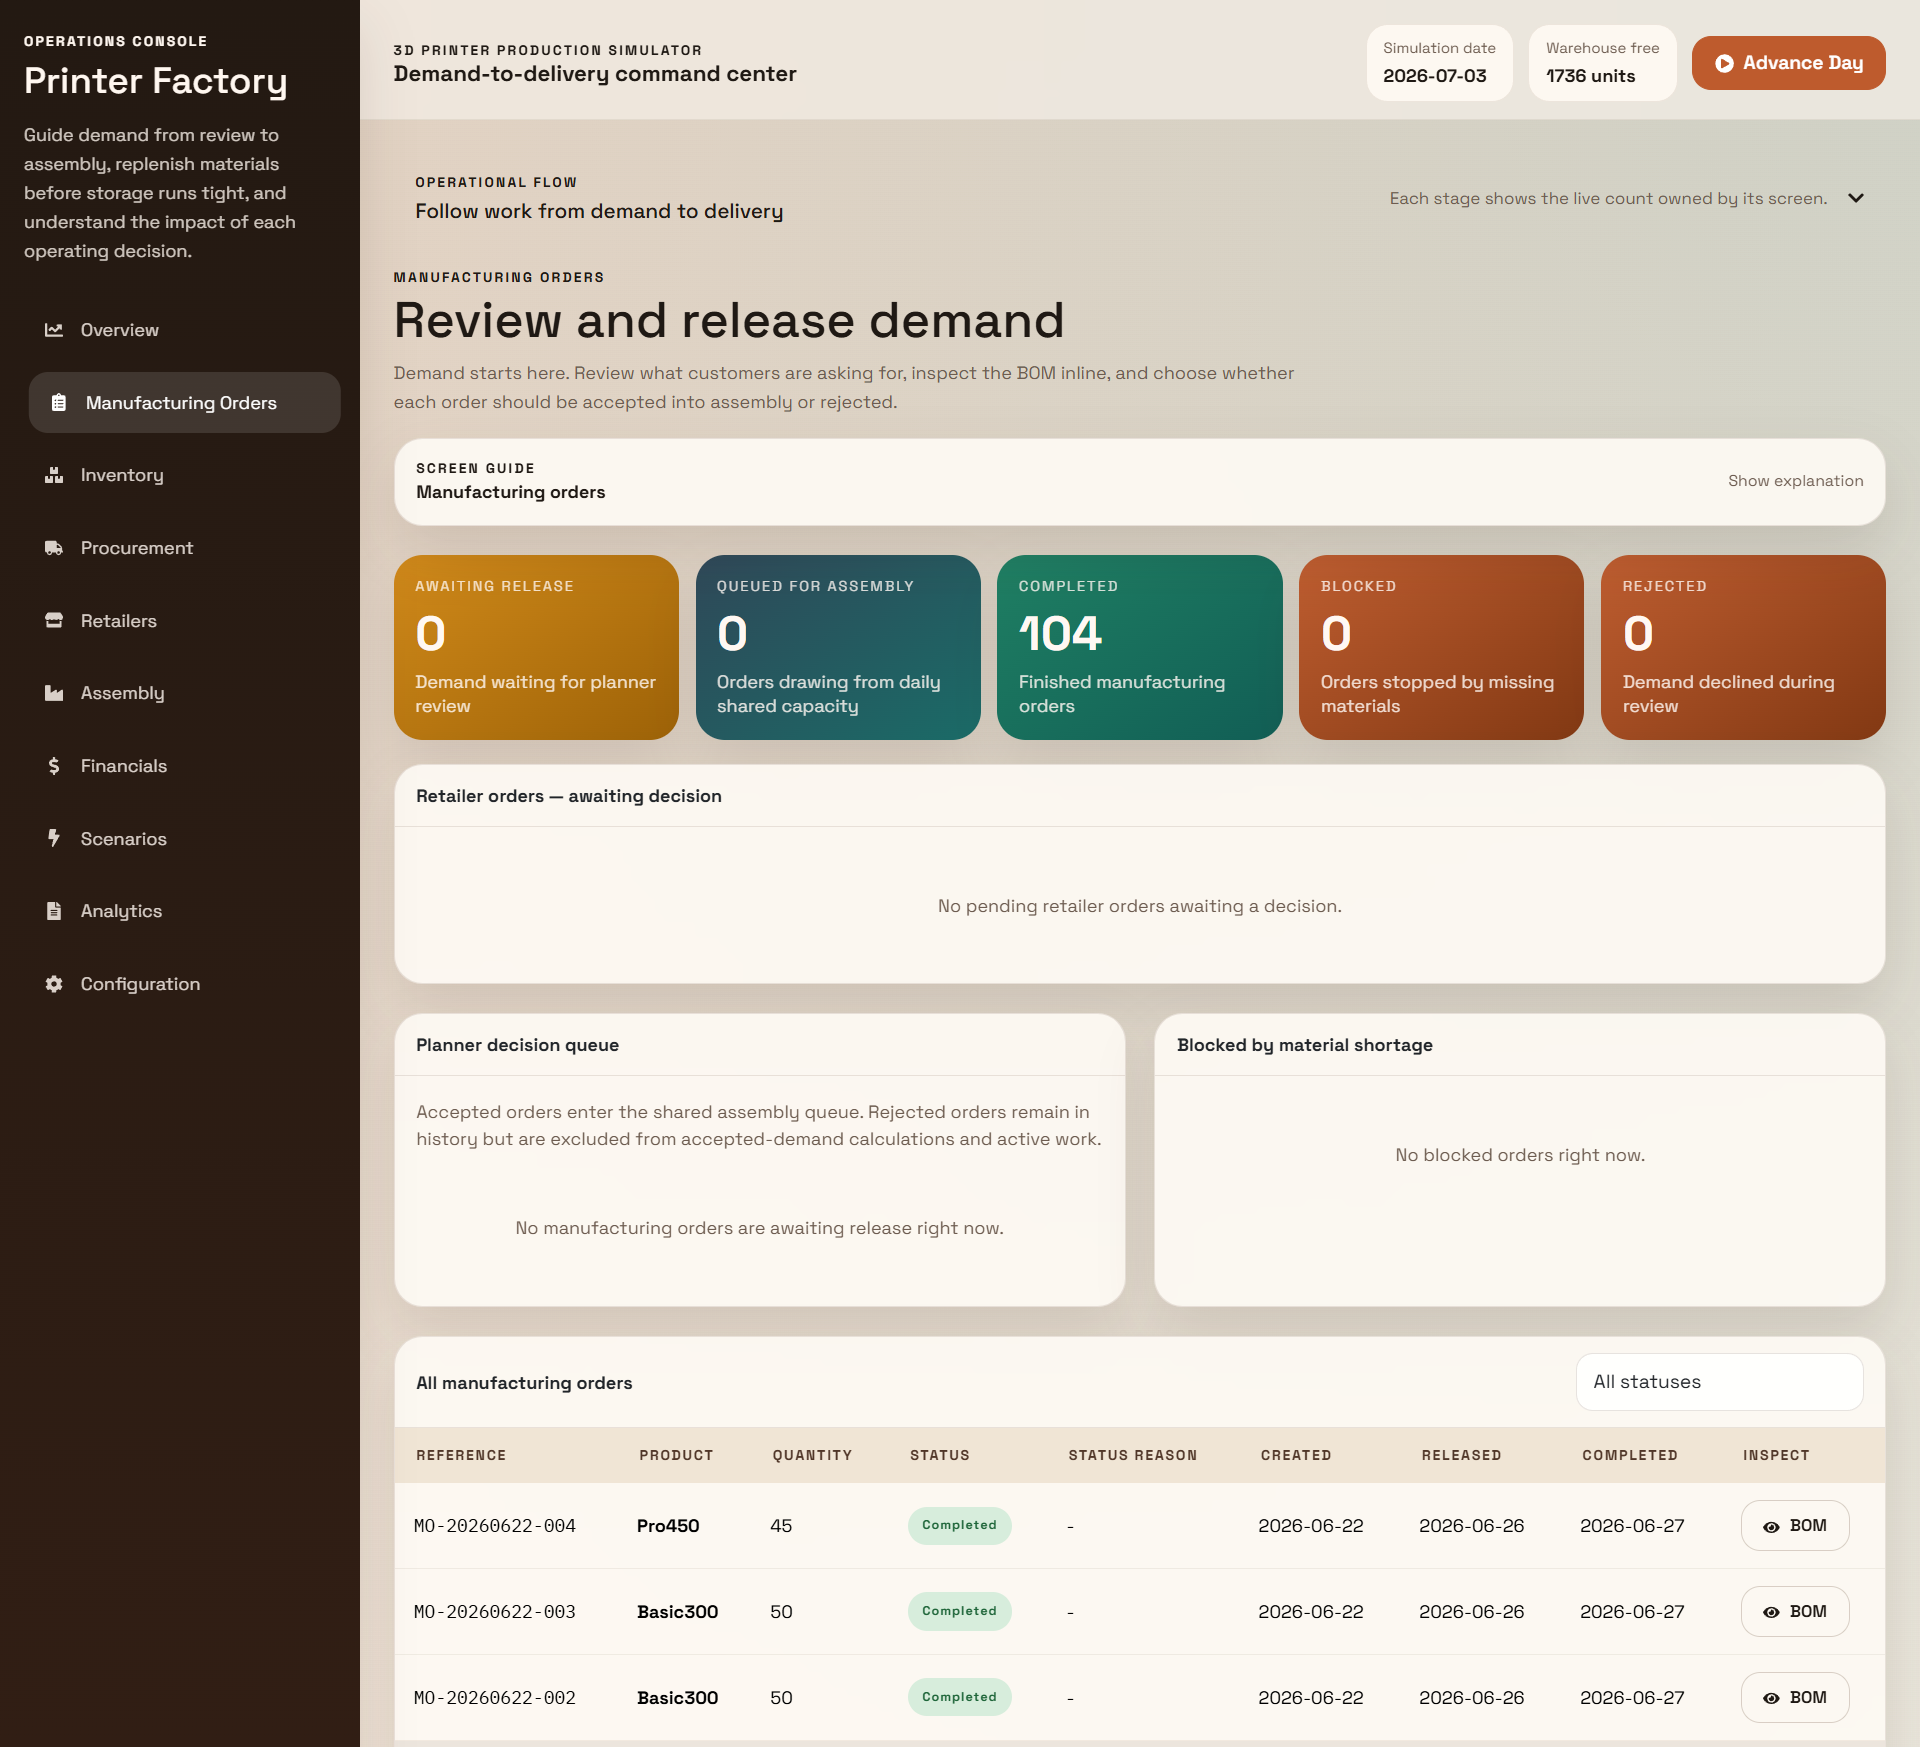
\includegraphics[width=0.55\textwidth]{images/capturas rush/orders-HR.png}
\caption{Orders page}
\end{figure}

\begin{figure}[H]
\centering
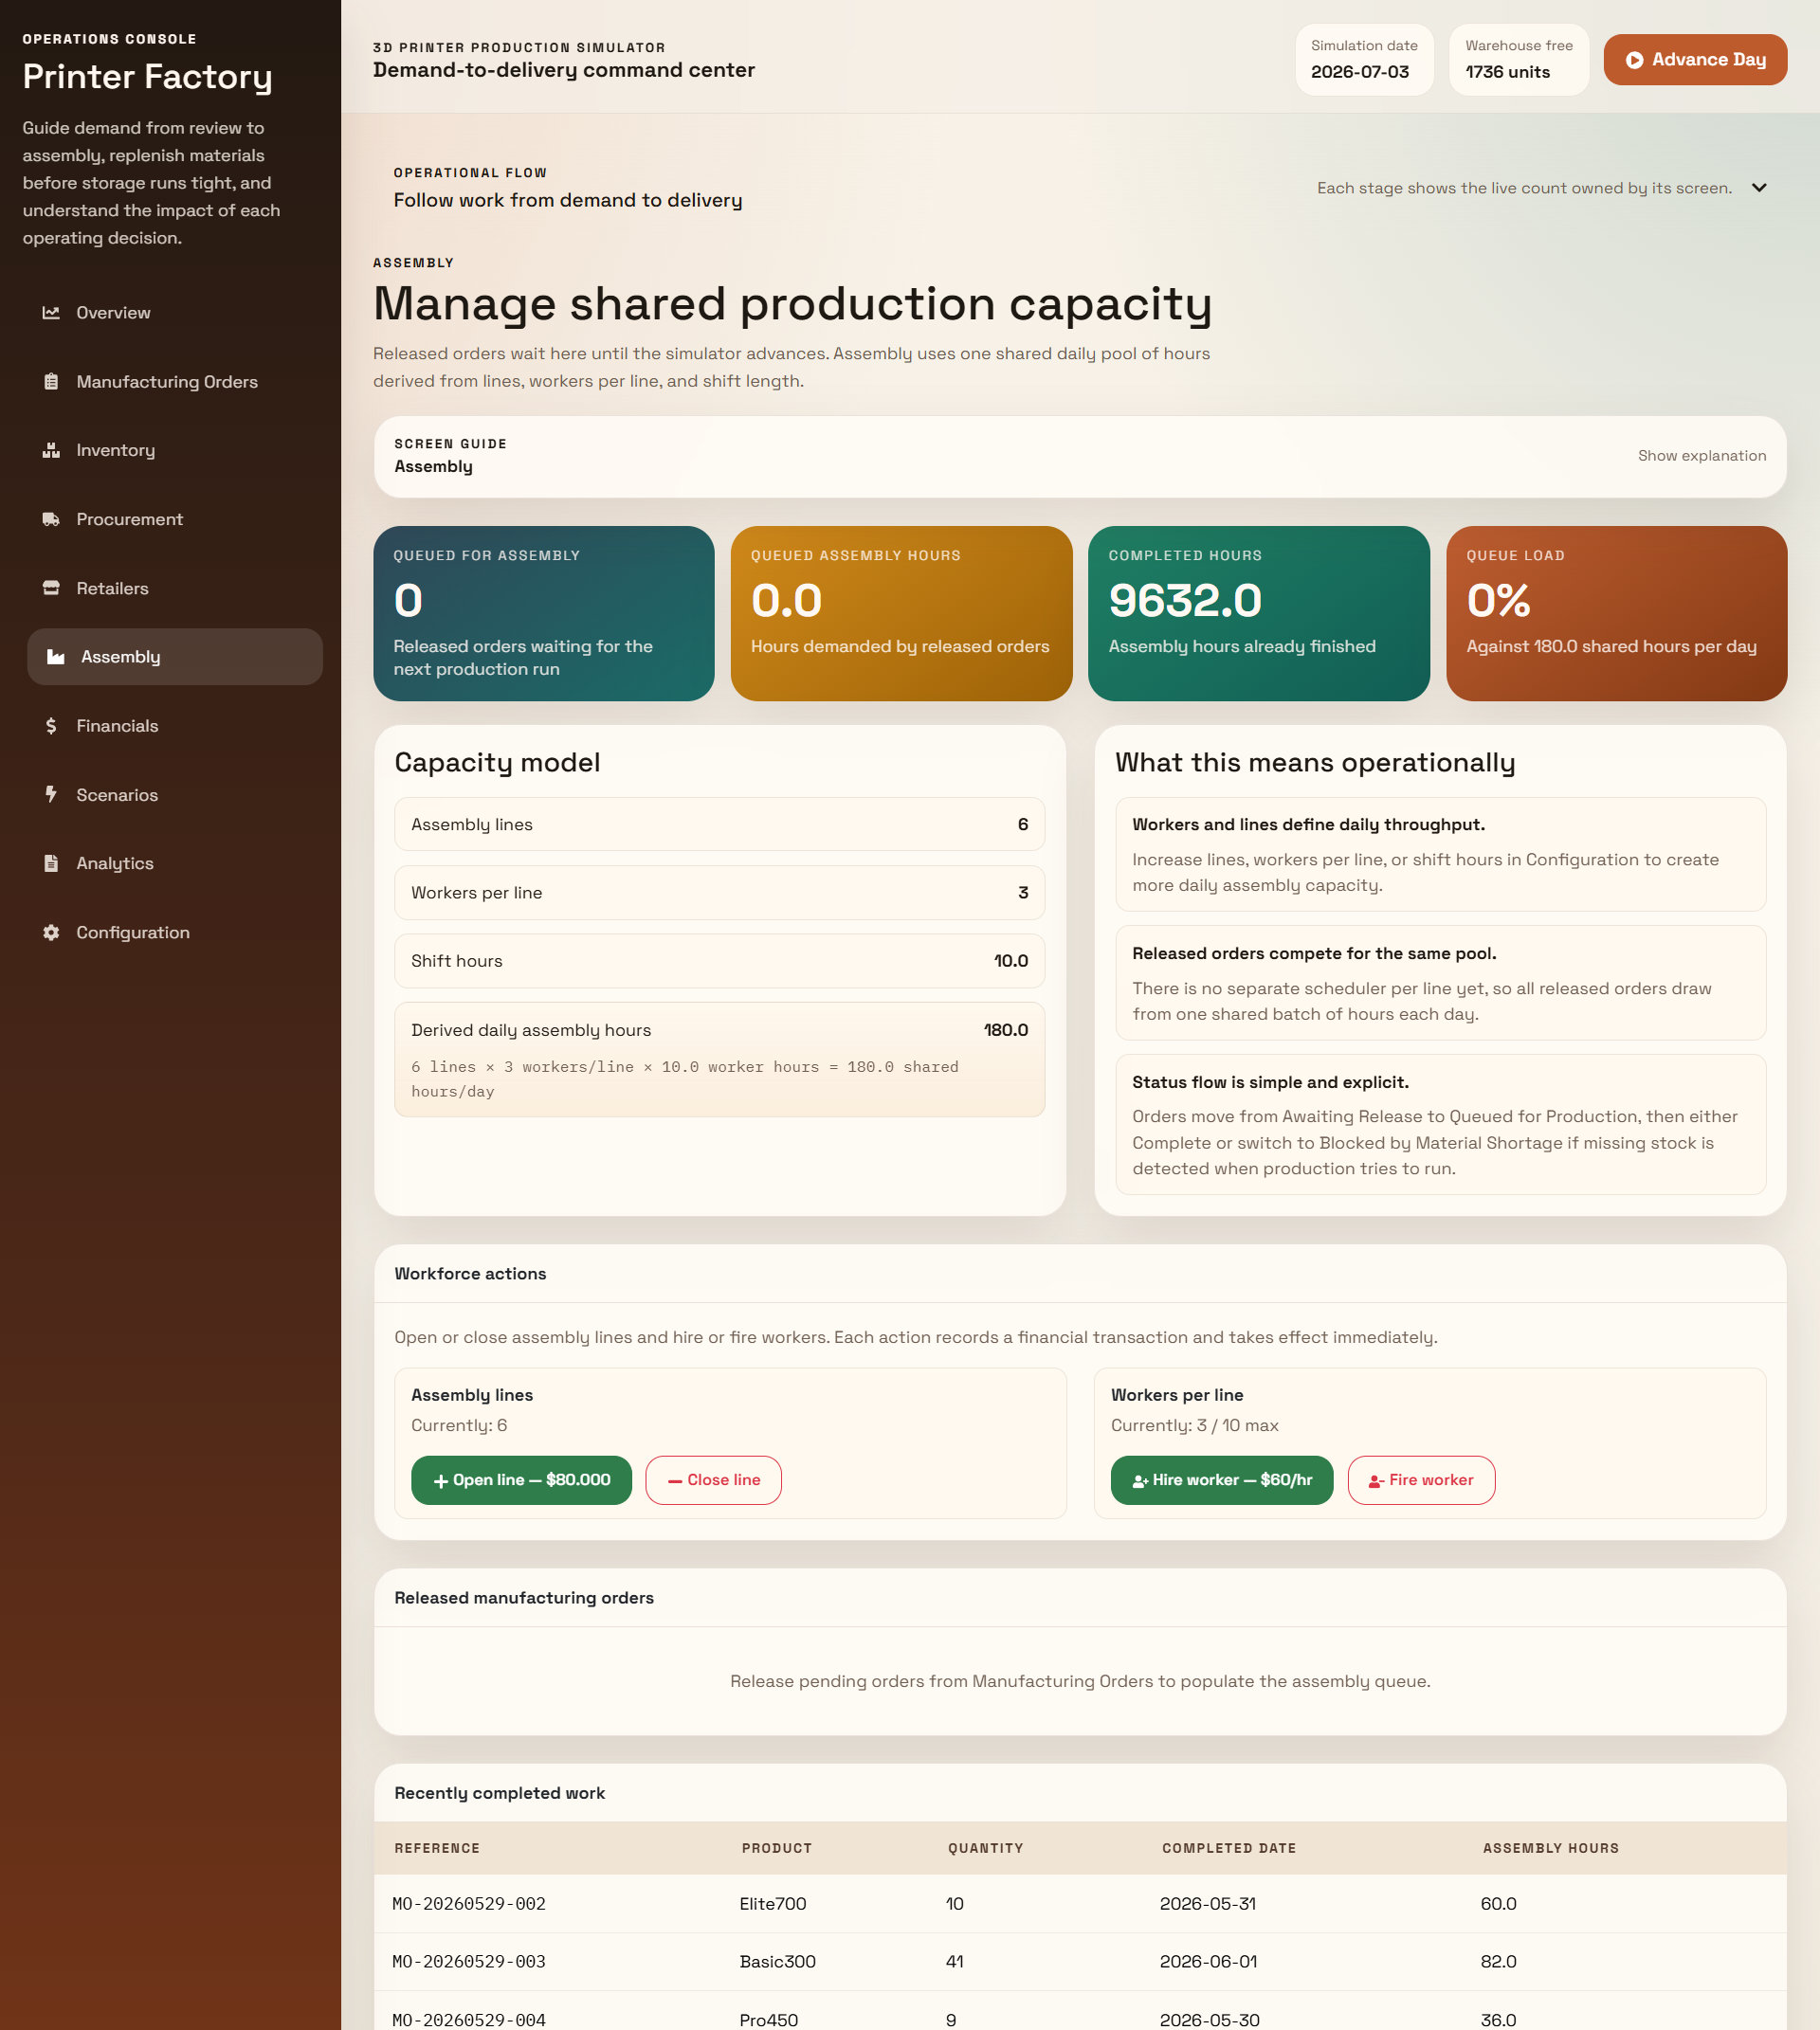
\includegraphics[width=0.55\textwidth]{images/capturas rush/production-HR.png}
\caption{Production page}
\end{figure}

\item \textbf{Production}: shows the assembly queue: active manufacturing
orders, queued assembly hours, daily capacity, and the number of workers
and lines.

\begin{figure}[H]
\centering
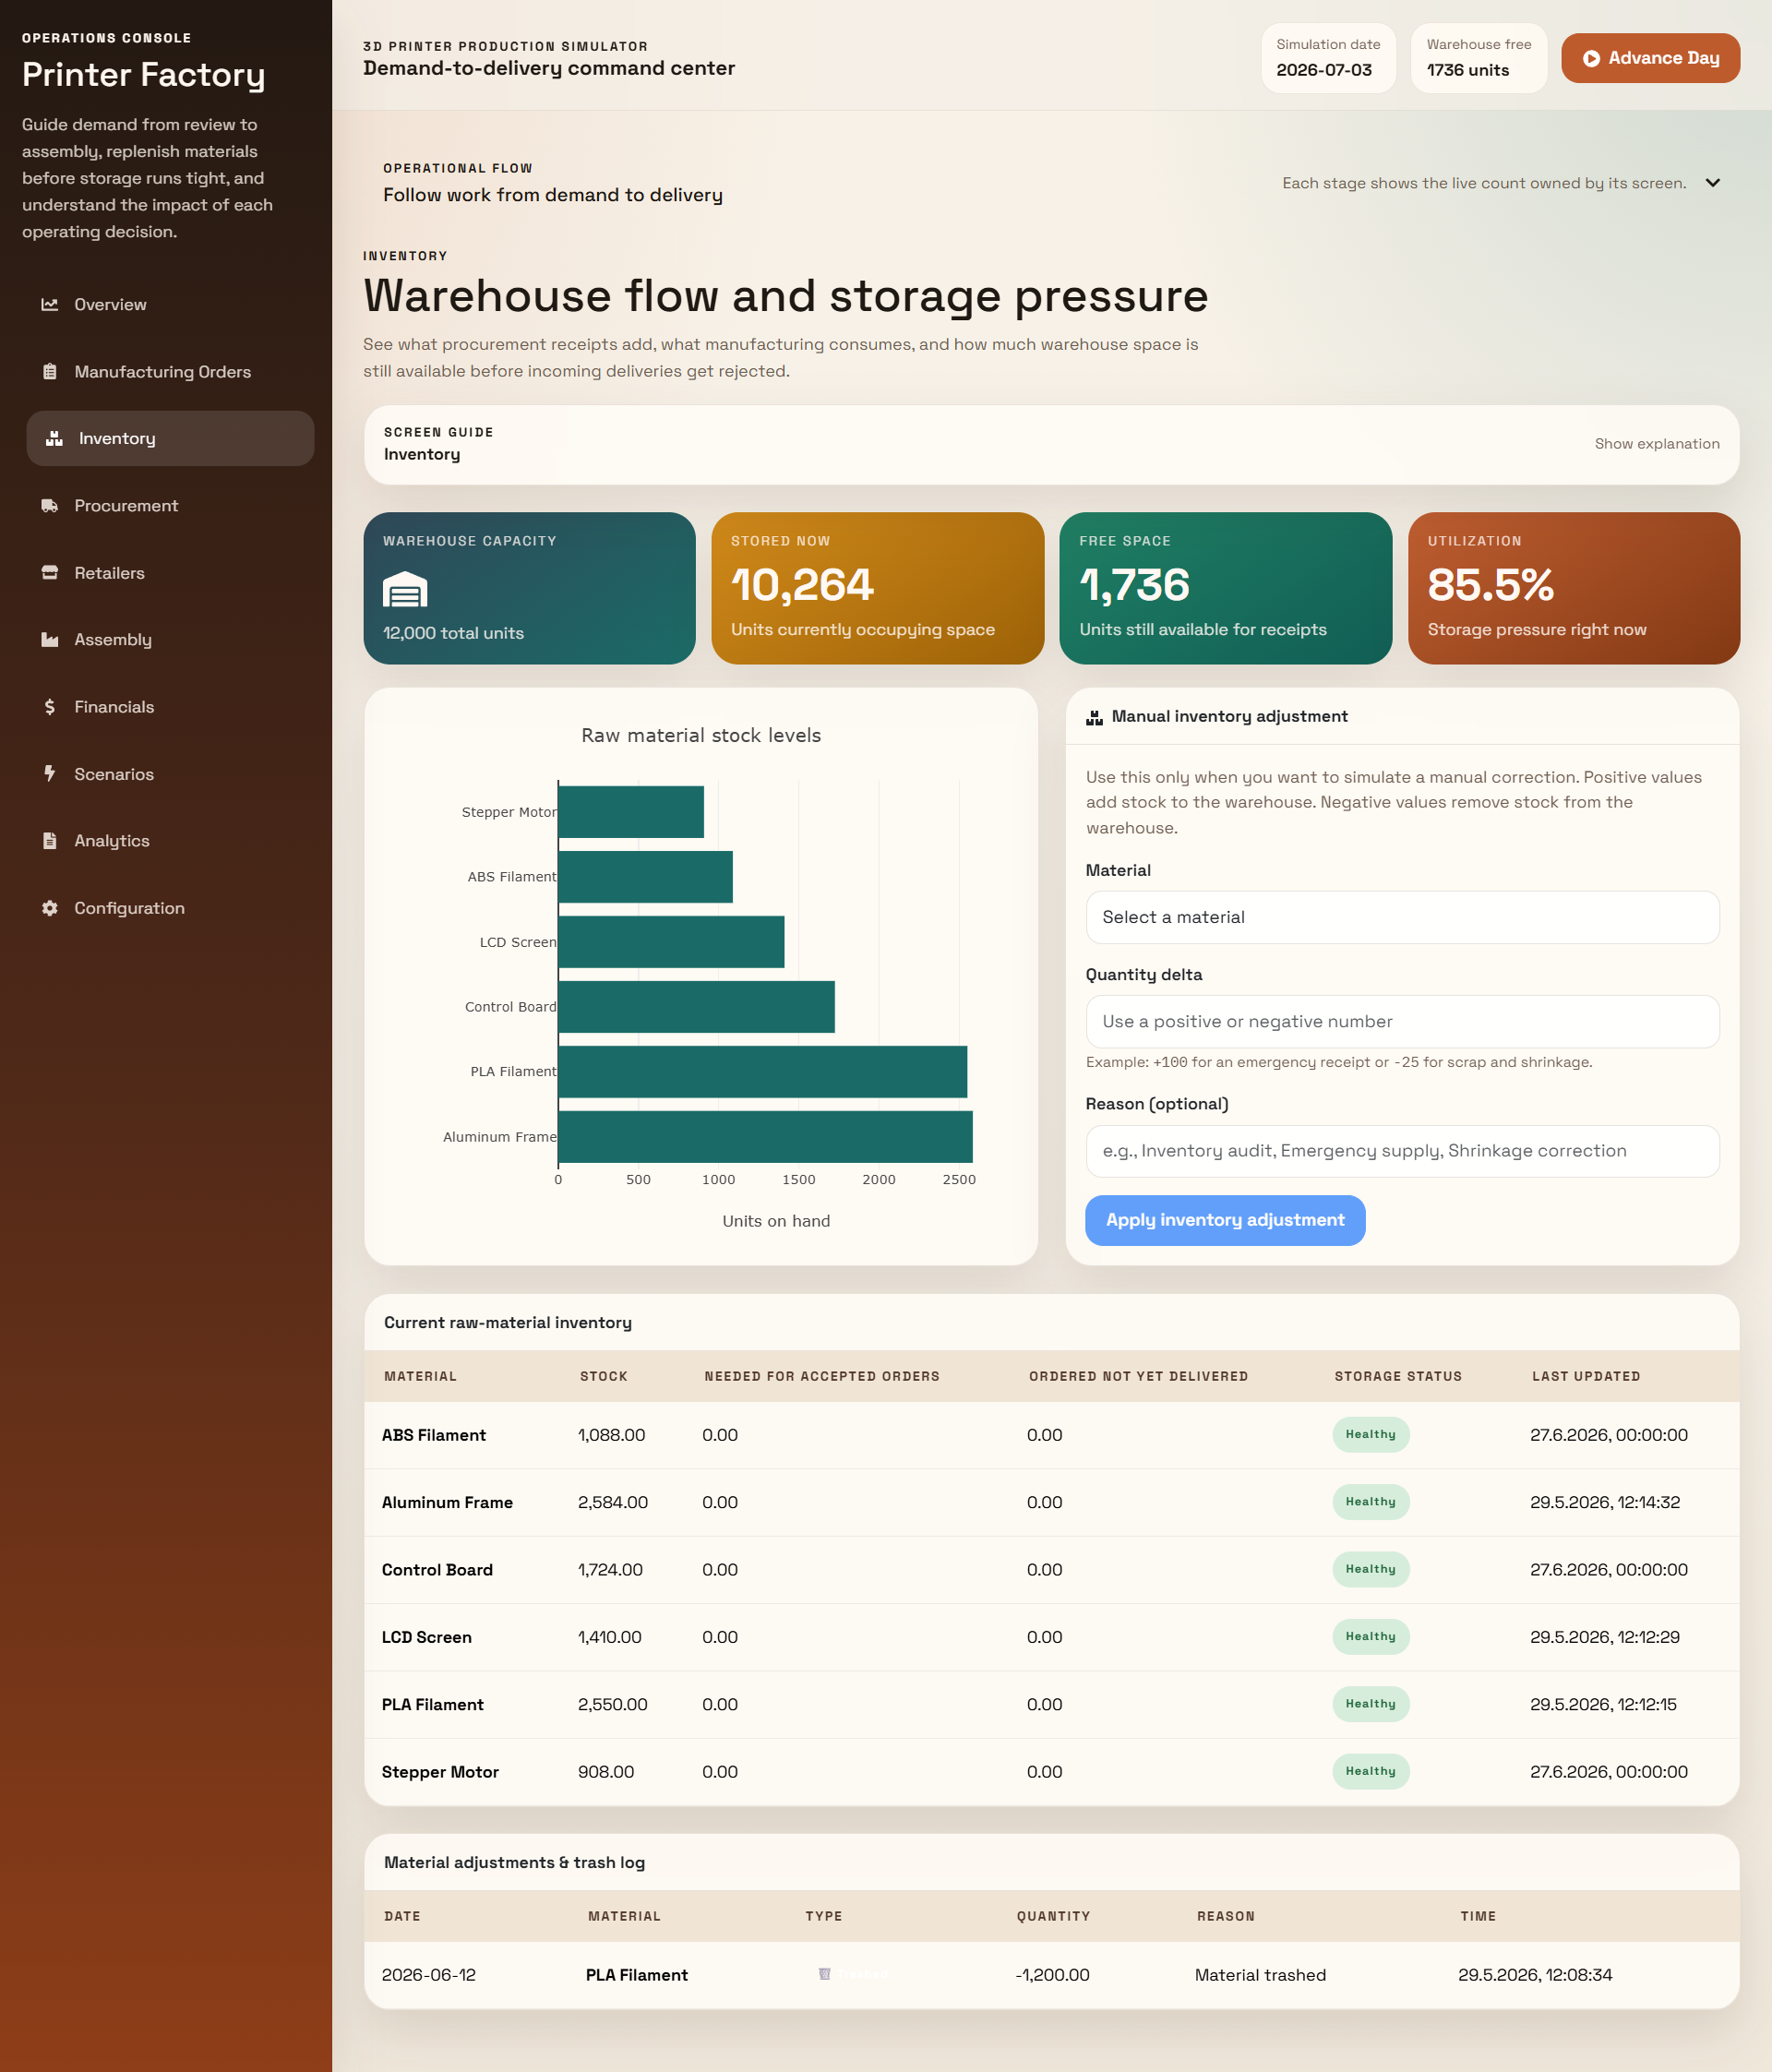
\includegraphics[width=0.45\textwidth]{images/capturas rush/inventory-HR.png}
\caption{Inventory page}
\end{figure}

\item \textbf{Inventory}: displays current stock for all six raw materials alongside their floor targets and the ``trashable'' surplus. Colour-coded status flags (CRITICAL, FLOOR, EXCESS) mirror the flags the agent reads from the CLI.

\begin{figure}[H]
\centering
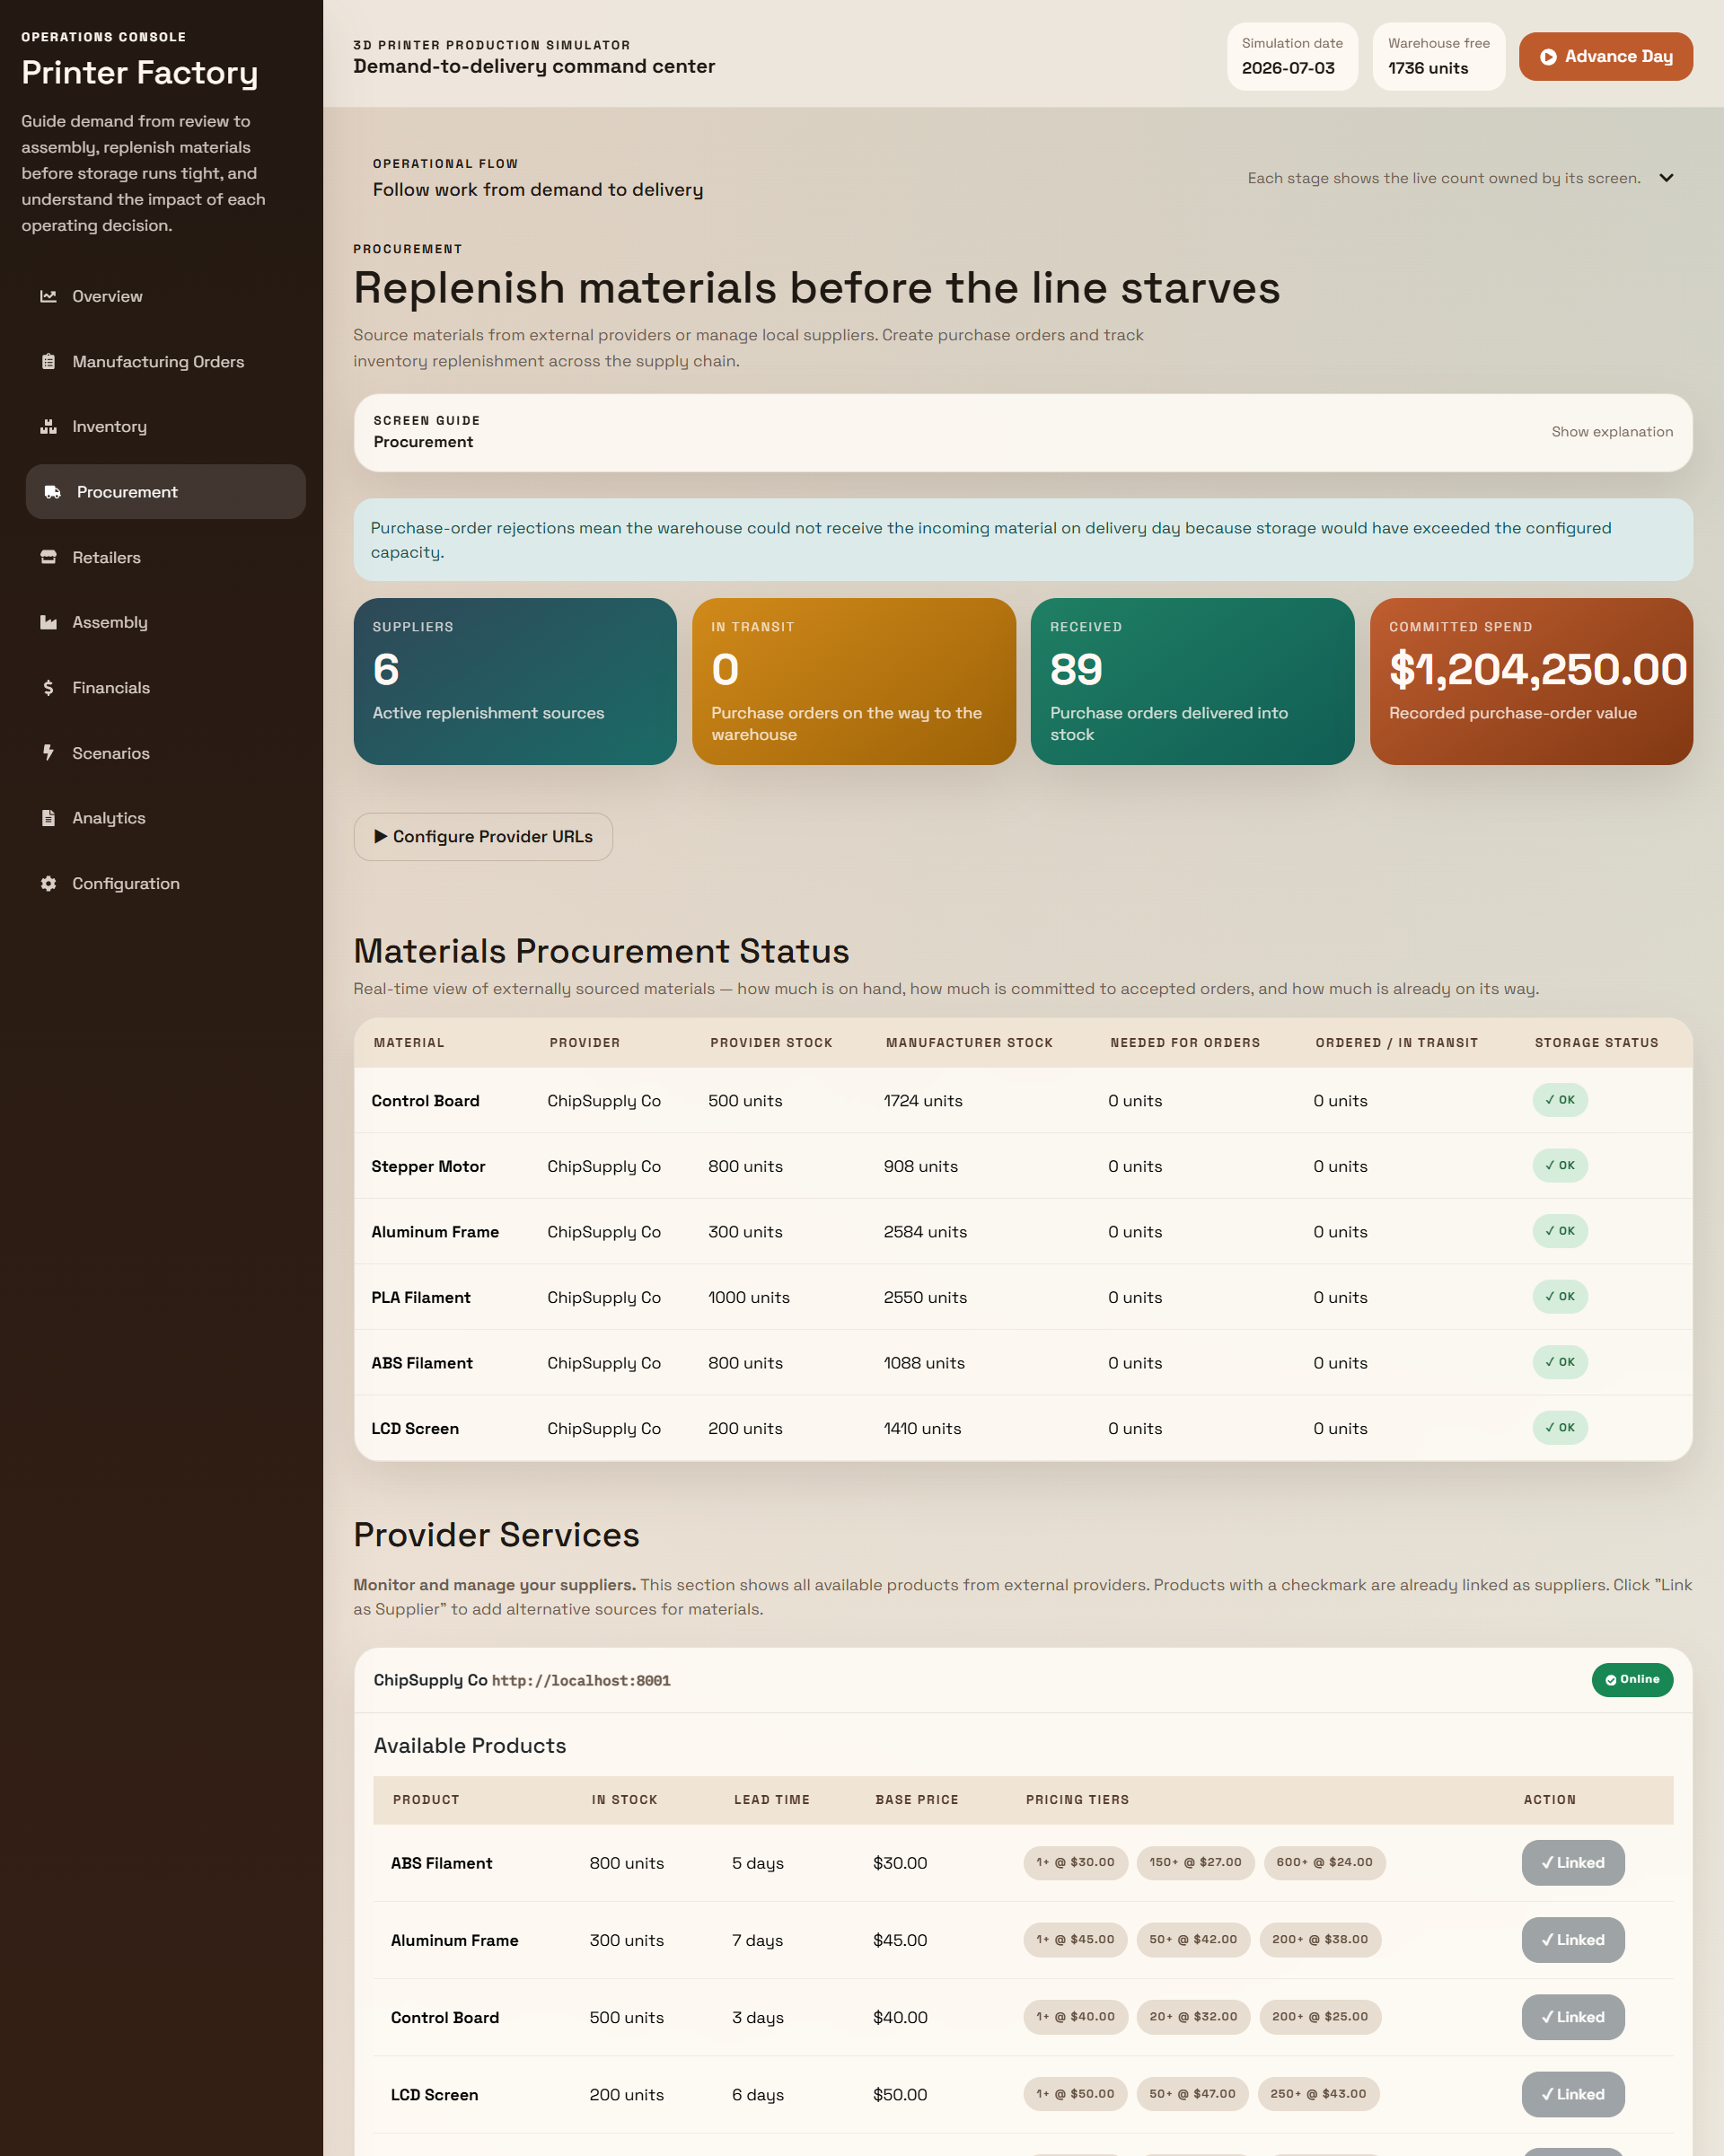
\includegraphics[width=0.45\textwidth]{images/capturas rush/suppliers-HR.png}
\caption{Suppliers page}
\end{figure}

\item \textbf{Suppliers}: lists all six suppliers with their lead times and
external provider wiring. Shows pending purchase orders in transit and their delivery days.

\begin{figure}[H]
\centering
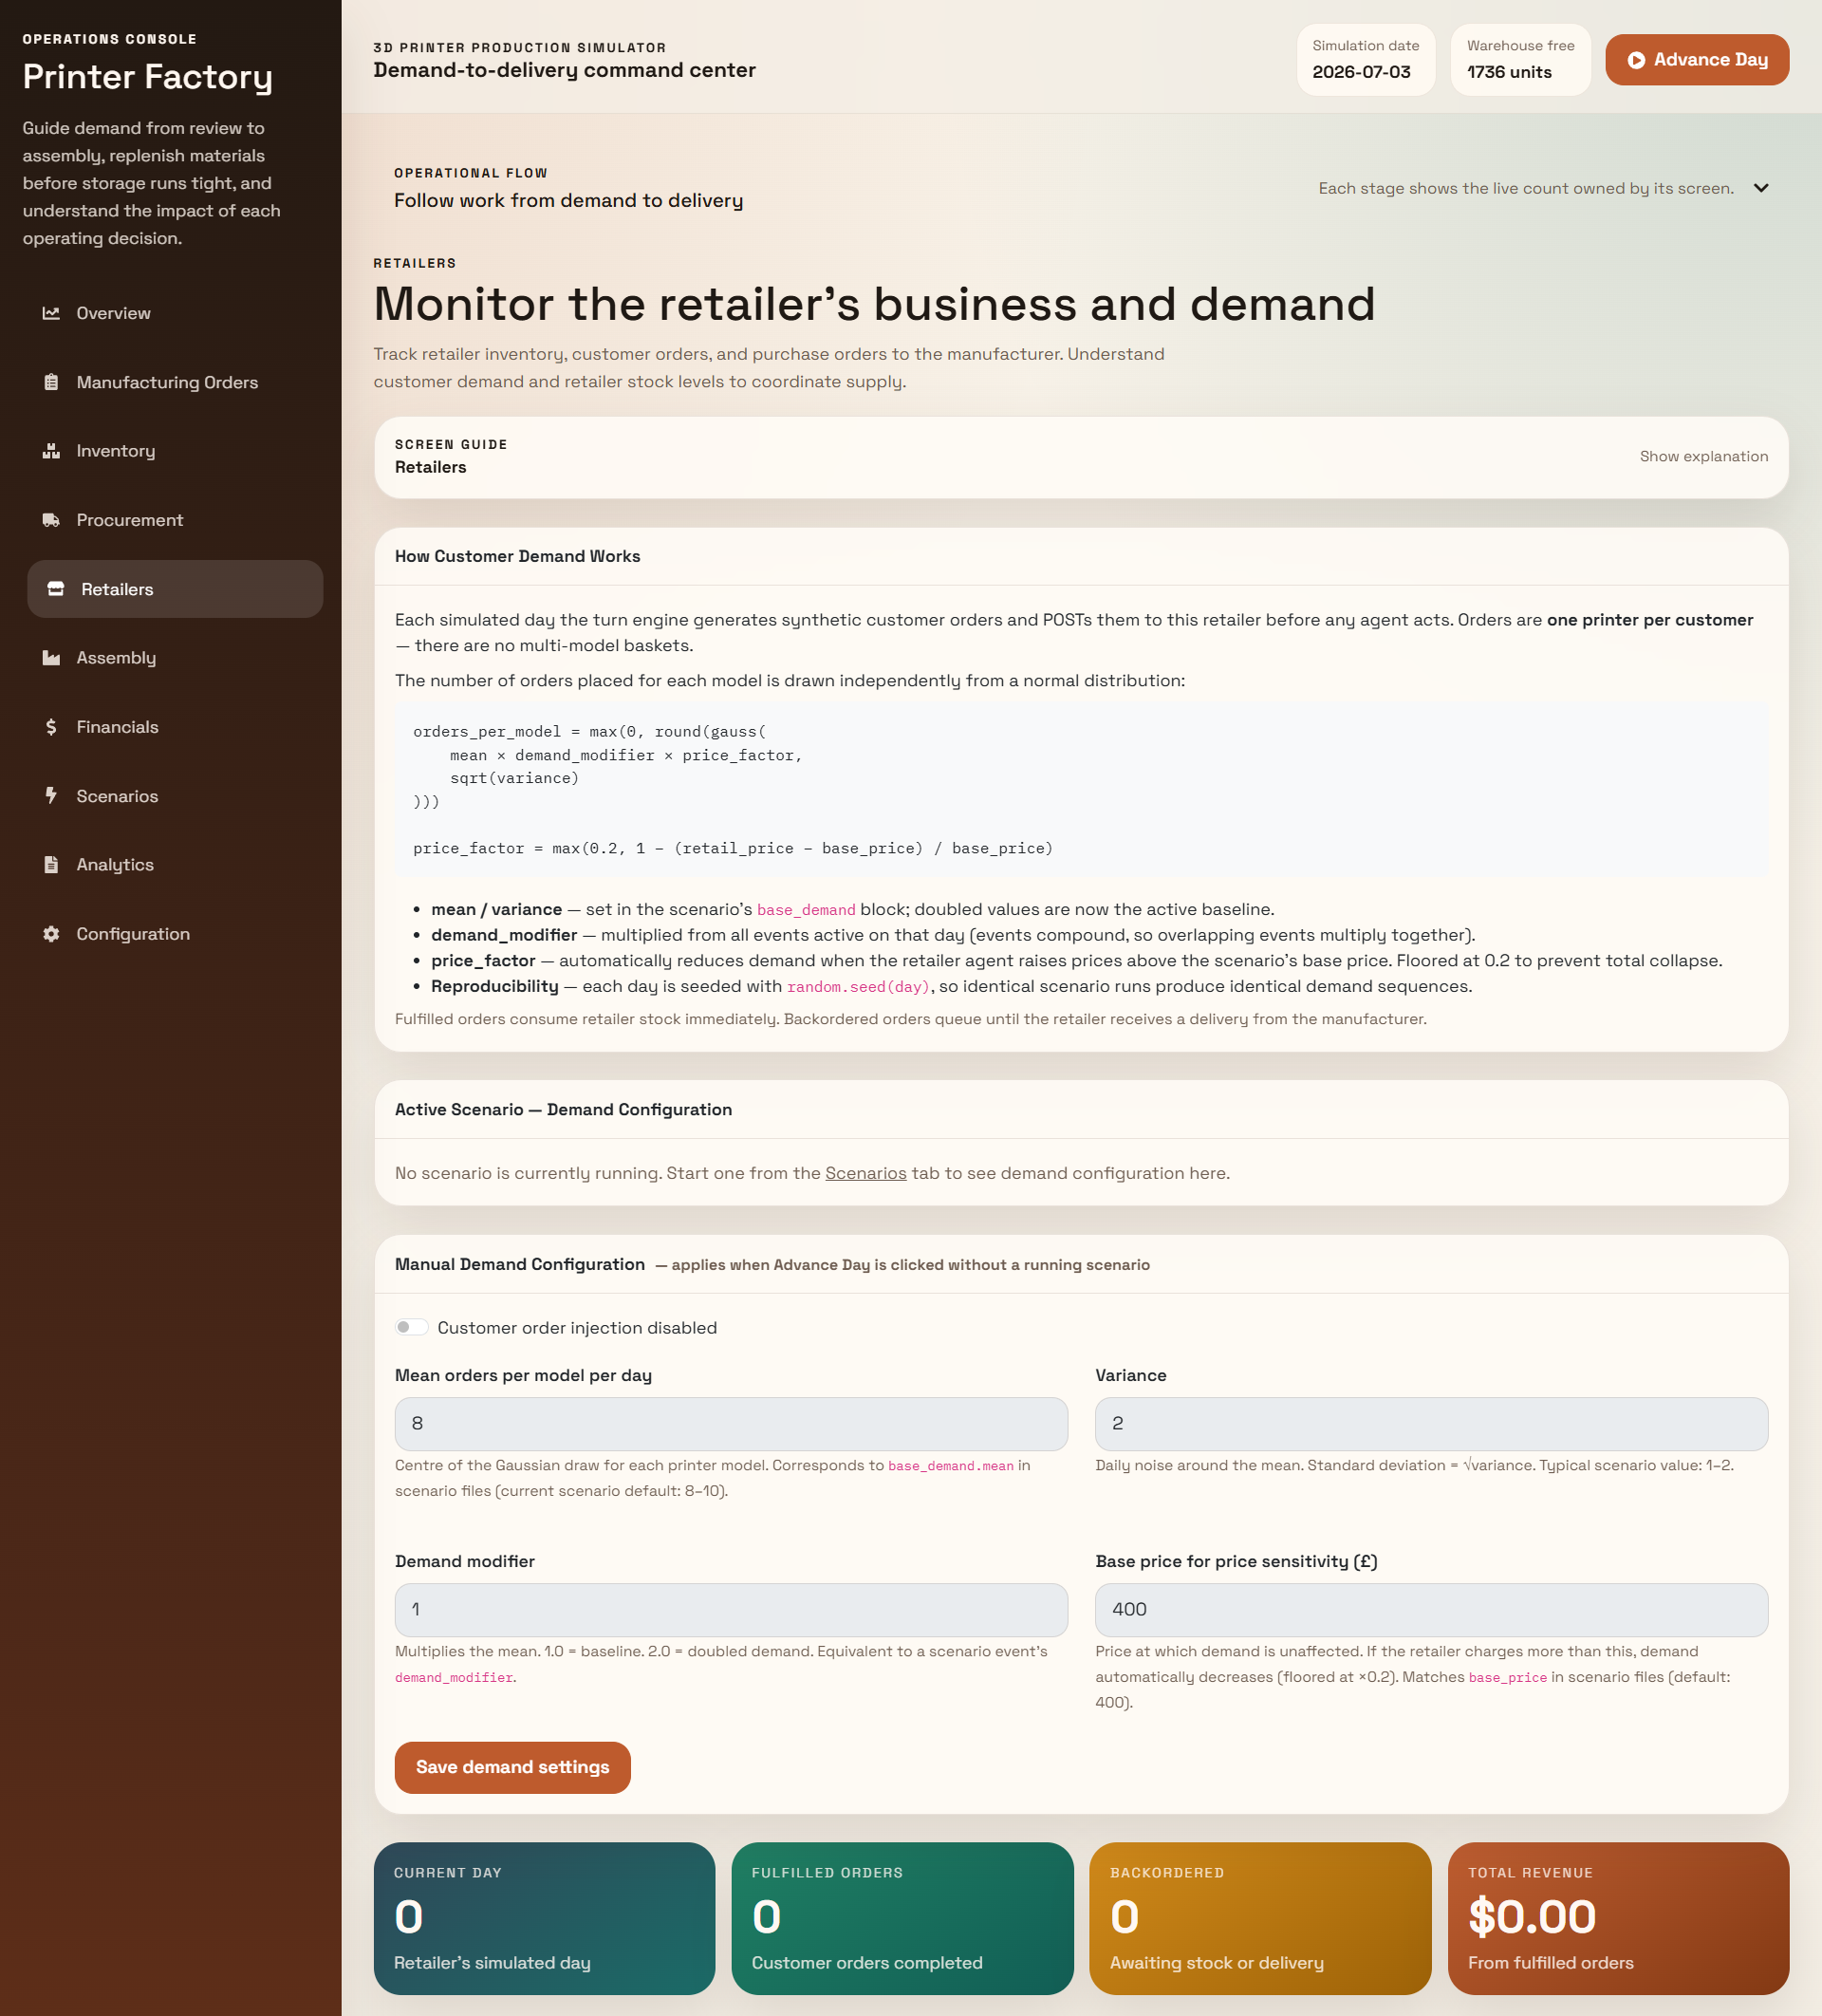
\includegraphics[width=0.5\textwidth]{images/capturas rush/retailers-HR.png}
\caption{Retailers page}
\end{figure}

\item \textbf{Retailers}: shows the connected retailer (PrinterWorld), the
sales orders it has placed, and delivery status. This is the
manufacturer's view of its downstream customer.
\begin{figure}[H]
\centering
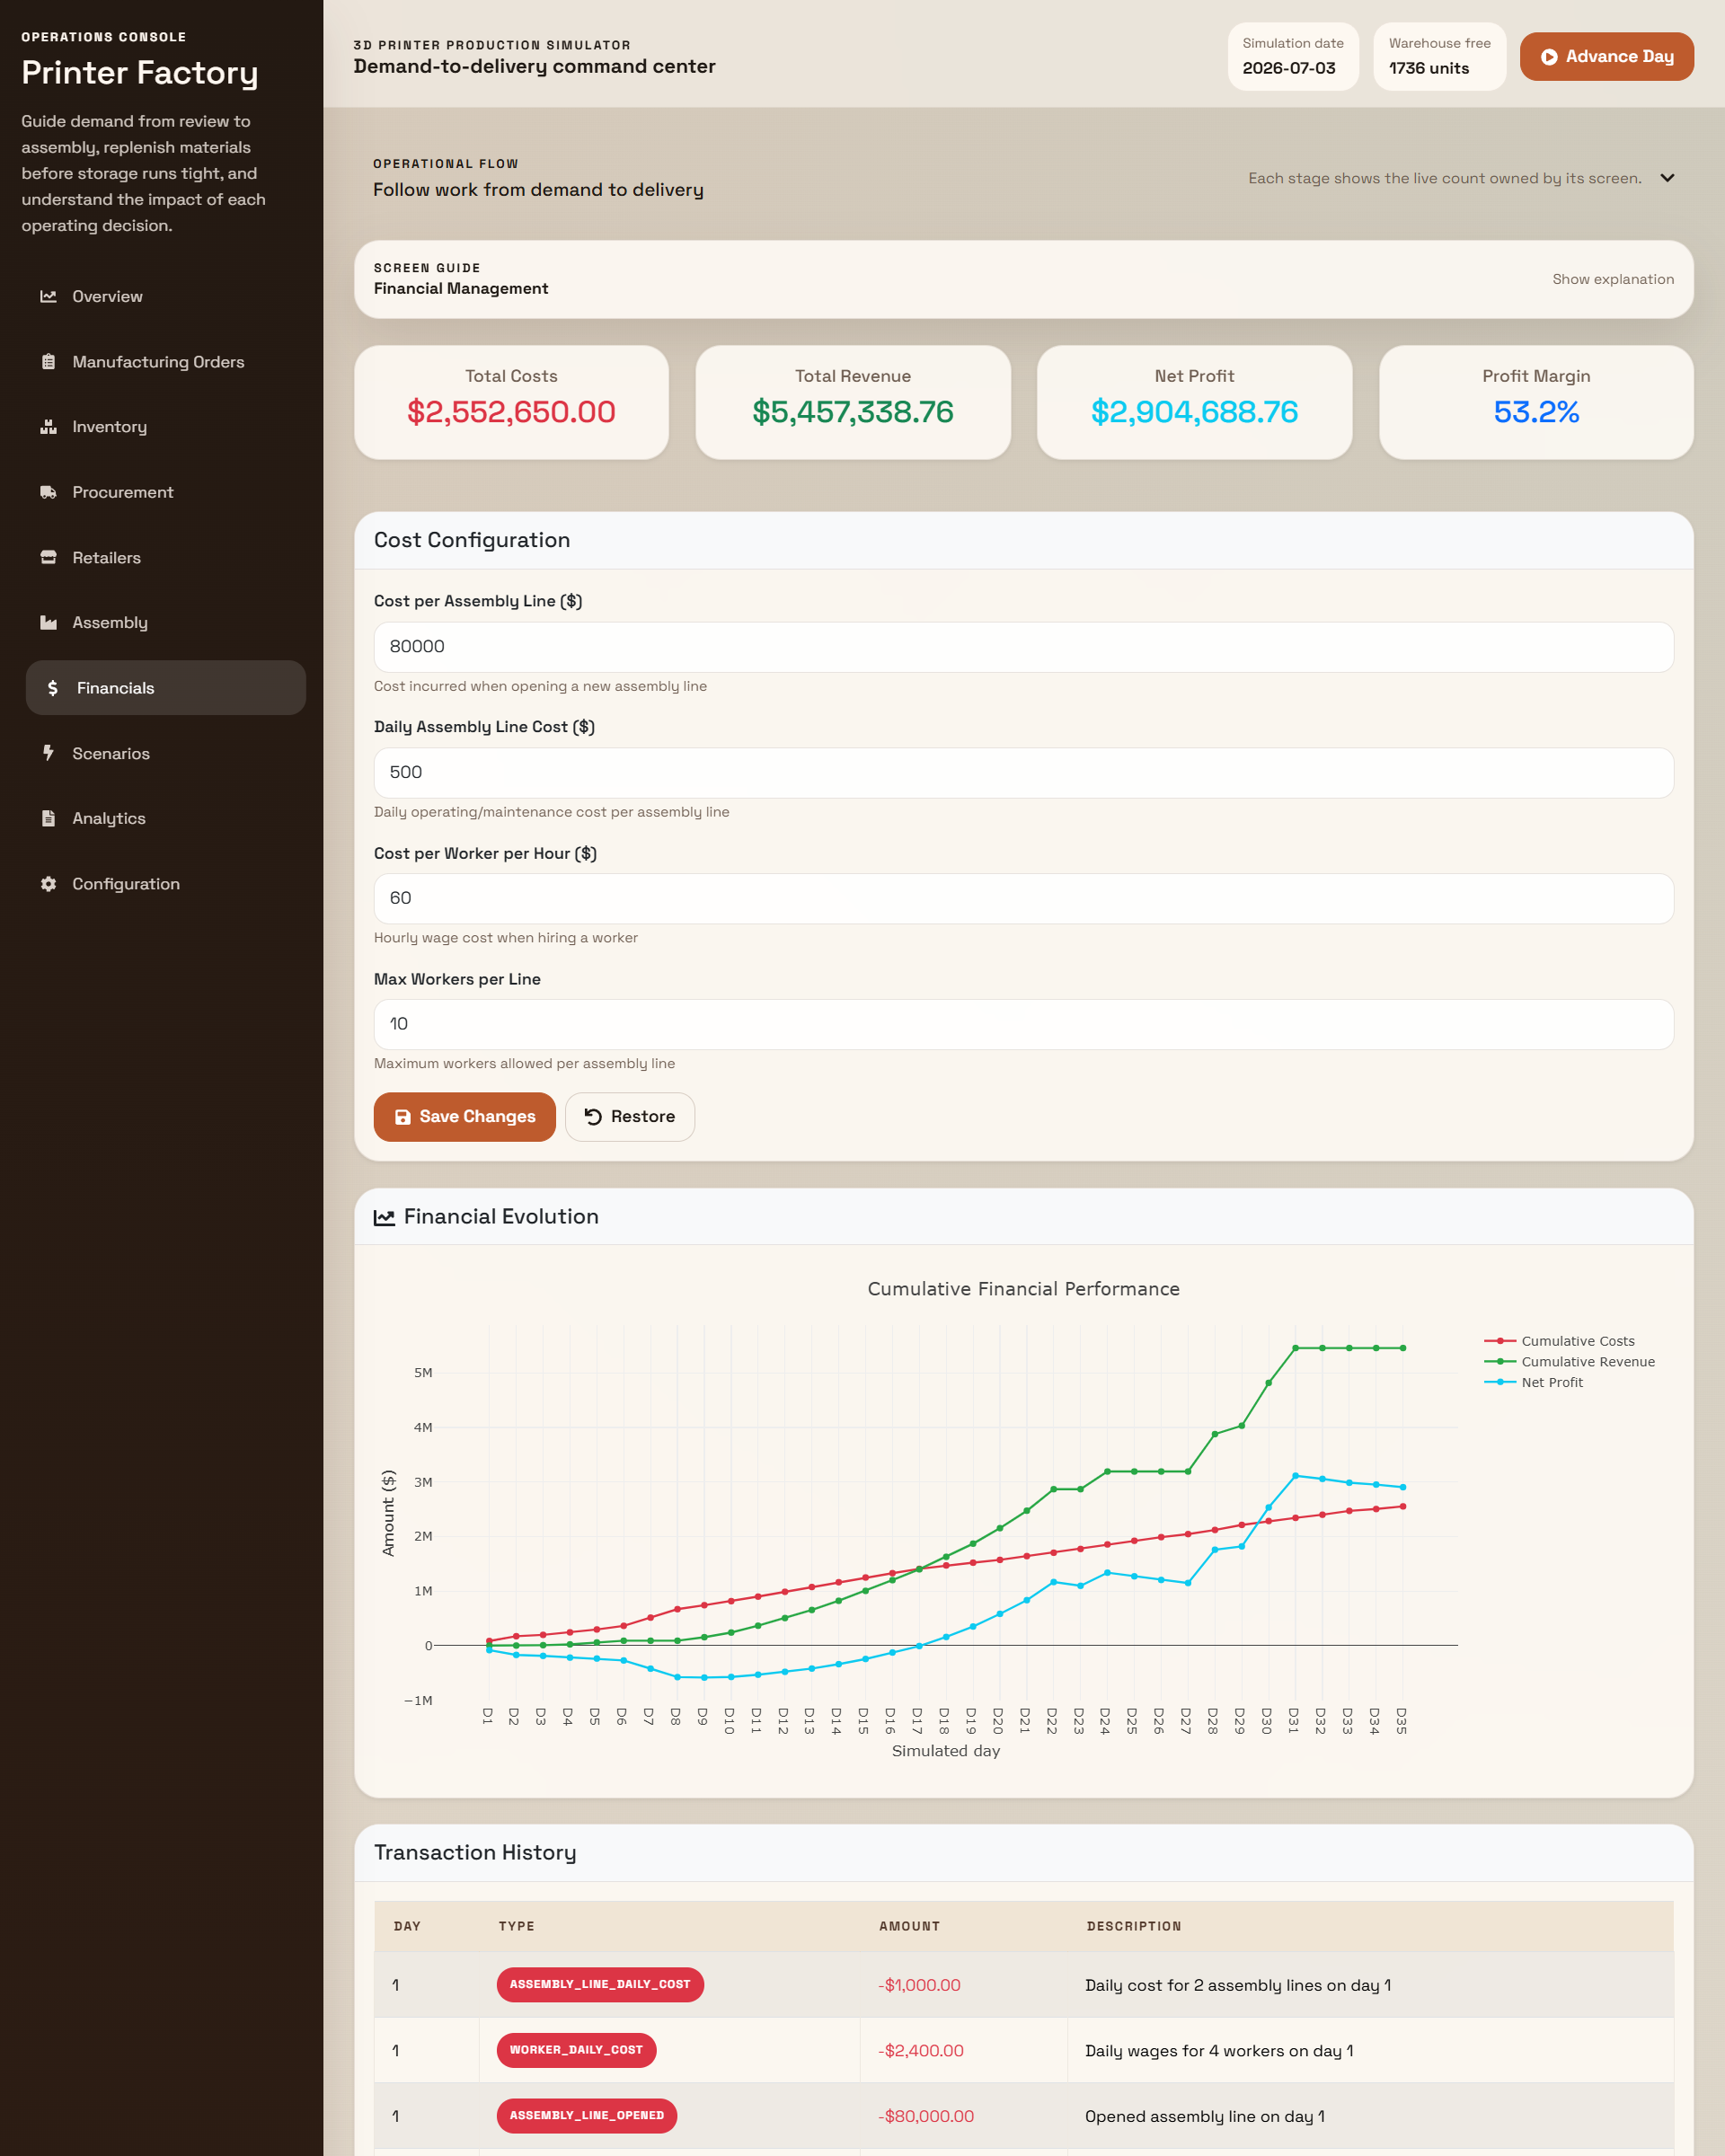
\includegraphics[width=0.45\textwidth]{images/capturas rush/financials-HR.png}
\caption{Financials page}
\end{figure}

\item \textbf{Financials}: running totals for revenue, material costs, labour
costs, and net profit. Updated each simulated day so the operator can
track whether the agent's pricing decisions are generating margin.

\begin{figure}[H]
\centering
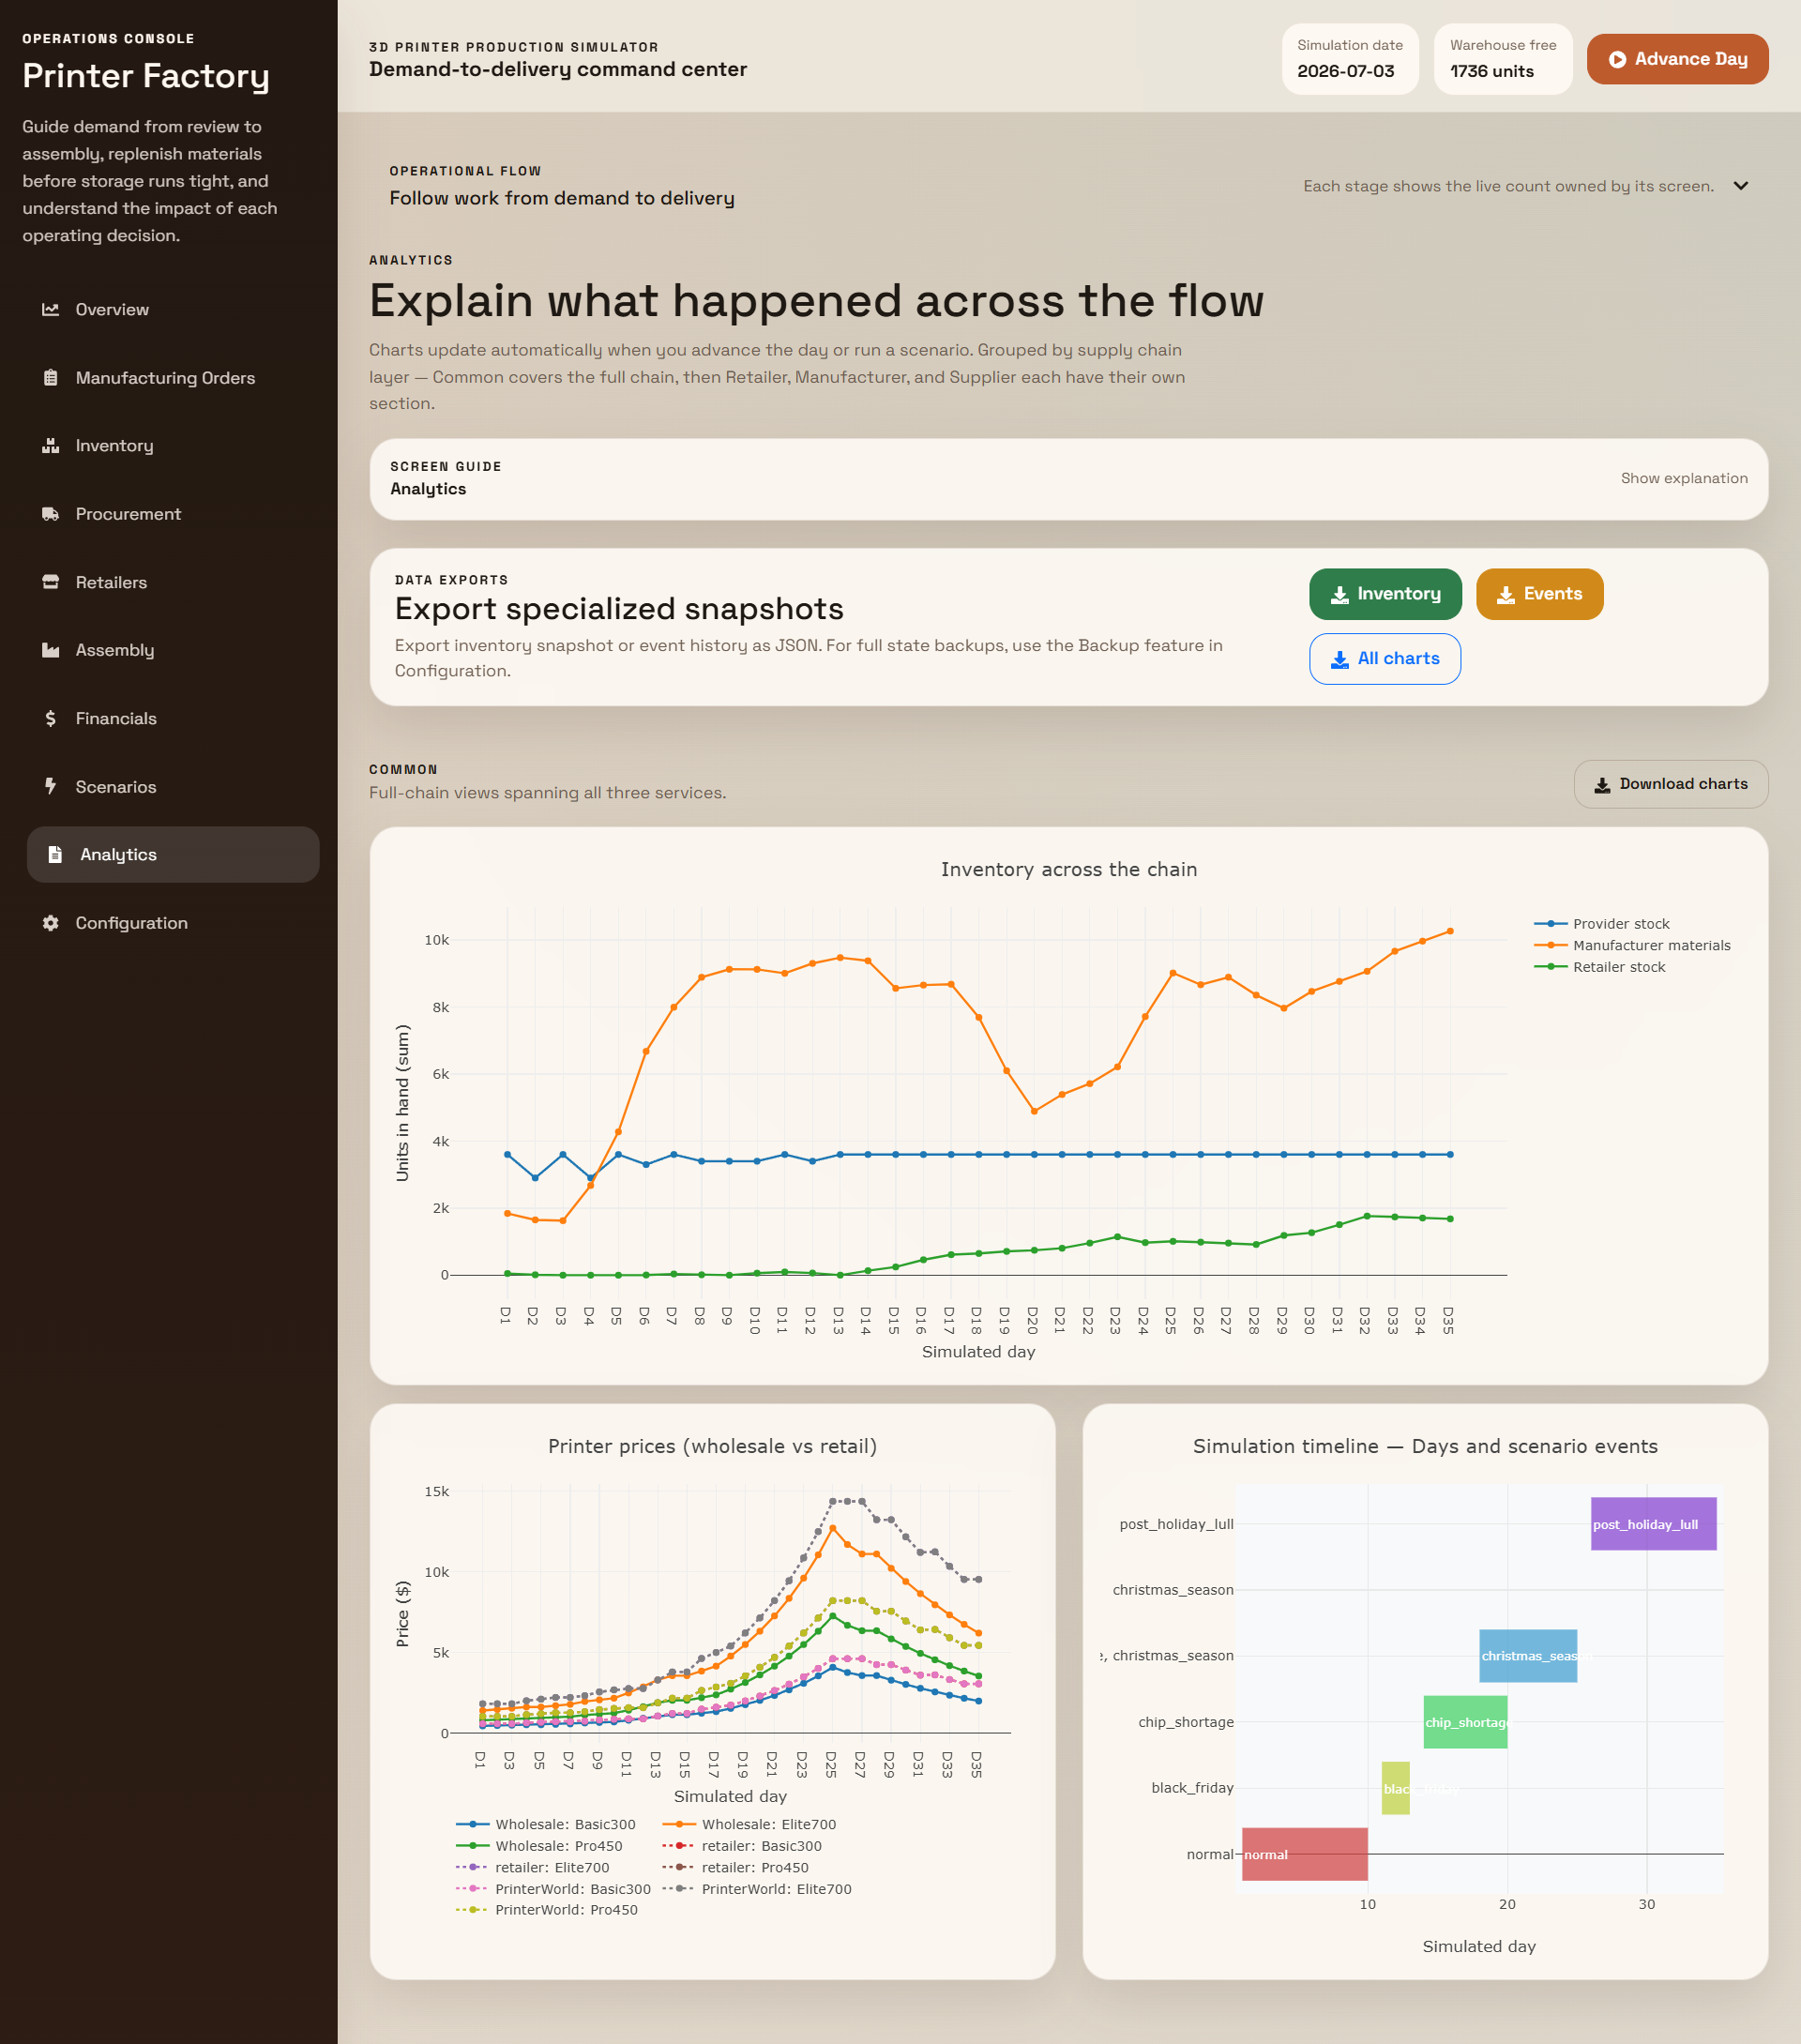
\includegraphics[width=0.45\textwidth]{images/capturas rush/reports-HR.png}
\caption{Reports page}
\end{figure}

\item \textbf{Reports}: per-day event log and summary statistics. The event
table is the audit trail: every state transition (order released,
delivery received, price changed) is recorded here.

\begin{figure}[H]
\centering
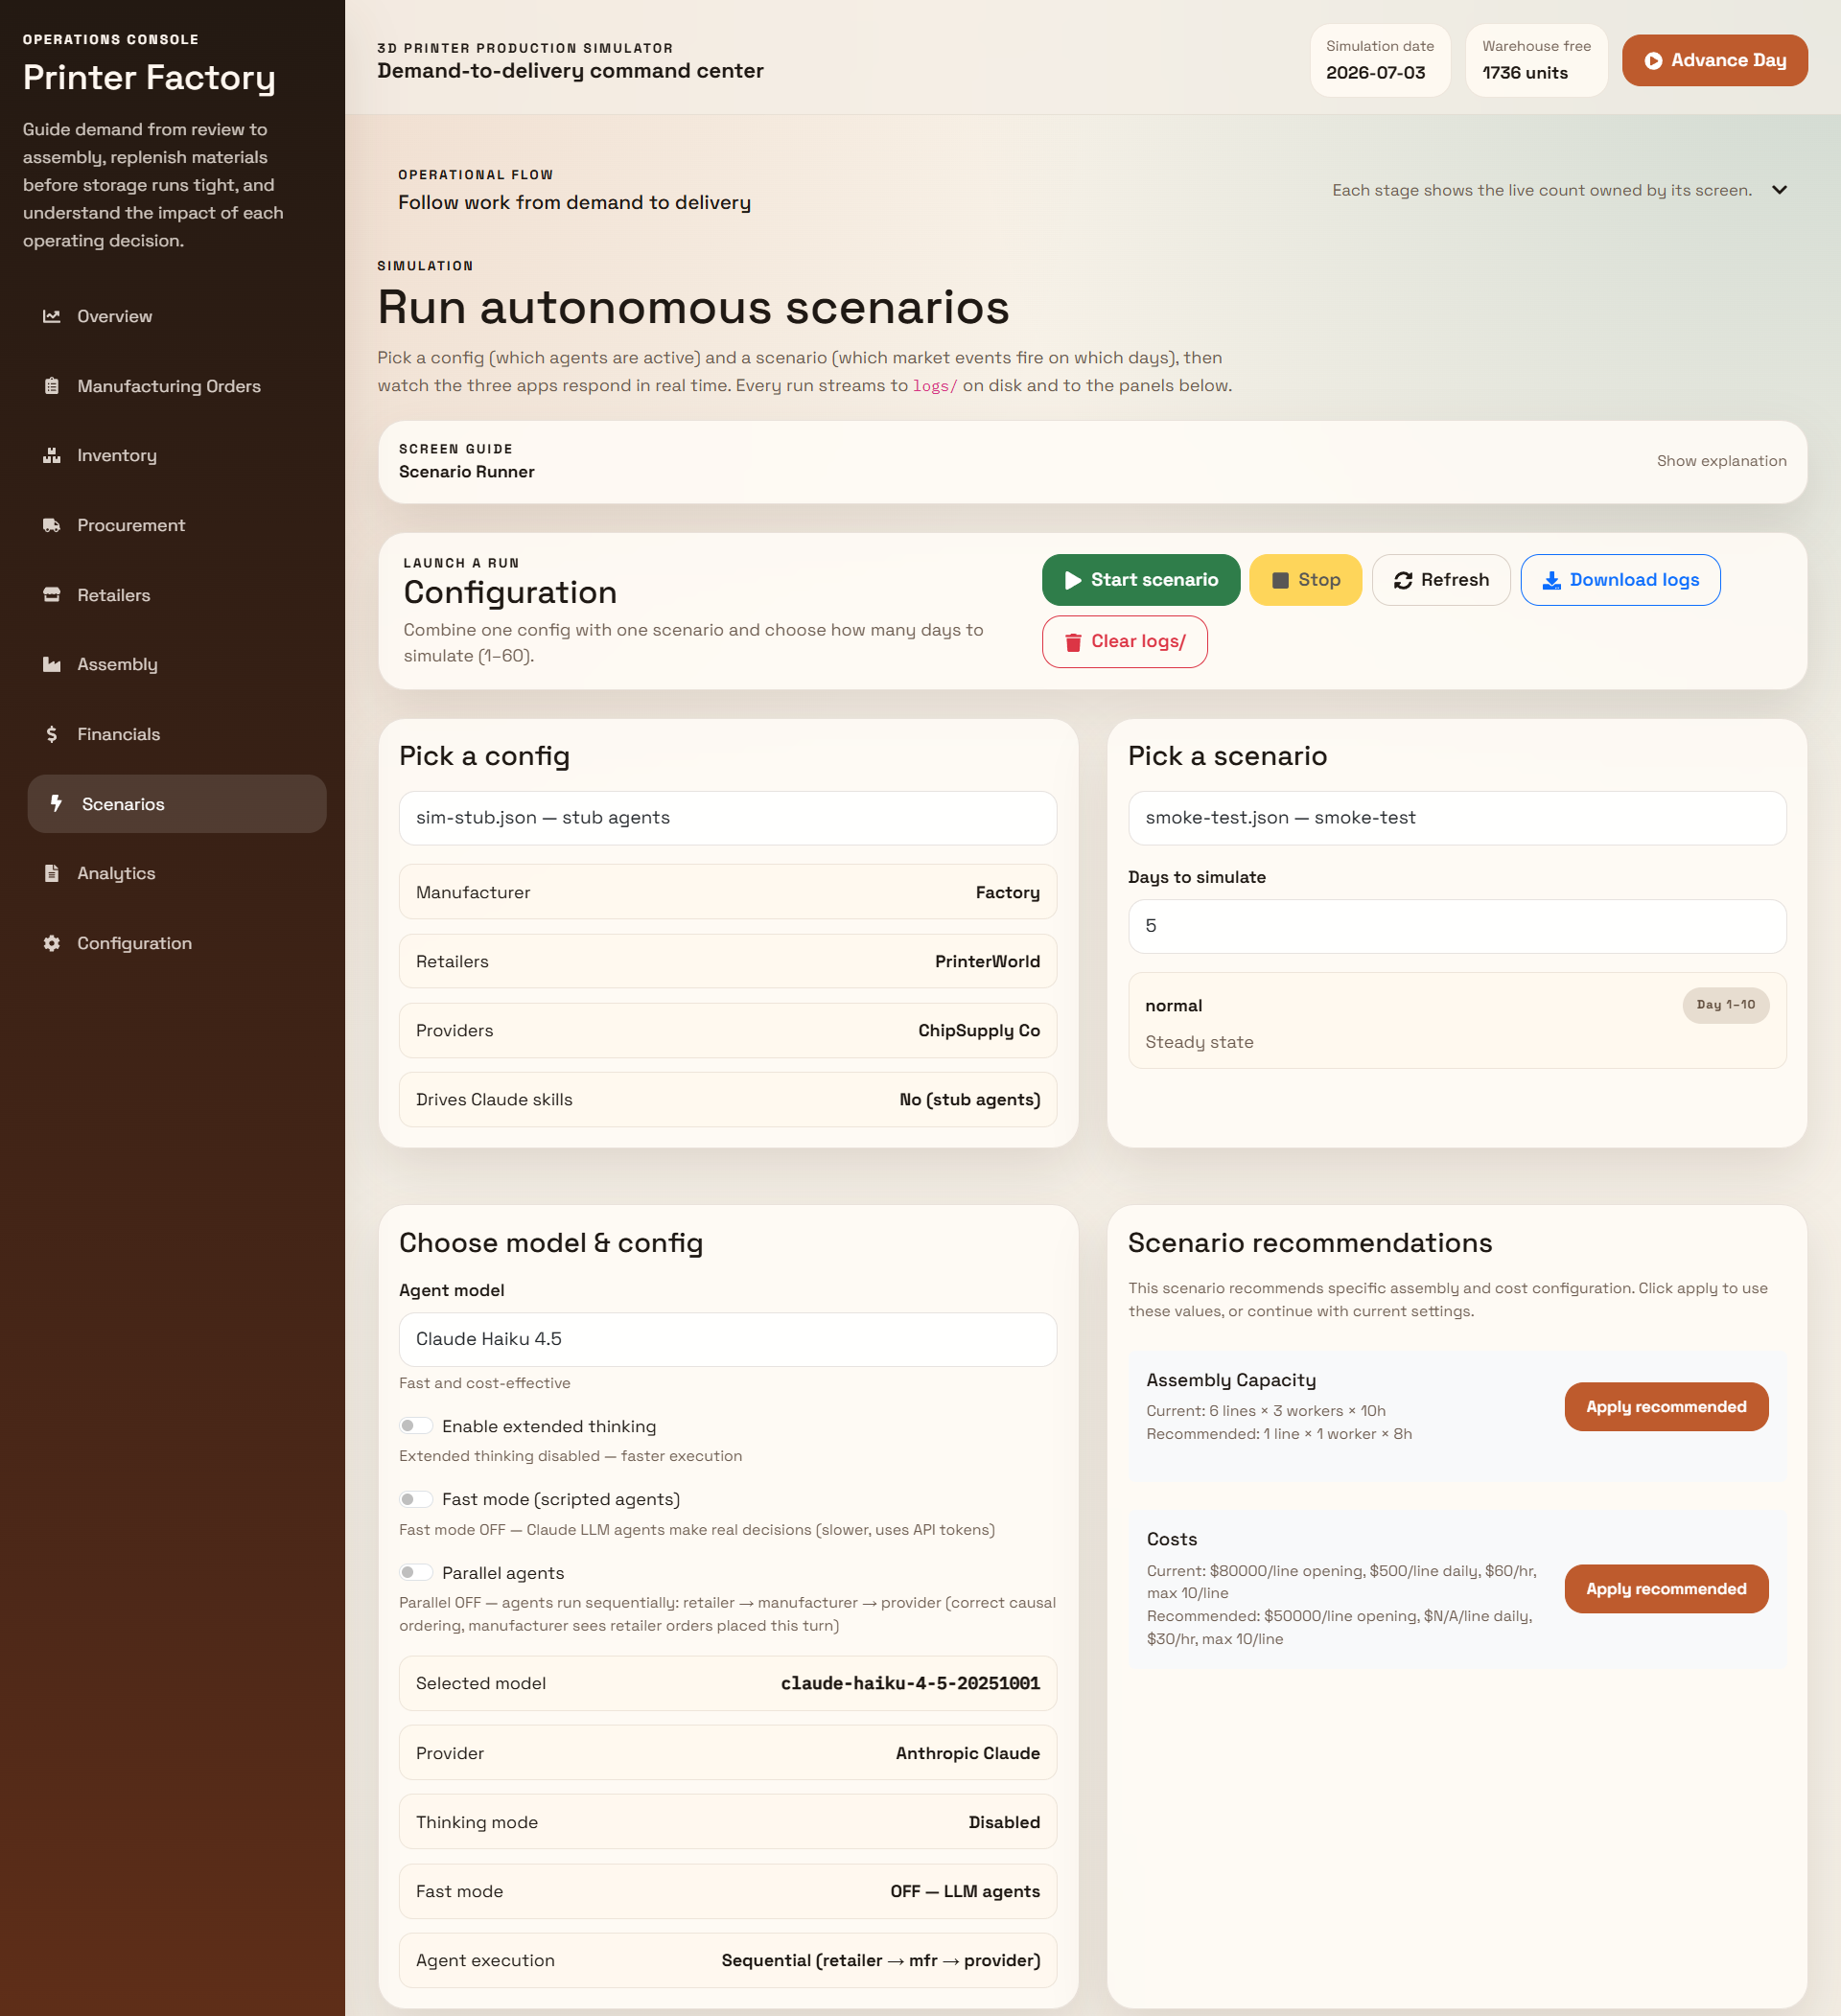
\includegraphics[width=0.45\textwidth]{images/capturas rush/scenarios-HR.png}
\caption{Scenarios page}
\end{figure}

\item \textbf{Scenarios}: the UI launcher for the turn engine. Lets the
operator select a config and scenario file, start or stop a multi-day
run, and tail the per-turn agent logs in the browser without opening a
terminal.

\begin{figure}[H]
\centering
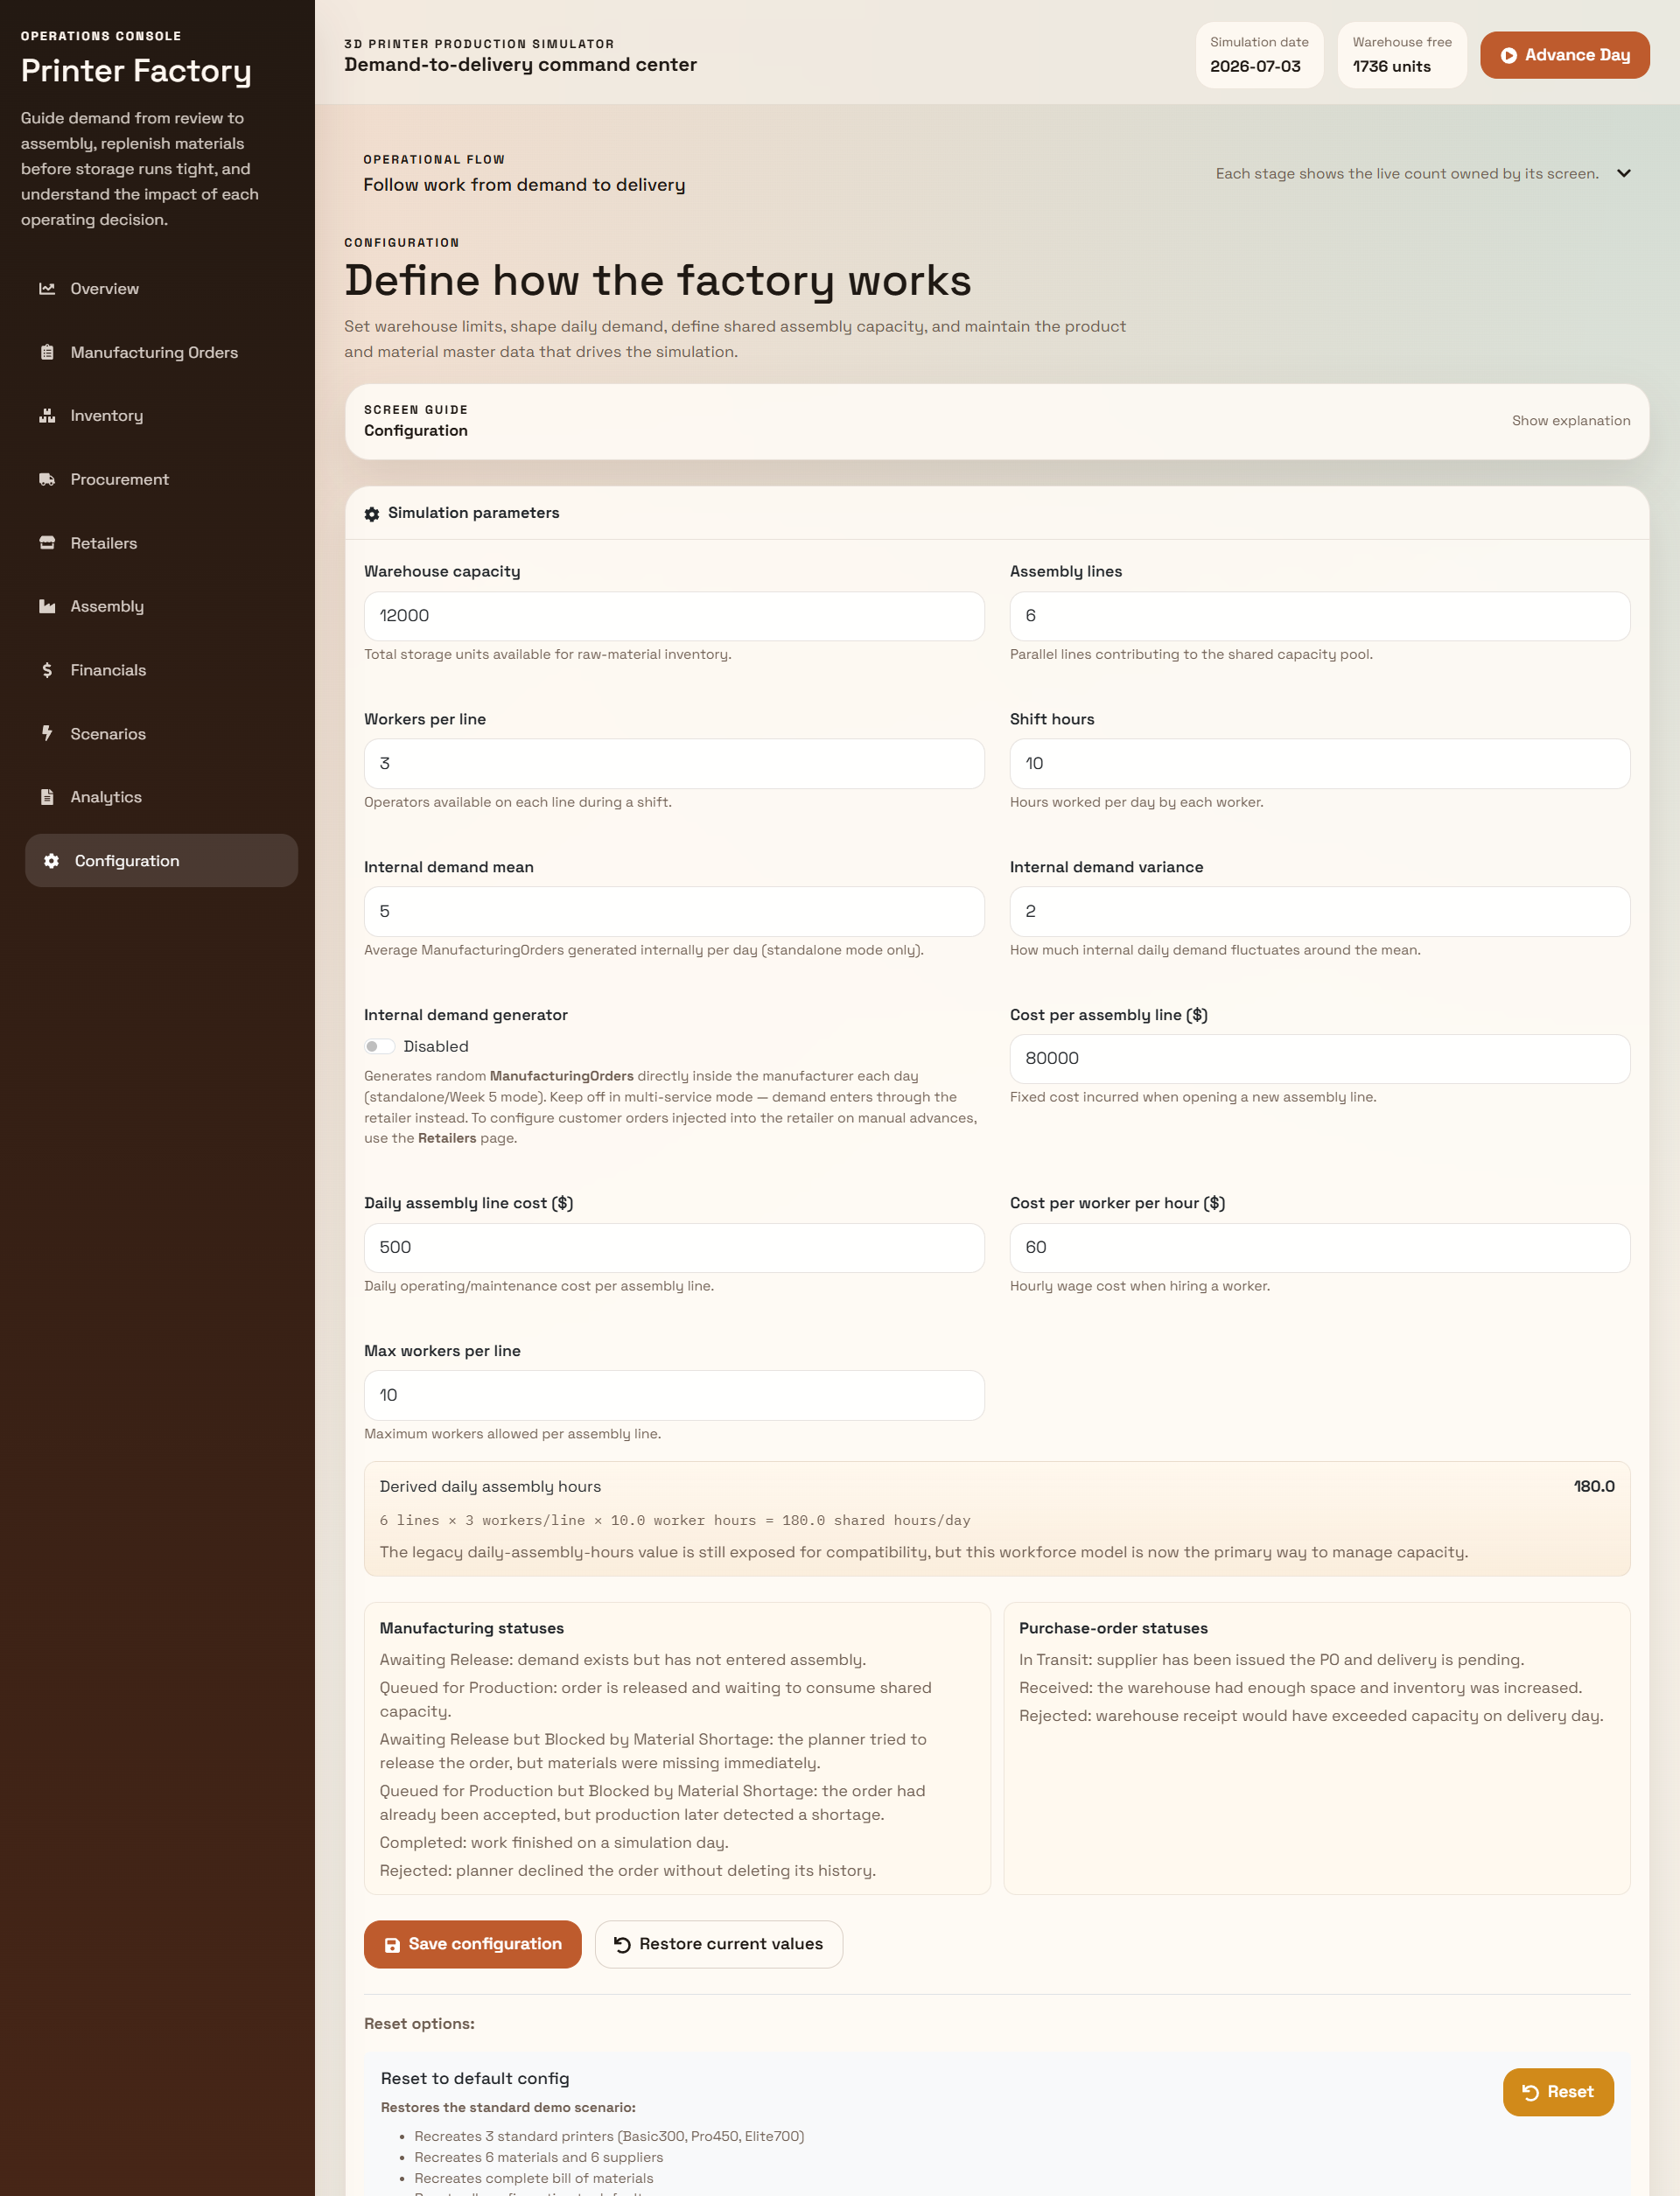
\includegraphics[width=0.45\textwidth]{images/capturas rush/settings-HR.png}
\caption{Settings page}
\end{figure}

\item \textbf{Settings}: simulation configuration: warehouse capacity,
assembly line costs, worker wage rates, and the internal demand
generator toggle. Changes here take effect on the next simulated day.
\end{itemize}


\subsection{Data Models}\label{data-models}

\subsubsection{Provider}\label{provider-chipsupply-co}
\begin{figure}
    \centering
    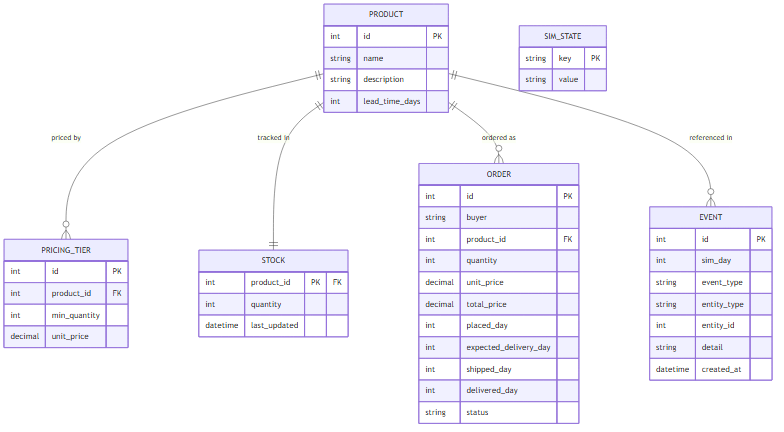
\includegraphics[width=0.85\linewidth]{images/provider.png}
    \caption{Provider data model. Order lifecycle:
\texttt{PENDING\ →\ CONFIRMED\ →\ IN\_PROGRESS\ →\ SHIPPED\ →\ DELIVERED},
with terminal states \texttt{REJECTED} (insufficient stock) and
\texttt{CANCELLED}.}
    \label{fig:placeholder}
\end{figure}

When an order is placed, the stock is immediately
locked so the same units cannot be sold twice. The lock happens at the
moment of ordering, not at the moment the buyer receives the goods.
Every time an order moves from one state to the next, a record is
written to the event log in the same operation, so the audit trail can
never be out of sync with the order state.

\subsubsection{Manufacturer}\label{manufacturer-factory}

\begin{figure}
    \centering
    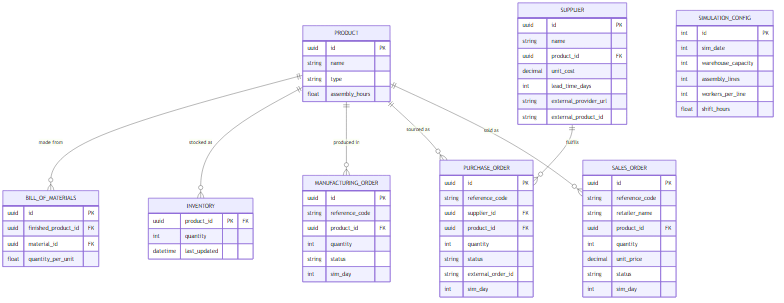
\includegraphics[width=0.85\linewidth]{images/manufacturer.png}
    \caption{Manufacturer data model}
    \label{fig:placeholder}
\end{figure}

The \texttt{Supplier} table gained \texttt{external\_provider\_url} and
\texttt{external\_product\_id} in Week 6. When both are set, the
manufacturer posts purchase orders to the provider's REST API instead of
fulfilling them internally. \texttt{PurchaseOrder.external\_order\_id}
stores the provider-assigned ID for polling.

\subsubsection{Retailer}\label{retailer-printerworld}

\begin{figure}
    \centering
    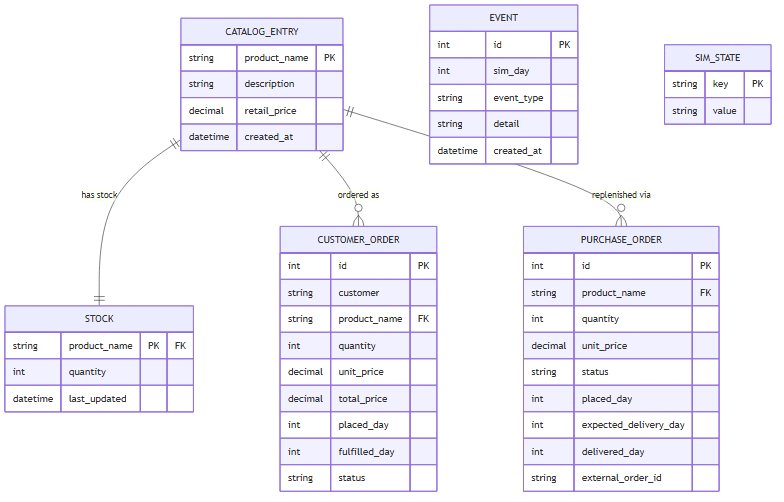
\includegraphics[width=0.85\linewidth]{images/retailer.png}
    \caption{Retailer data model}
    \label{fig:placeholder}
\end{figure}

The retailer keys its catalog by model name string, instead of a shared
ID, since it does not share the manufacturer's product table, this means
that cross-app identity travels as text over HTTP.



\section{Agent Design}\label{b-agent-design}

Three skill files define the role each Claude Code agent plays. Each is
a markdown document passed as a system prompt before the agent's daily
state snapshot.

\subsection{Manufacturer Manager}\label{manufacturer-manager-skillsmanufacturer-manager.md}

The manufacturer agent is the most complex of the three. It manages six
raw materials with different lead times (2--6 days), three assembly
lines with configurable workers, and three finished-product price
points. Its decision framework runs in one pass: assess capacity
backlog, order materials by priority (CRITICAL/FLOOR first, safety stock
second), release pending sales orders, adjust wholesale prices, and
scale workers if queue pressure warrants it.

The key mechanism is the \textbf{proactive ordering strategy}: rather
than waiting for stock to hit zero, the agent is instructed to order
whenever a material is below its floor (30\% of warehouse capacity
divided by number of materials). High-lead-time materials (Aluminum
Frame at 6 days, LCD Screen at 5 days) are ordered at provider maximum
every day they are CRITICAL or LOW, regardless of how much is already in
the pipeline.

\begin{itemize}
  \item \textbf{What the agent is good at:} batching CLI commands, reading capacity metrics, and following the tiered ordering logic when given clear status flags. Capacity scaling is rapid: the agent expanded from 2 lines and 2 workers on day 1 to 6 lines and 10 workers by day 9, reacting to the early backlog fast enough to be fully scaled before Black Friday arrived on day 11.

\begin{figure}[H]
\centering
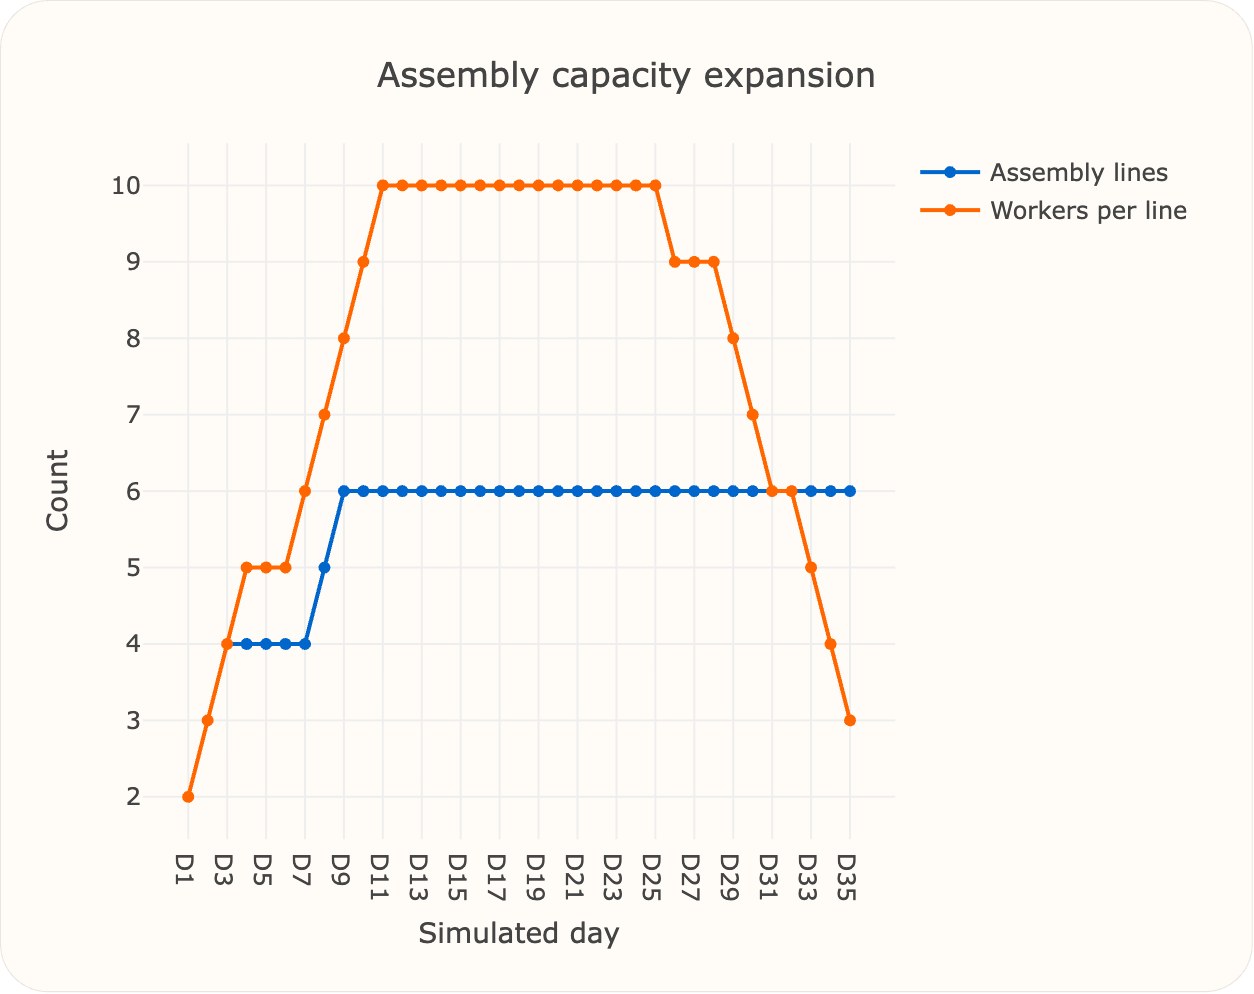
\includegraphics[width=0.6\textwidth]{images/1_Assembly_capacity_expansion.png}
\caption{Number of assembly lines and workers per line across the 35-day run}
\label{fig:assembly-expansion}
\end{figure}

The total capacity chart (Figure~\ref{fig:assembly-expansion}) shows the escalation effect: daily
assembly hours grew from 40h (day 1) to 600h (days 11--25), a 15×
increase driven by both adding lines and adding workers per line
simultaneously. This compounding meant capacity grew much faster than
either lever alone would have produced.

\begin{figure}[H]
\centering
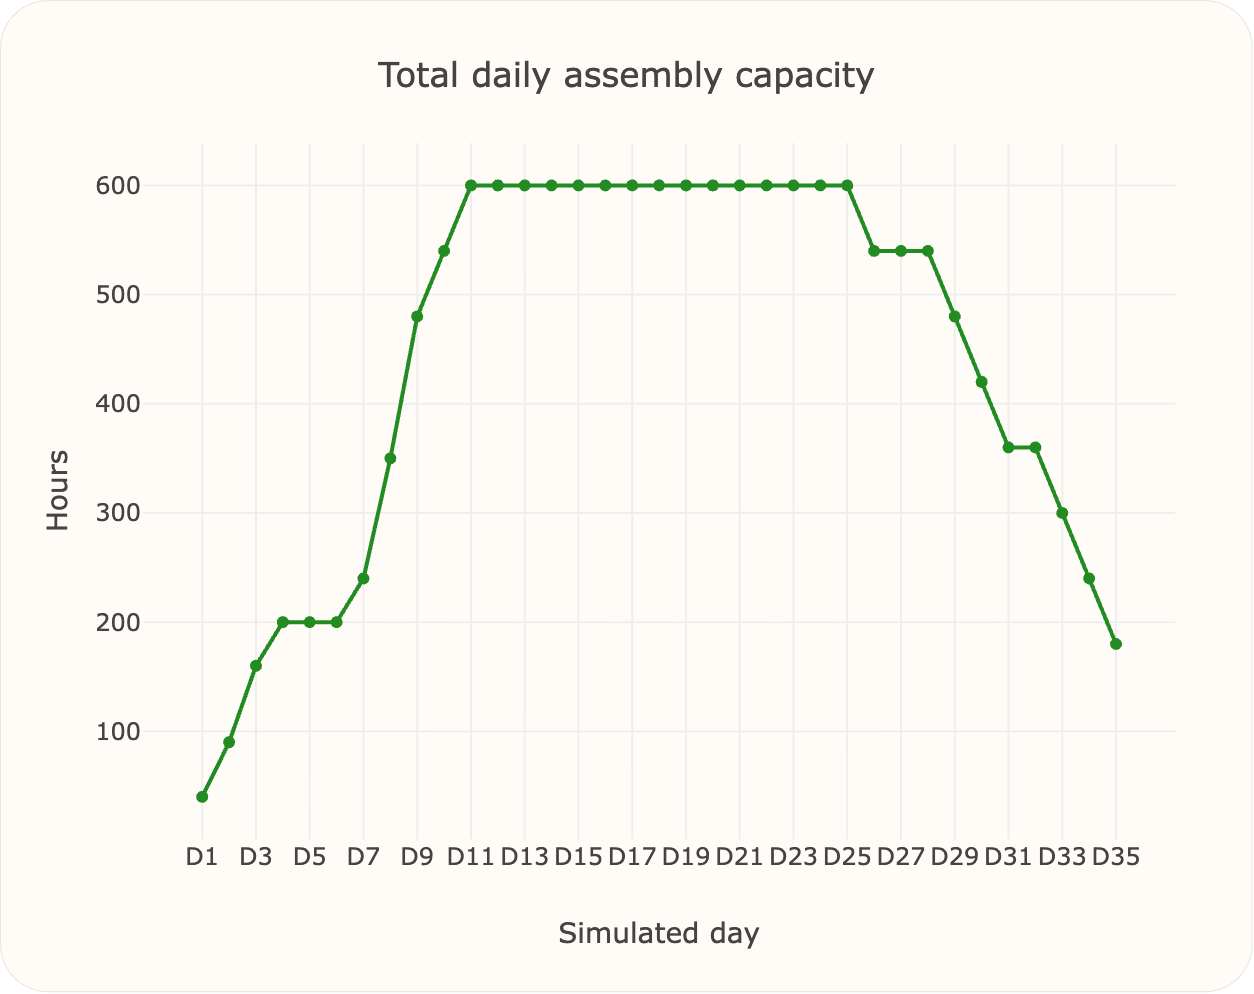
\includegraphics[width=0.6\textwidth]{images/2_Total_daily_assembly_capacity.png}
\caption{Total daily assembly hours (lines × workers × shift hours)}
\end{figure}

\begin{figure}[H]
\centering
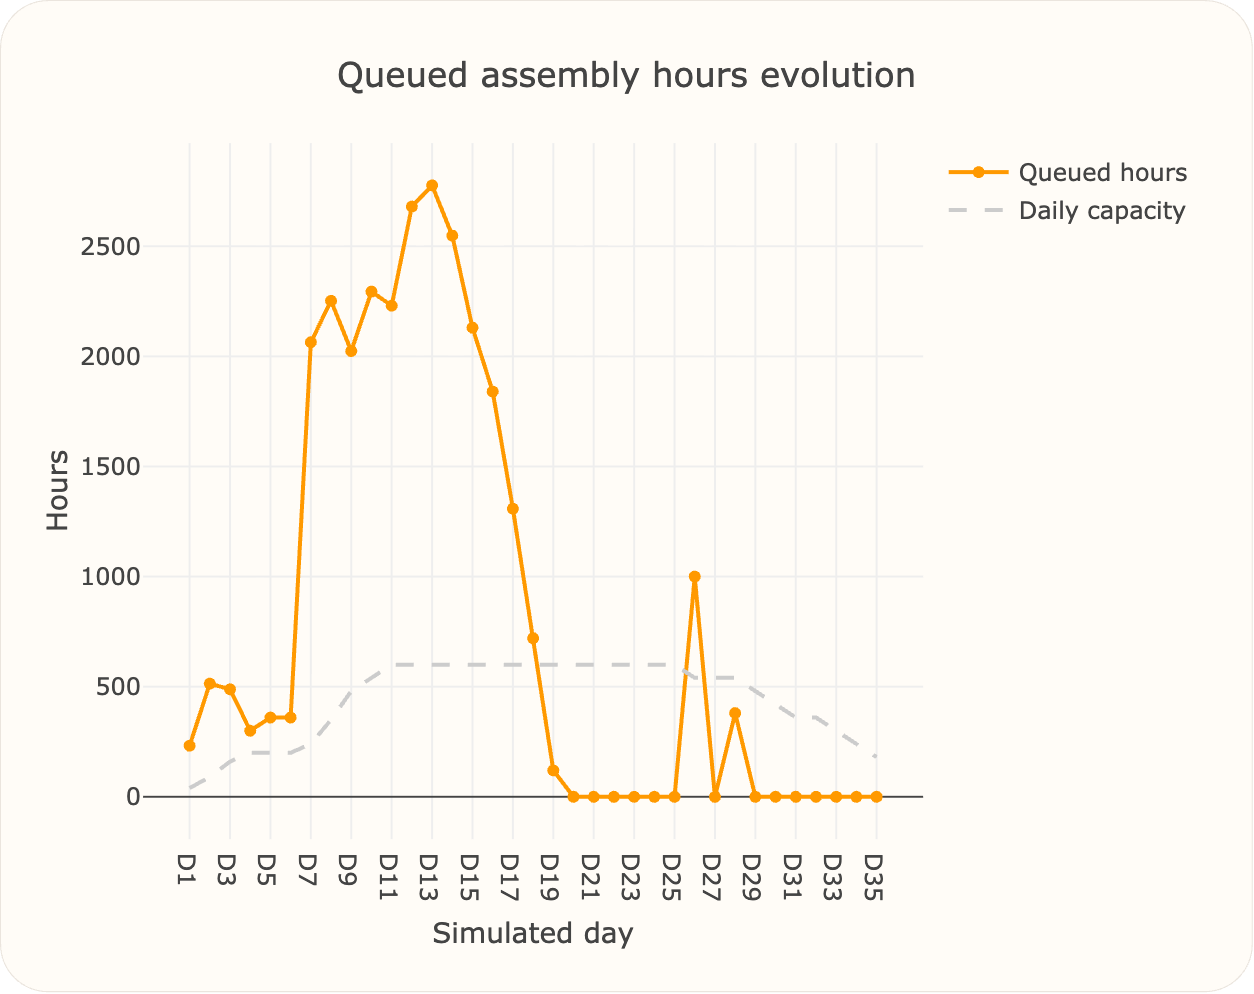
\includegraphics[width=0.6\textwidth]{images/3_Queued_assembly_hours_evolution.png}
\caption{Hours of work queued at the assembly stage each day}
\label{fig:queued-hours}
\end{figure}

The queued hours chart (Figure~\ref{fig:queued-hours}) shows the factory was under sustained
load until day 13 (the end of Black Friday) after which the queue
drained steadily, reaching zero by day 20.

\item \textbf{What the agent is bad at:} The clearest failure was not closing
assembly lines after demand collapsed on day 26, the agent only reduced
workers per line (from 10 down to 3 by day 35), leaving all 6 lines open
and paying fixed costs throughout. It did correctly stop releasing new
production orders from day 26 onwards (the retailer already had 493+
printers against \textasciitilde10 orders/day) and fulfilled 100\% of
customer orders through to day 35, but the idle assembly lines kept
burning fixed costs with no output.

\item \textbf{Skill rewrites:} The PRD-week7 proposed a six-section skeleton. The final file kept that structure and added the following through iterative refinement:

\begin{enumerate}
    \item \textbf{Release PENDING orders first:} Added after the agent logged \emph{``The assembly queue is empty (0.0h), so no production release is possible''} and sat idle for two days with 34+ PENDING orders. Step 0 is placed before all other steps so the empty-queue signal cannot create a blocker before any analysis. Three DO NOT rules were added alongside it: do not treat \texttt{0.0h queued} as a blocker, do not use \texttt{Needed = 0} as a reason to skip releasing, do not treat the stock floor as a release gate.

    \item \textbf{Three-tier ordering system:} The original ``order when below 50\% of starting'' rule was replaced with a tiered structure: Tier 0 = never order EXCESS materials; Tier 1 = order provider max every day for CRITICAL/LOW materials regardless of pipeline size; Tier 2 = demand-weighted safety stock when warehouse has room. This fixed chronic under-ordering of long-lead-time materials during demand surges.

    \item \textbf{Warehouse deadlock detection:} The \texttt{inventory-trash} emergency command and a full deadlock detection workflow were added after runs where incoming purchase orders were rejected because the warehouse was full, which blocked the materials that were needed to release the queued production orders. The skill now checks whether \texttt{current\_usage + pending\_arriving\_today > warehouse\_capacity} and guides the agent to trash surplus materials before the delivery arrives.

    \item \textbf{Assembly line scaling table:} A table mapping \texttt{backlog\_days} and \texttt{demand\_modifier} to hire/fire/open/close decisions replaced the vague ``scale if busy'' guidance. An ROI check was added before any hire or open call.
\end{enumerate}
\end{itemize}

\subsection{\texorpdfstring{Provider Manager
(\texttt{skills/provider-manager.md})}{Provider Manager (skills/provider-manager.md)}}\label{provider-manager-skillsprovider-manager.md}

The provider agent manages six raw material lines for ChipSupply Co.~Its
job each day is to restock products below 50\% of their starting level,
raise prices when stock is below 30\% of starting, lower prices when
stock is above 150\%, and stay within a 15\% daily price change bound.
It receives the same market signal as the other agents and is expected
to restock more aggressively when
\texttt{demand\_modifier\ \textgreater{}\ 1.5}.

\begin{itemize}
  \item \textbf{What the agent is good at:} the restocking decisions are
straightforward, the starting stock targets are explicit in the skill,
so the agent reliably ordered when stock dropped. Most importantly, the
agent kept all component stocks topped up throughout the entire run,
including during the chip shortage (days 14--20), so no material ever
ran out. Because stock never fell below the 30\% threshold that triggers
a price increase, bulk prices correctly stayed flat: Control Board held
at \$25 for all 35 days, consistent with its rules.

\begin{figure}[H]
\centering
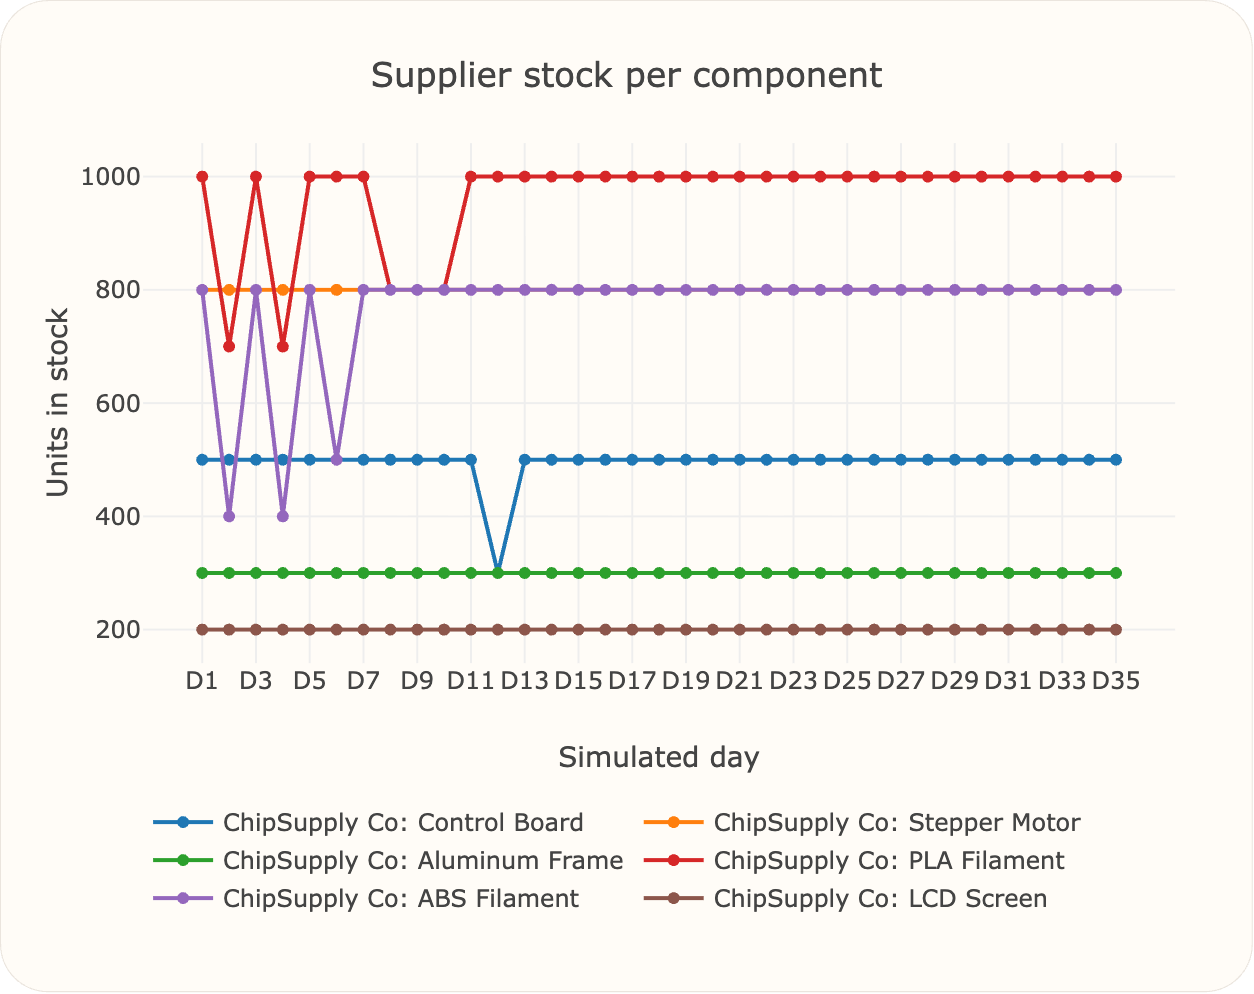
\includegraphics[width=0.6\textwidth]{images/2_Supplier_stock_per_component.png}
\caption{Supplier stock per component}
\end{figure}

    \item \textbf{What the agent is bad at:} Aluminum Frame and ABS Filament
showed erratic price oscillations (roughly \$22--\$38 and \$11--\$24
respectively) that were not clearly tied to stock levels or scenario
events, prices moved up and down without a sustained trend in either
direction. This suggests the agent was reacting to small day-to-day
stock fluctuations rather than following a consistent pricing strategy.

\begin{figure}[H]
\centering
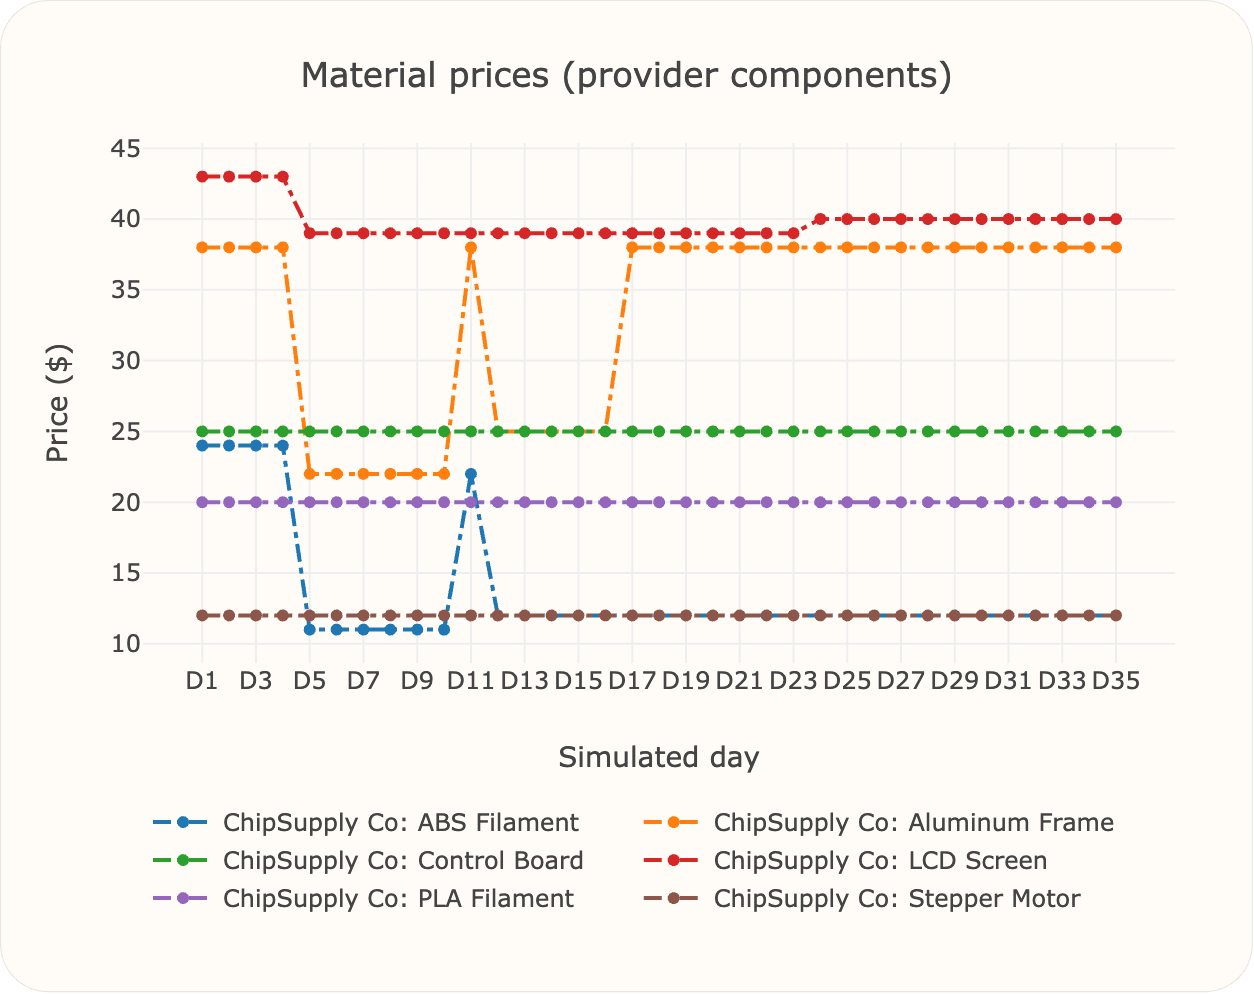
\includegraphics[width=0.6\textwidth]{images/1_Material_prices_provider_components.png}
\caption{Material prices (provider components)}
\end{figure}

\item \textbf{Skill rewrites:}
The week8 brief proposed a minimal five-section template. Key changes applied:

\begin{enumerate}
    \item \textbf{Starting Stock Reference table added:} explicit target quantities per product (Control Board: 500, Stepper Motor: 800, Aluminum Frame: 300, etc.) so the agent has a stable reorder target without calling \texttt{catalog} each day.

    \item \textbf{Restock triggers expanded:} the original ``restock if below 50\% of starting level'' rule was extended with two new conditions: restock earlier when \texttt{lead\_time\_modifier > 1.0} (treating 75\% of target as the reorder point because replenishment will arrive slower), and restock conservatively when \texttt{supply\_modifier < 0.7} (prioritise products tied to pending orders rather than blanket refills).

    \item \textbf{``No price cuts while orders are pending'' rule added:} the original DO NOT only said no >15\% change in one day and no zero stock. A third rule was added to prevent the agent from lowering prices during scarcity while accepted orders were still in progress.

    \item \textbf{\texttt{lead\_time\_modifier} added to Market Signals:} the proposed template only covered \texttt{supply\_modifier < 0.7} and \texttt{demand\_modifier > 1.5}. The current file adds a steady-state band (0.8--1.2 = no action) and \texttt{lead\_time\_modifier > 1.0} as a restock trigger.
\end{enumerate}
\end{itemize}

\subsection{Retail Manager}\label{retail-manager-skillsretail-manager.md}

The retail agent manages PrinterWorld. Each day it fulfills or
backorders pending customer orders, places replenishment orders with the
manufacturer when stock drops below safety thresholds (Basic300: 30
units, Pro450: 15 units, Elite700: 5 units), and adjusts retail prices
5\% up or down based on stock pressure and the active demand signal.

\begin{itemize}
    \item \textbf{What the agent is good at:} fulfillment and backordering logic
was consistent and no customer orders were left in PENDING state at end
of day. The safety stock floor kept replenishment orders arriving even
during quieter periods. On Black Friday (days 11--13) the retailer
fulfilled 82/96/104 orders per day while accumulating 63/59/62
backorders, but the proportion of fulfilled vs backordered was similar
to the pre-surge baseline, in other words, the agent did not perform noticeably worse
under 3× demand than it had during normal days.

    \item \textbf{What the agent is bad at:} After day 26, when the post-holiday
lull cut demand to \textasciitilde10 orders/day, rather than cutting
prices to clear inventory, the retailer's stock for Basic300 and Pro450
kept growing (reaching 840 units by day 35) while retail price fell only
slowly from 4,614 to 3,057 --- still well above what was needed to
stimulate demand at the new lower level.

\begin{figure}[H]
\centering
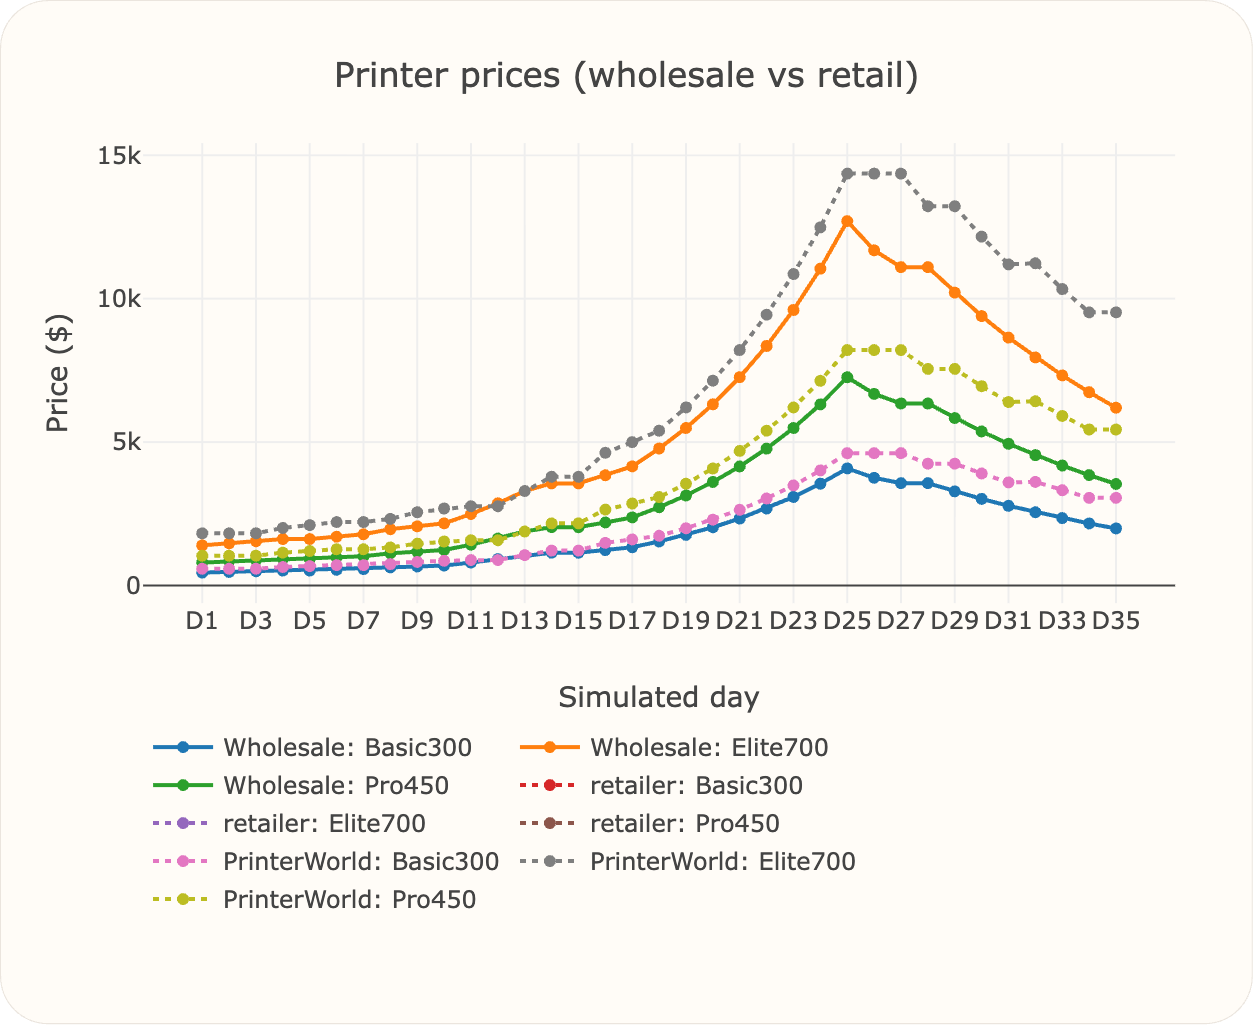
\includegraphics[width=0.6\textwidth]{images/2_Printer_prices.png}
\caption{Basic300 wholesale and retail price per simulated day}
\end{figure}

\begin{figure}[H]
\centering
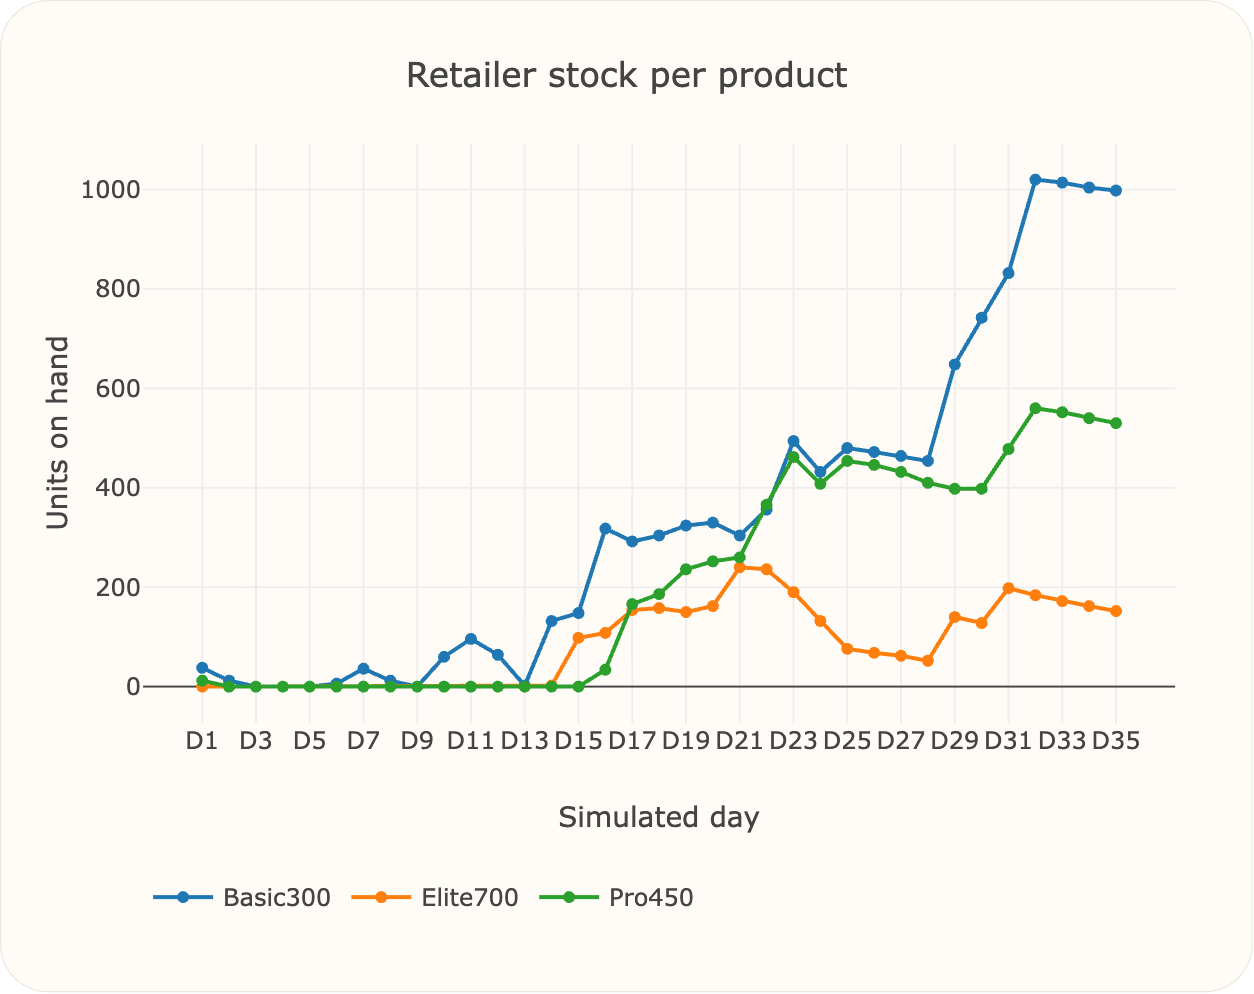
\includegraphics[width=0.6\textwidth]{images/3_Retailer_stock_per_product.png}
\caption{Retailer stock per printer model (Basic300 and Pro450)}
\end{figure}

\item \textbf{Skill rewrites:} The week8 brief proposed a minimal five-section template. Key changes applied:

\begin{enumerate}
    \item \textbf{\texttt{price list} command removed:} the proposed template listed it under Available Commands, but the retailer CLI does not have this command. The agent was calling it and getting errors. Replaced with an explicit DO NOT rule.

    \item \textbf{Safety Stock Targets made explicit:} the proposal used a ``stock < 3 days of recent average demand'' formula to trigger reorders. This was replaced with fixed floor quantities (Basic300: 30 units, Pro450: 15 units, Elite700: 5 units) after the agent produced inconsistent reorder quantities by estimating daily demand differently on each turn.

    \item \textbf{Reorder formula reworked:} the current skill uses the \textbf{Still Short} column from the state table (\texttt{order\_qty = still\_short + safety\_stock\_target - already\_inbound}) and provides a daily demand baseline ($\approx$5/3/2 for Basic300/Pro450/Elite700) so the agent does not have to estimate from history.

    \item \textbf{Pricing model rebuilt:} the proposal had a simple $\pm$5\% rule based on whether stock was above or below a threshold. The current skill uses a two-layer model: first enforce the non-negotiable floor (retail $\geq$ wholesale $\times$ 1.15), then apply a demand-based adjustment table with seven conditions mapping \texttt{demand\_modifier}, backorder count, and \texttt{price\_sensitivity: high} to adjustment percentages (--8\% to +8\%). The 30\% default margin becomes a target rather than a floor, and demand signals override it. This change was driven by the agent raising prices too slowly during Black Friday and cutting them too slowly after the post-holiday lull.

    \item \textbf{Markup floor corrected:} the proposal said ``do not set retail below wholesale + 20\%.'' The actual CLI validation is wholesale $\times$ 1.15 (15\%). The skill was updated to match the real constraint and sets 30\% as the default working target.
\end{enumerate}
\end{itemize}

\section{Simulation Results}\label{c-simulation-results}

Two scenarios were run: holiday-rush (35 days, volatile) and calm-market (35 days, baseline).

\subsection{Scenario Definitions}\label{scenario-definitions}

\begin{table}[H]
\centering
\begin{tabular}{lcccc}
\toprule
\textbf{Event} & \textbf{Days} & \textbf{demand\_modifier} & \textbf{supply\_modifier} & \textbf{lead\_time\_modifier} \\
\midrule
Normal            & 1--10  & 1.0 & 1.0 & 1.0 \\
Black Friday      & 11--13 & 3.0 & 1.0 & 1.0 \\
Chip shortage     & 14--20 & 1.5 & 0.4 & 2.0 \\
Christmas rush    & 18--25 & 2.5 & 0.6 & 1.2 \\
Post-holiday lull & 26--35 & 0.5 & 1.0 & 1.0 \\
\textbf{Calm market} & \textbf{1--20} & \textbf{1.0} & \textbf{1.0} & \textbf{1.0} \\
\bottomrule
\end{tabular}
\end{table}

Days 18--20 have both chip shortage and Christmas active simultaneously.
The engine multiplies demand modifiers (1.5 × 2.5 → 3.75 effective
demand) and takes the minimum supply modifier (0.4), producing the most
stressed window of the entire run.


\subsection{Results \& Interpretation}\label{results-interpretation}

\subsubsection{Did the manufacturer build stock ahead of Black Friday?}

\begin{figure}[H]
\centering
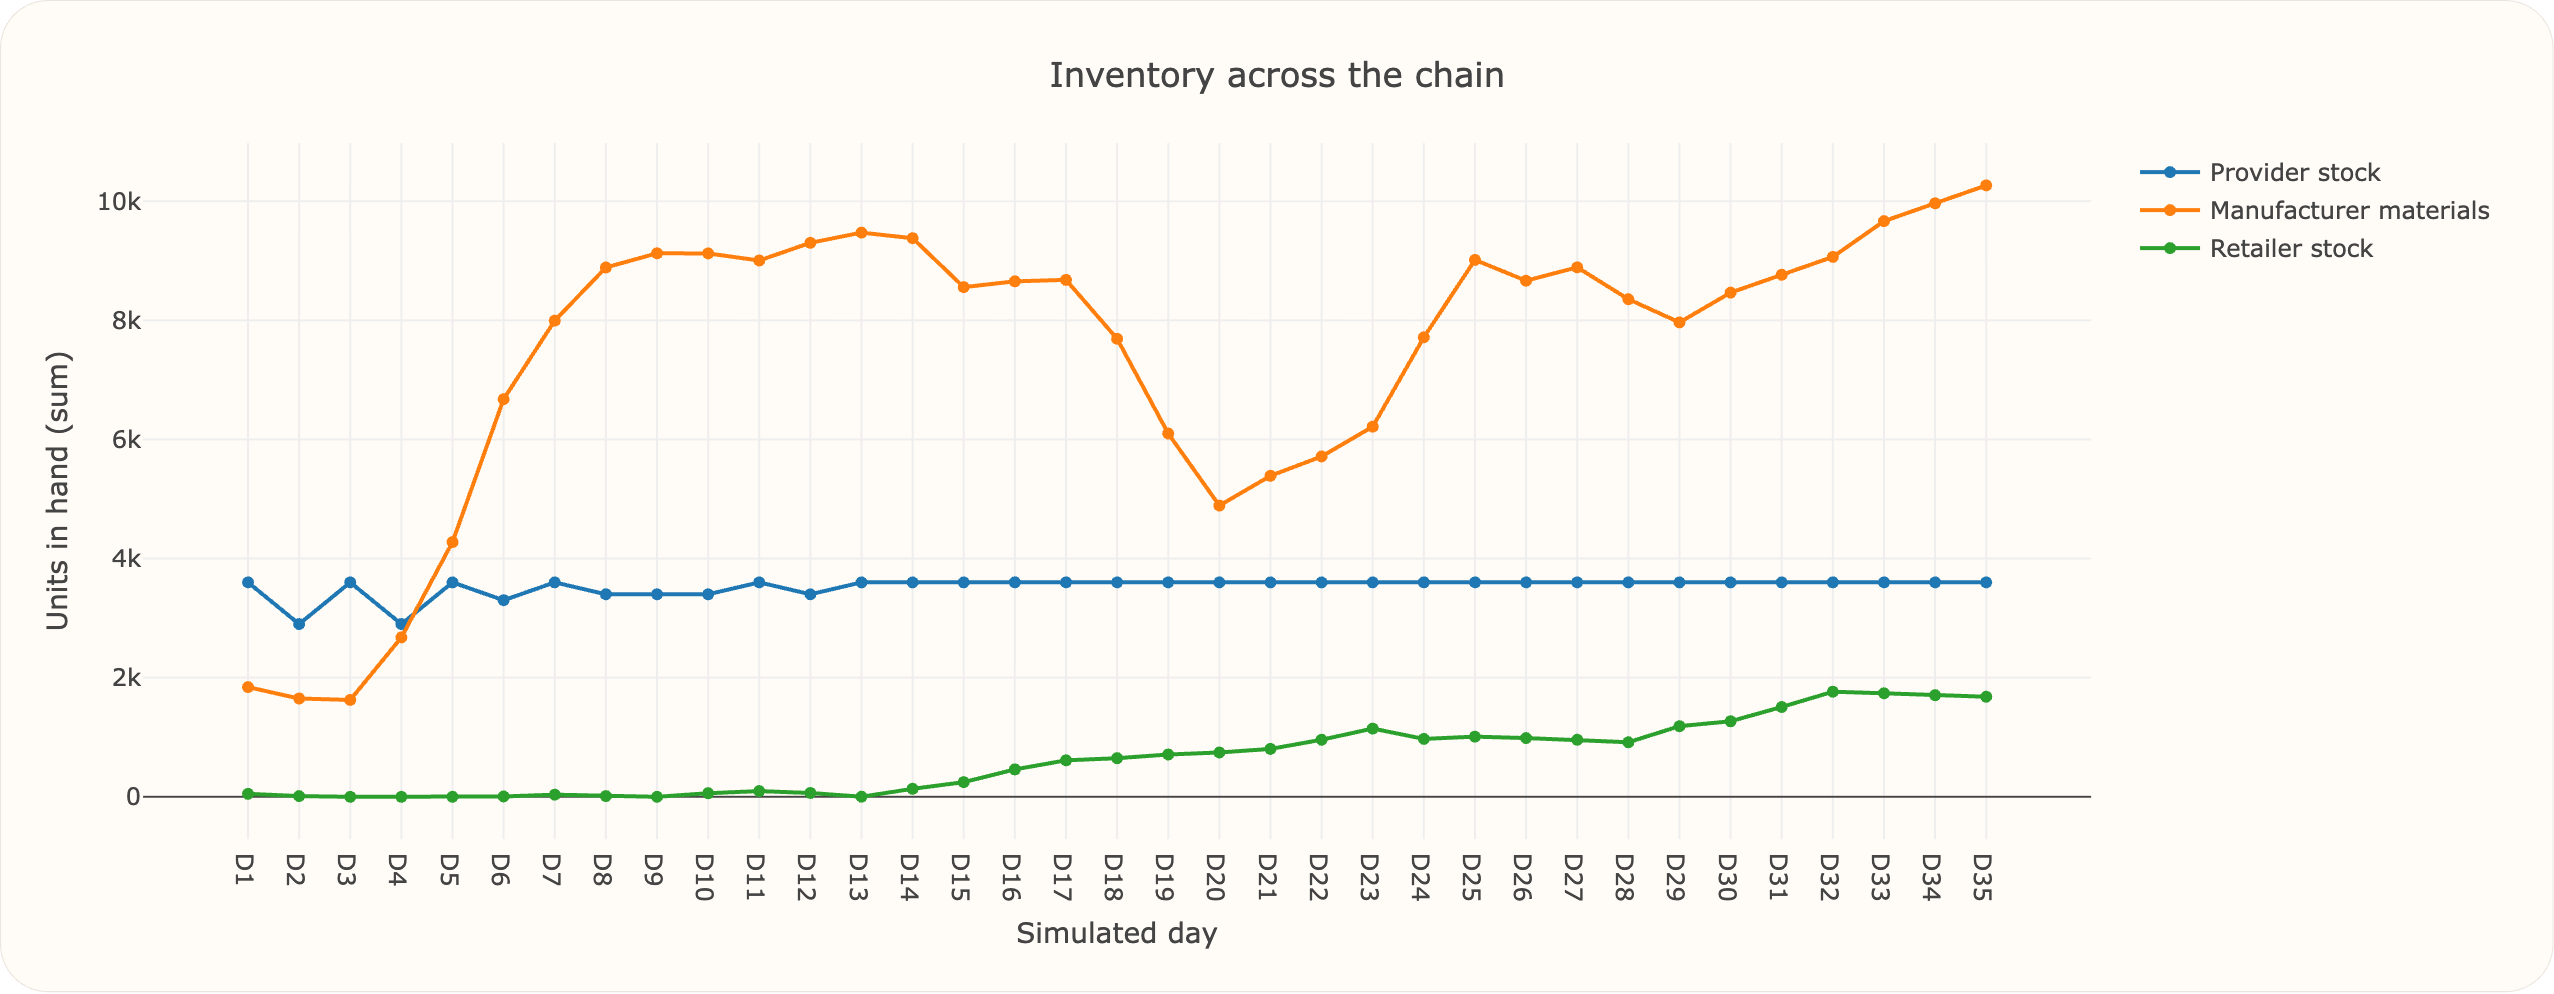
\includegraphics[width=0.6\textwidth]{images/1_Inventory_across_the_chain.png}
\caption{Total stock across all three tiers (chain-wide scale}
\end{figure}

\begin{figure}[H]
\centering
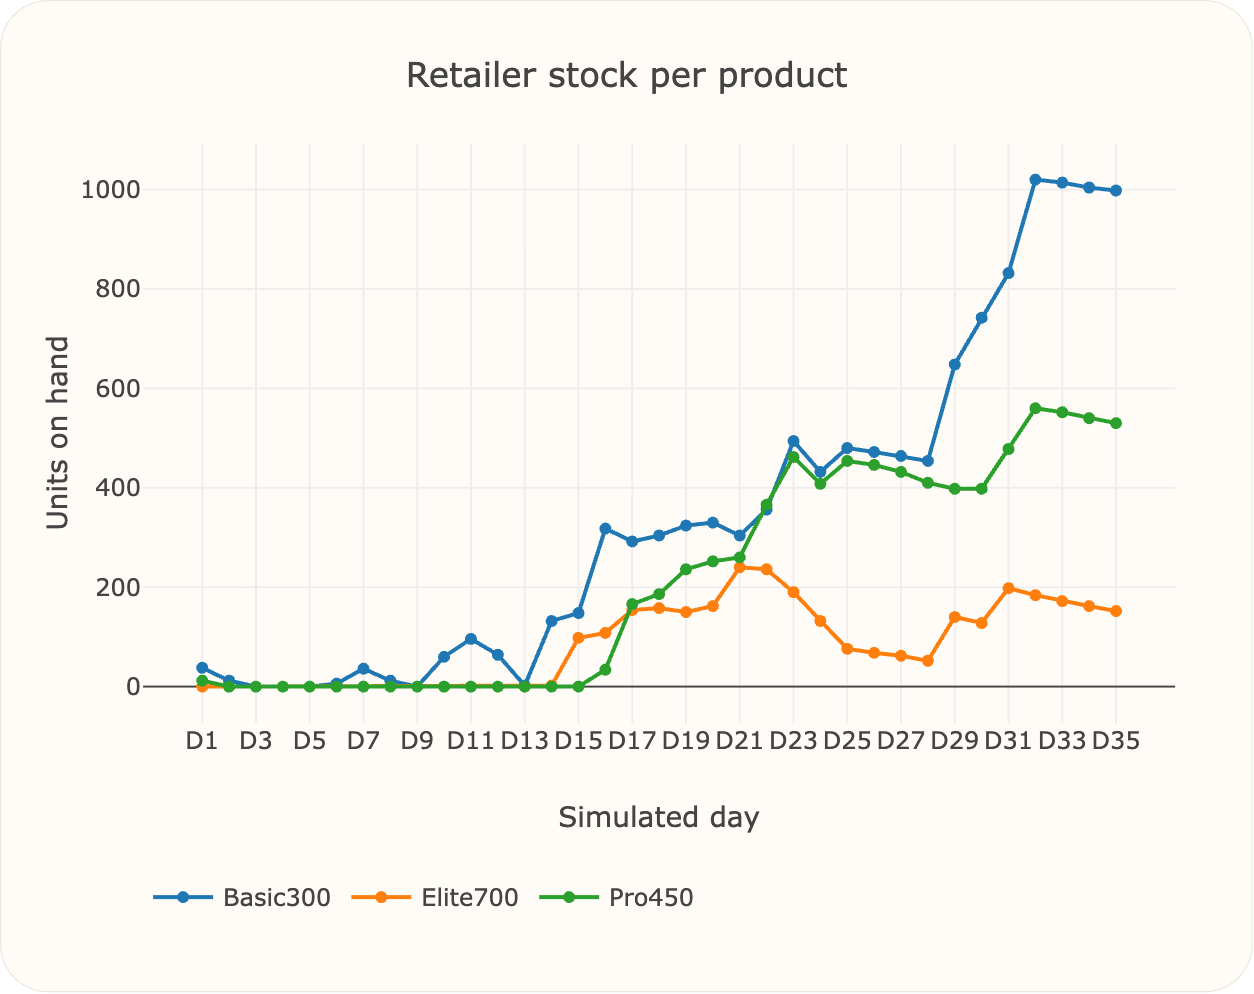
\includegraphics[width=0.6\textwidth]{images/3_Retailer_stock_per_product.png}
\caption{Individual printer counts}
\end{figure}

The retailer's printer stock rose from near zero on day 6 to 30 units on
day 10 and 48 units on day 11, which is the first day of Black Friday.
This build-up was driven by the manufacturer's production queue: active
production orders grew from 7 on day 3 to 38 by day 10, showing the
agent was releasing large batches well in advance. On the materials
side, Control Board inventory climbed from 110 on day 2 to 1,742 by day
9, reflecting aggressive upstream ordering that the agent triggered
because stock was below its floor. The manufacturer did not explicitly
anticipate Black Friday (the market signal does not arrive in advance),
but the proactive reordering rules in the skill produced the right
behaviour anyway.

\subsubsection{When stockouts happened, whose decision was the proximate
cause?}

\begin{figure}[H]
\centering
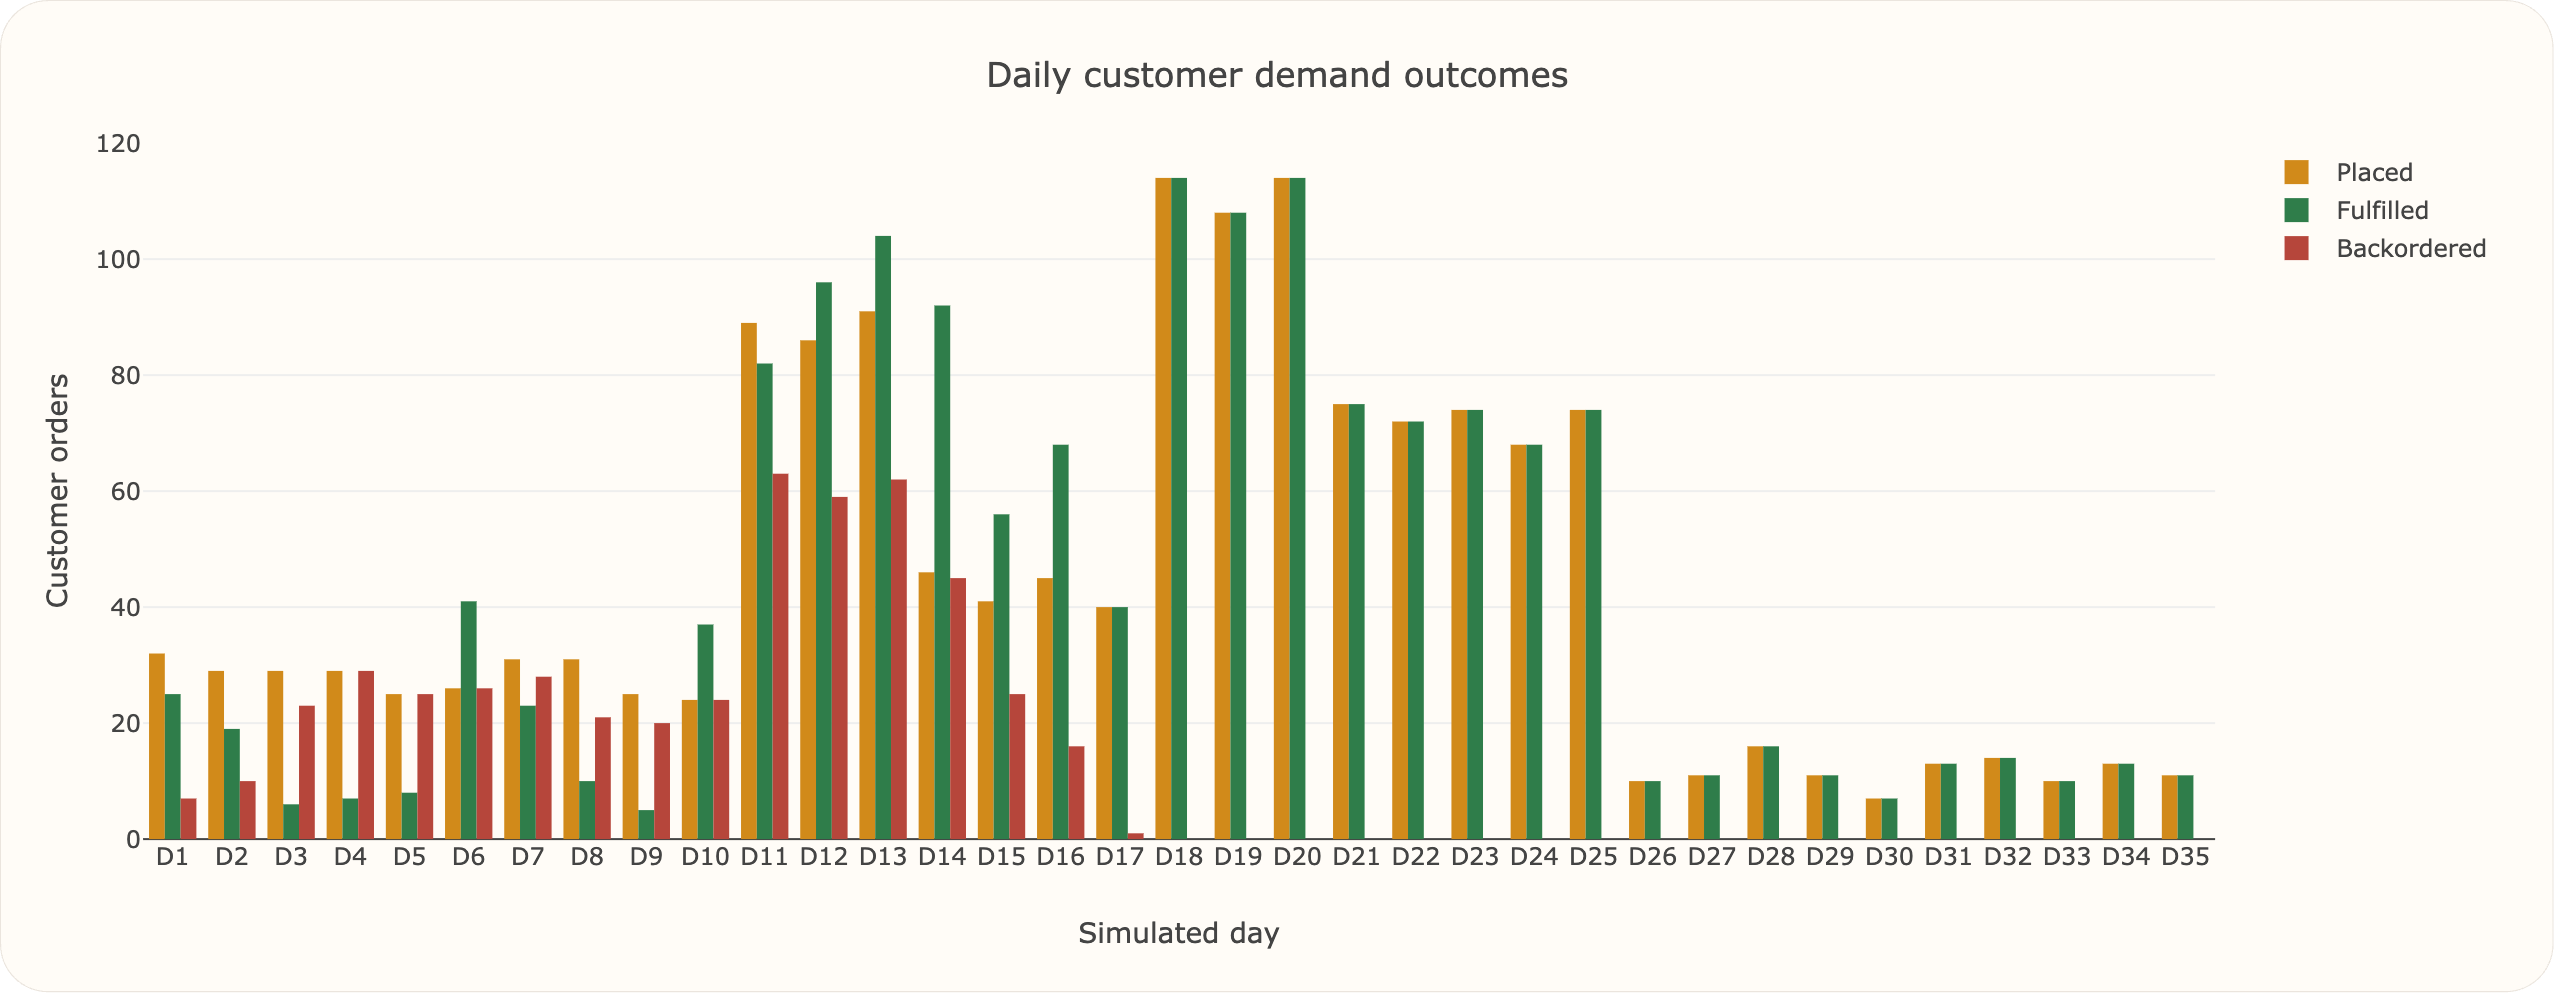
\includegraphics[width=0.9\textwidth]{images/1_Daily_customer_demand_outcomes.png}
\caption{Daily customer demand outcomes}
\end{figure}

\begin{figure}[H]
\centering
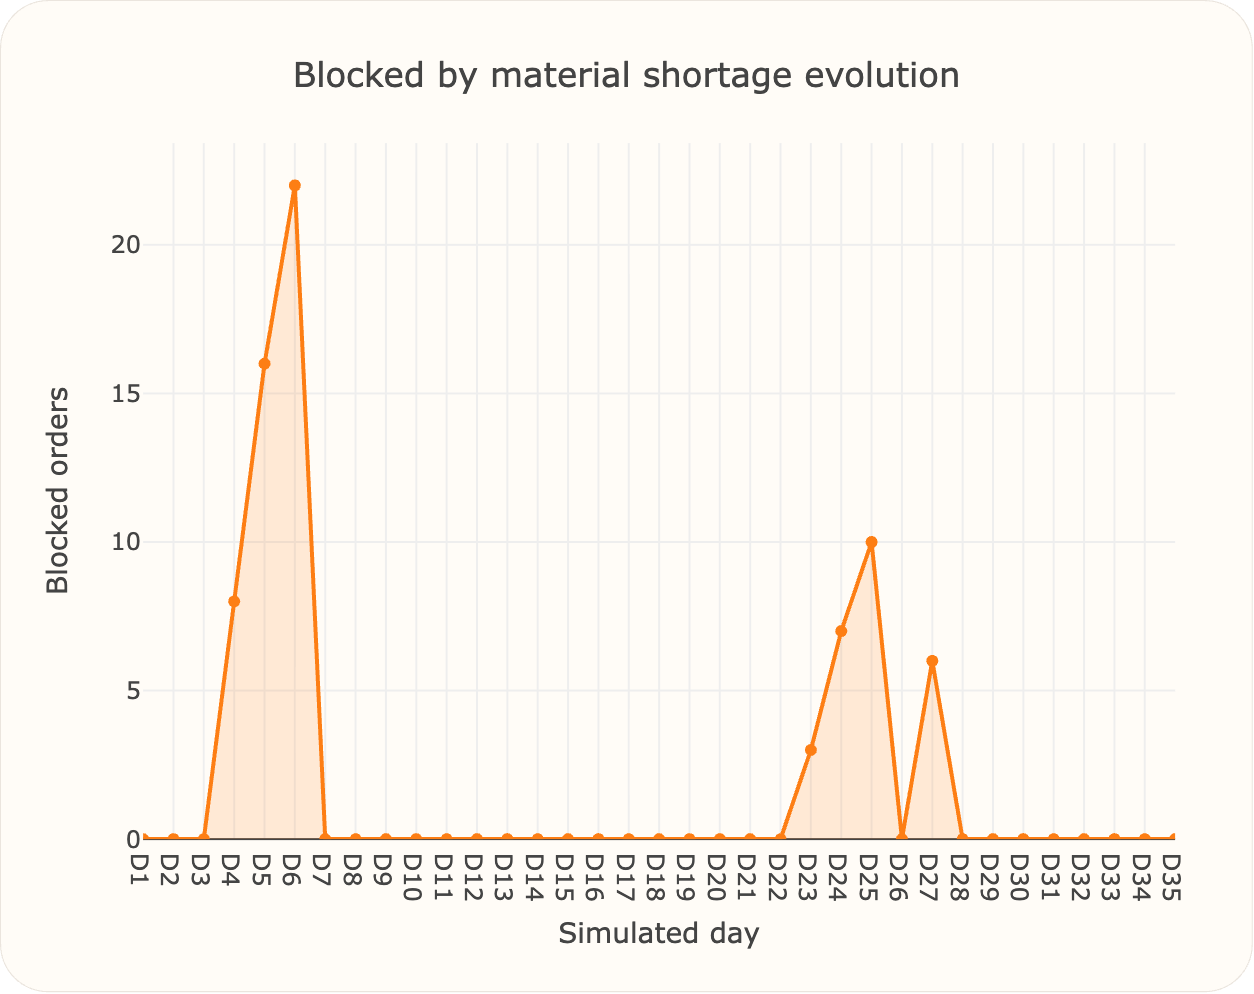
\includegraphics[width=0.6\textwidth]{images/8_Blocked_by_material_shortage_evolution.png}
\caption{Blocked by material shortage evolution}
\end{figure}

The stockout on days 3--6 (four consecutive days at zero retailer stock)
was a throughput bottleneck at the manufacturer rather than a materials
shortage. By day 3 the manufacturer had 545 Control Boards in inventory,
so materials were not the constraint, but blocked orders grew from 8 on
day 4 to 22 on day 6, meaning the assembly queue had more work than it
could complete per turn. The retailer was placing \textasciitilde25
orders per day but printers were not arriving because the production
pipeline needed several days to catch up after the initial stock
depletion. Recovery came on day 6 when 41 units were fulfilled (clearing
accumulated backorders), suggesting the manufacturer's queued production
orders finally cleared. The proximate cause was the retailer starting
with only 25 units and immediately selling through them, with no
same-day production possible.

{\def\LTcaptype{none} % do not increment counter
\begin{longtable}[]{@{}
  >{\raggedright\arraybackslash}p{(\linewidth - 10\tabcolsep) * \real{0.0667}}
  >{\raggedright\arraybackslash}p{(\linewidth - 10\tabcolsep) * \real{0.2000}}
  >{\raggedright\arraybackslash}p{(\linewidth - 10\tabcolsep) * \real{0.2000}}
  >{\raggedright\arraybackslash}p{(\linewidth - 10\tabcolsep) * \real{0.1467}}
  >{\raggedright\arraybackslash}p{(\linewidth - 10\tabcolsep) * \real{0.1733}}
  >{\raggedright\arraybackslash}p{(\linewidth - 10\tabcolsep) * \real{0.2133}}@{}}
\toprule\noalign{}
\begin{minipage}[b]{\linewidth}\raggedright
Day
\end{minipage} & \begin{minipage}[b]{\linewidth}\raggedright
Retailer stock
\end{minipage} & \begin{minipage}[b]{\linewidth}\raggedright
Orders placed
\end{minipage} & \begin{minipage}[b]{\linewidth}\raggedright
Fulfilled
\end{minipage} & \begin{minipage}[b]{\linewidth}\raggedright
Backordered
\end{minipage} & \begin{minipage}[b]{\linewidth}\raggedright
Blocked (mfr)
\end{minipage} \\
\midrule\noalign{}
\endhead
\bottomrule\noalign{}
\endlastfoot
1 & 25 & 32 & 25 & 7 & 0 \\
2 & 6 & 29 & 19 & 10 & 0 \\
3 & 0 & 29 & 6 & 23 & 0 \\
4 & 0 & 29 & 7 & 29 & 8 \\
5 & 0 & 25 & 8 & 25 & 16 \\
6 & 3 & 26 & 41 & 26 & 22 \\
\end{longtable}
}

\subsubsection{Did prices stabilise or oscillate?}

\begin{figure}[H]
\centering
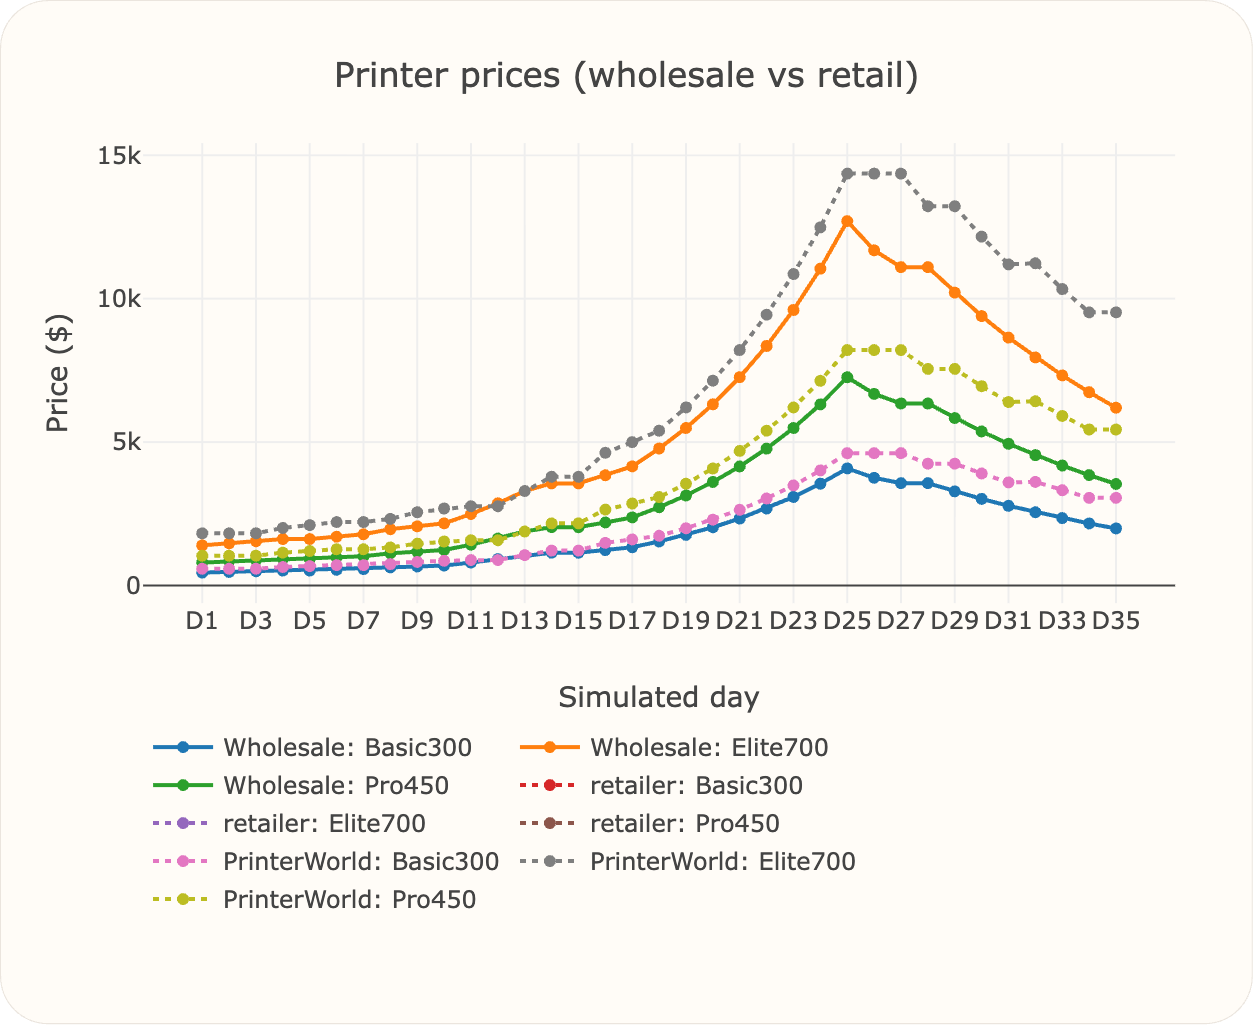
\includegraphics[width=0.6\textwidth]{images/2_Printer_prices.png}
\caption{Printer prices}
\end{figure}

Both wholesale and retail prices moved monotonically with only 3
direction changes across the entire run without any oscillation.
Basic300 wholesale rose steadily from 450 on day 1 to 4,082 on day 25
(the Christmas rush peak), then fell gradually to 1,990 by day 35. The
retail price lagged slightly behind: it stayed at 585 for three days
while wholesale had already risen, and held at 4,614 for three extra
days into the post-holiday lull before catching up. The only genuine
price swing was in the provider's Control Board tier-1 price, which
jumped from 55 to 220 on day 17 and back to 55 within three days --- but
this was the provider agent overcorrecting, and it did not cause the
printer prices to oscillate because the manufacturer's pricing rules
smooth out single-day input cost spikes.

{\def\LTcaptype{none} % do not increment counter
\begin{longtable}[]{@{}lllll@{}}
\toprule\noalign{}
Day & Event & Basic300 wholesale & Basic300 retail & CB tier-1 \\
\midrule\noalign{}
\endhead
\bottomrule\noalign{}
\endlastfoot
1 & normal & 450 & 585 & 40 \\
3 & normal & 496 & 585 & 55 \\
10 & normal & 697 & 862 & 55 \\
16 & chip shortage & 1,236 & 1,487 & 55 \\
17 & chip shortage & 1,334 & 1,606 & \textbf{220} \\
18 & chip + christmas & 1,535 & 1,735 & 110 \\
20 & chip + christmas & 2,029 & 2,294 & 55 \\
25 & christmas peak & \textbf{4,082} & \textbf{4,614} & 55 \\
26 & post-holiday lull & 3,755 & 4,614 & 55 \\
29 & post-holiday lull & 3,282 & 4,247 & 55 \\
35 & post-holiday lull & 1,990 & 3,057 & 55 \\
\end{longtable}
}

\subsubsection{Can you identify a bullwhip moment?}

\begin{figure}[H]
\centering
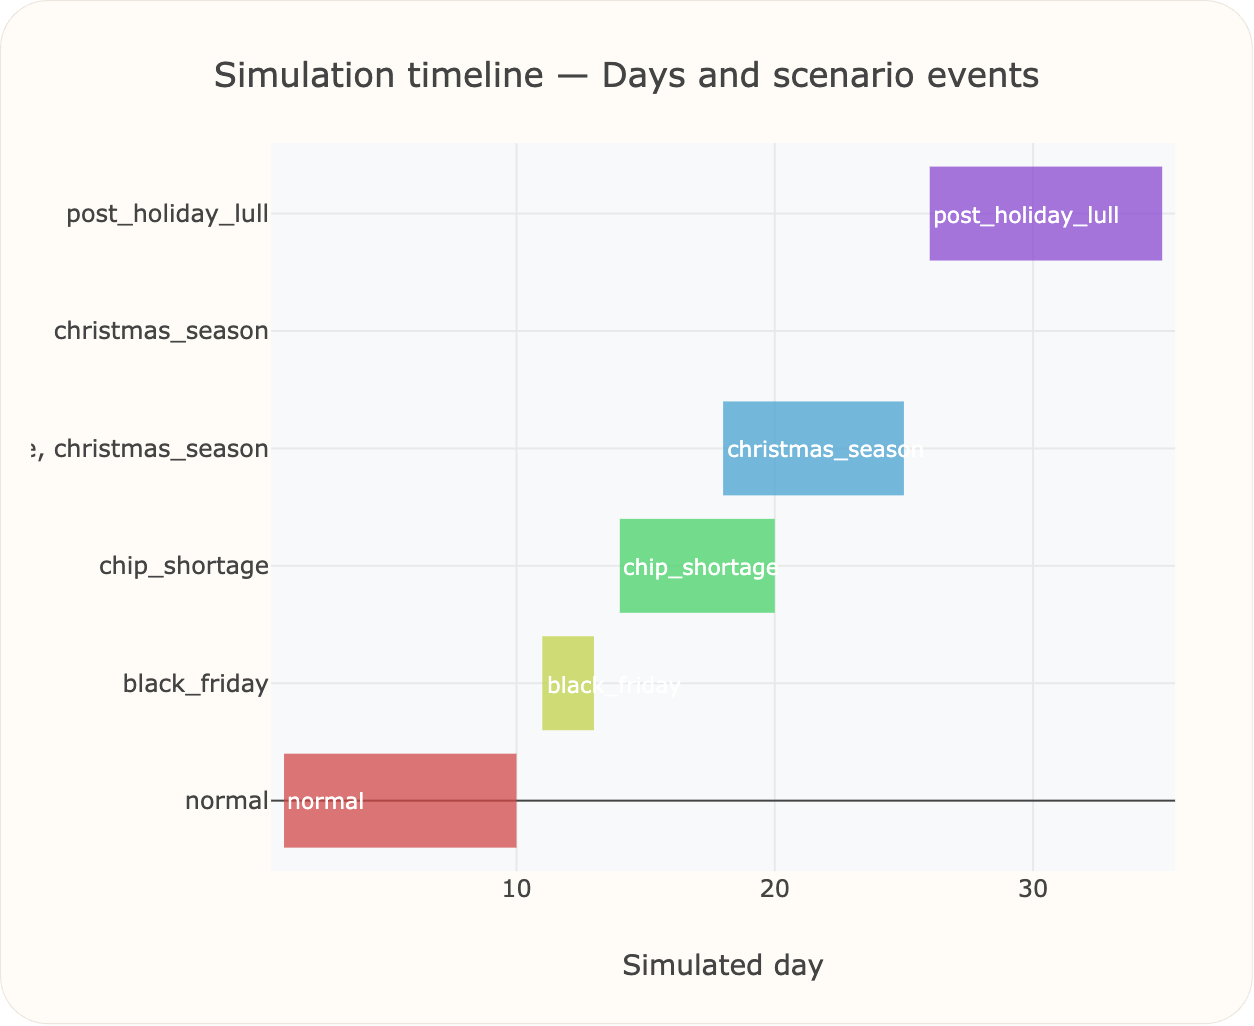
\includegraphics[width=0.6\textwidth]{images/3_Scenario_events_timeline.png}
\caption{Active scenario events by day (demand and supply modifiers in effect)}
\end{figure}

There is no bullwhip moment in this run. Looking at the actual
manufacturer-to-provider purchase orders, the manufacturer's ordering
was driven by its own internal stock floor targets rather than by retail
demand signals. The largest upstream orders (2,500--2,800 units/day)
happened during days 1--4 when retail demand was only
\textasciitilde29/day, because the manufacturer was building its initial
stock buffer. During Black Friday (days 11--13) when retail orders
tripled to \textasciitilde89/day, manufacturer orders to the provider
stayed flat at 2,100--2,300 not showing any amplification. During the
Christmas rush (days 18--25), manufacturer orders actually declined to
600--1,800/day because it was drawing down existing inventory instead of
ordering more. The post-holiday overstock (retailer stock growing from
493 to 840 units after day 26) showed a pipeline inertia, which means
that printers already in production kept arriving after demand
collapsed, not a bullwhip amplification across tiers.

\subsubsection{Financial performance}

\begin{figure}[H]
\centering
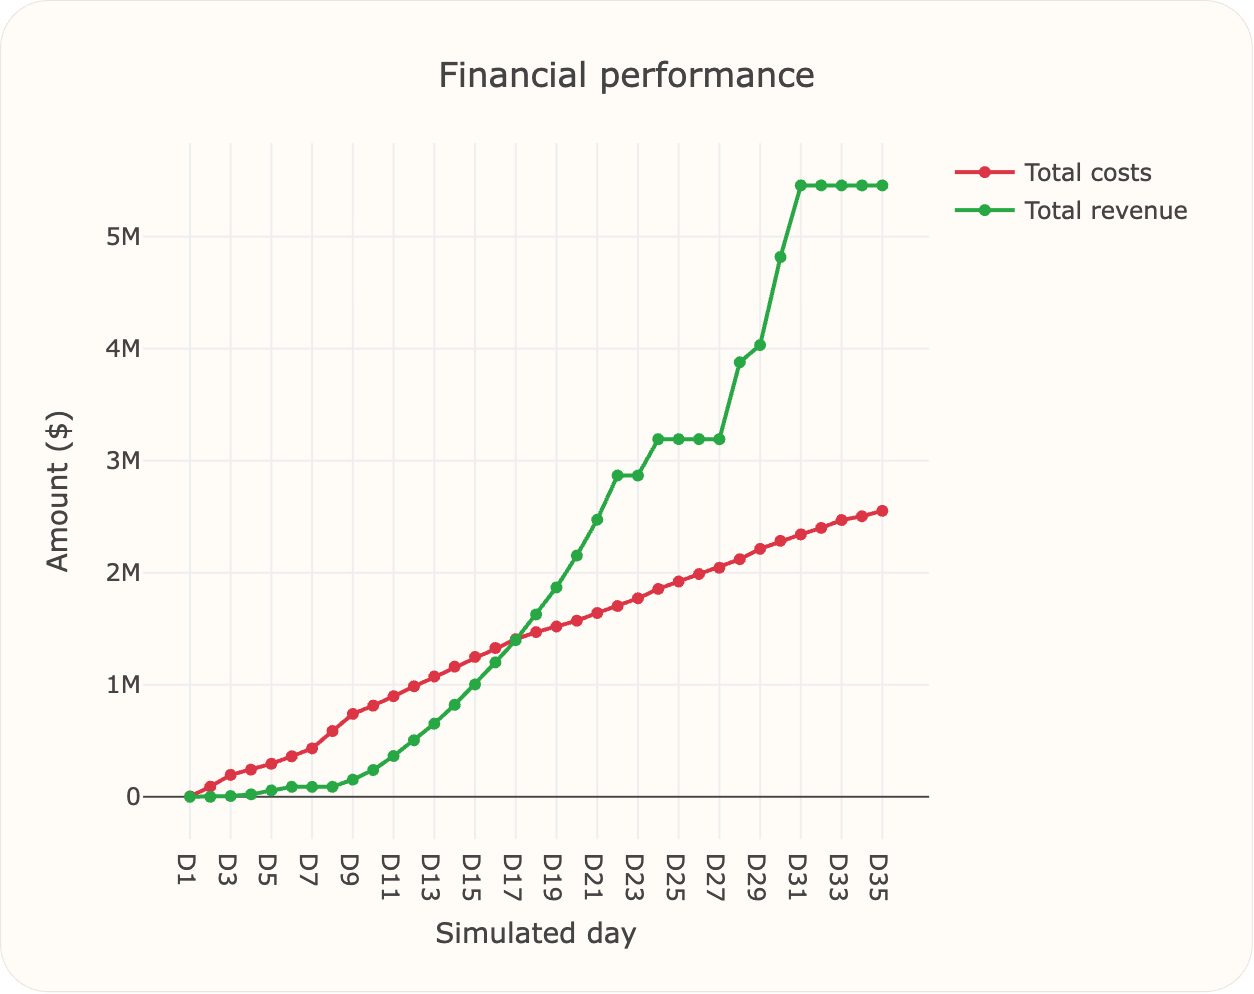
\includegraphics[width=0.6\textwidth]{images/5_Financial_performance.png}
\caption{Financial performance}
\end{figure}

\begin{figure}[H]
\centering
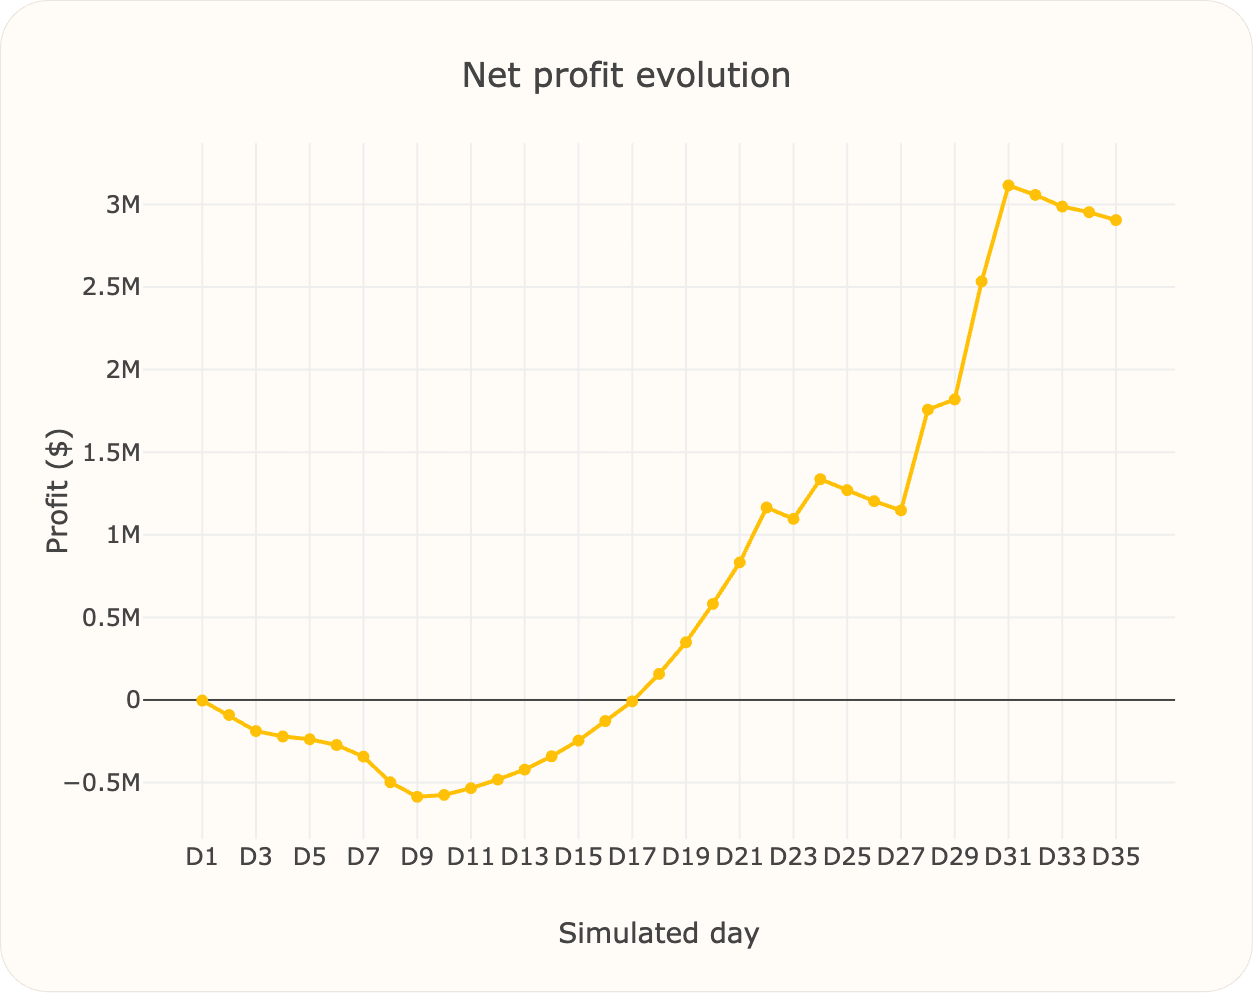
\includegraphics[width=0.6\textwidth]{images/6_Net_profit_evolution.png}
\caption{Net profit evolution}
\end{figure}

Costs increased in a very linear way throughout the run, as the fixed
assembly line costs accrued every day regardless of output. Revenues, by
contrast, were near zero until day 8, after which they grew steeply as
finished printers started shipping to the retailer. The factory stopped
running at a loss on day 17, when cumulative revenues finally surpassed
cumulative costs. From day 31 onwards revenues stabilised as the
post-holiday lull reduced demand and the manufacturer's production
effectively stopped.



\subsection{Scenario Comparison between Holiday Rush Scenario and
Calm Market
Scenario}\label{scenario-comparison-between-holiday-rush-scenario-and-calm-market-scenario}

\begin{figure}[H]
\centering
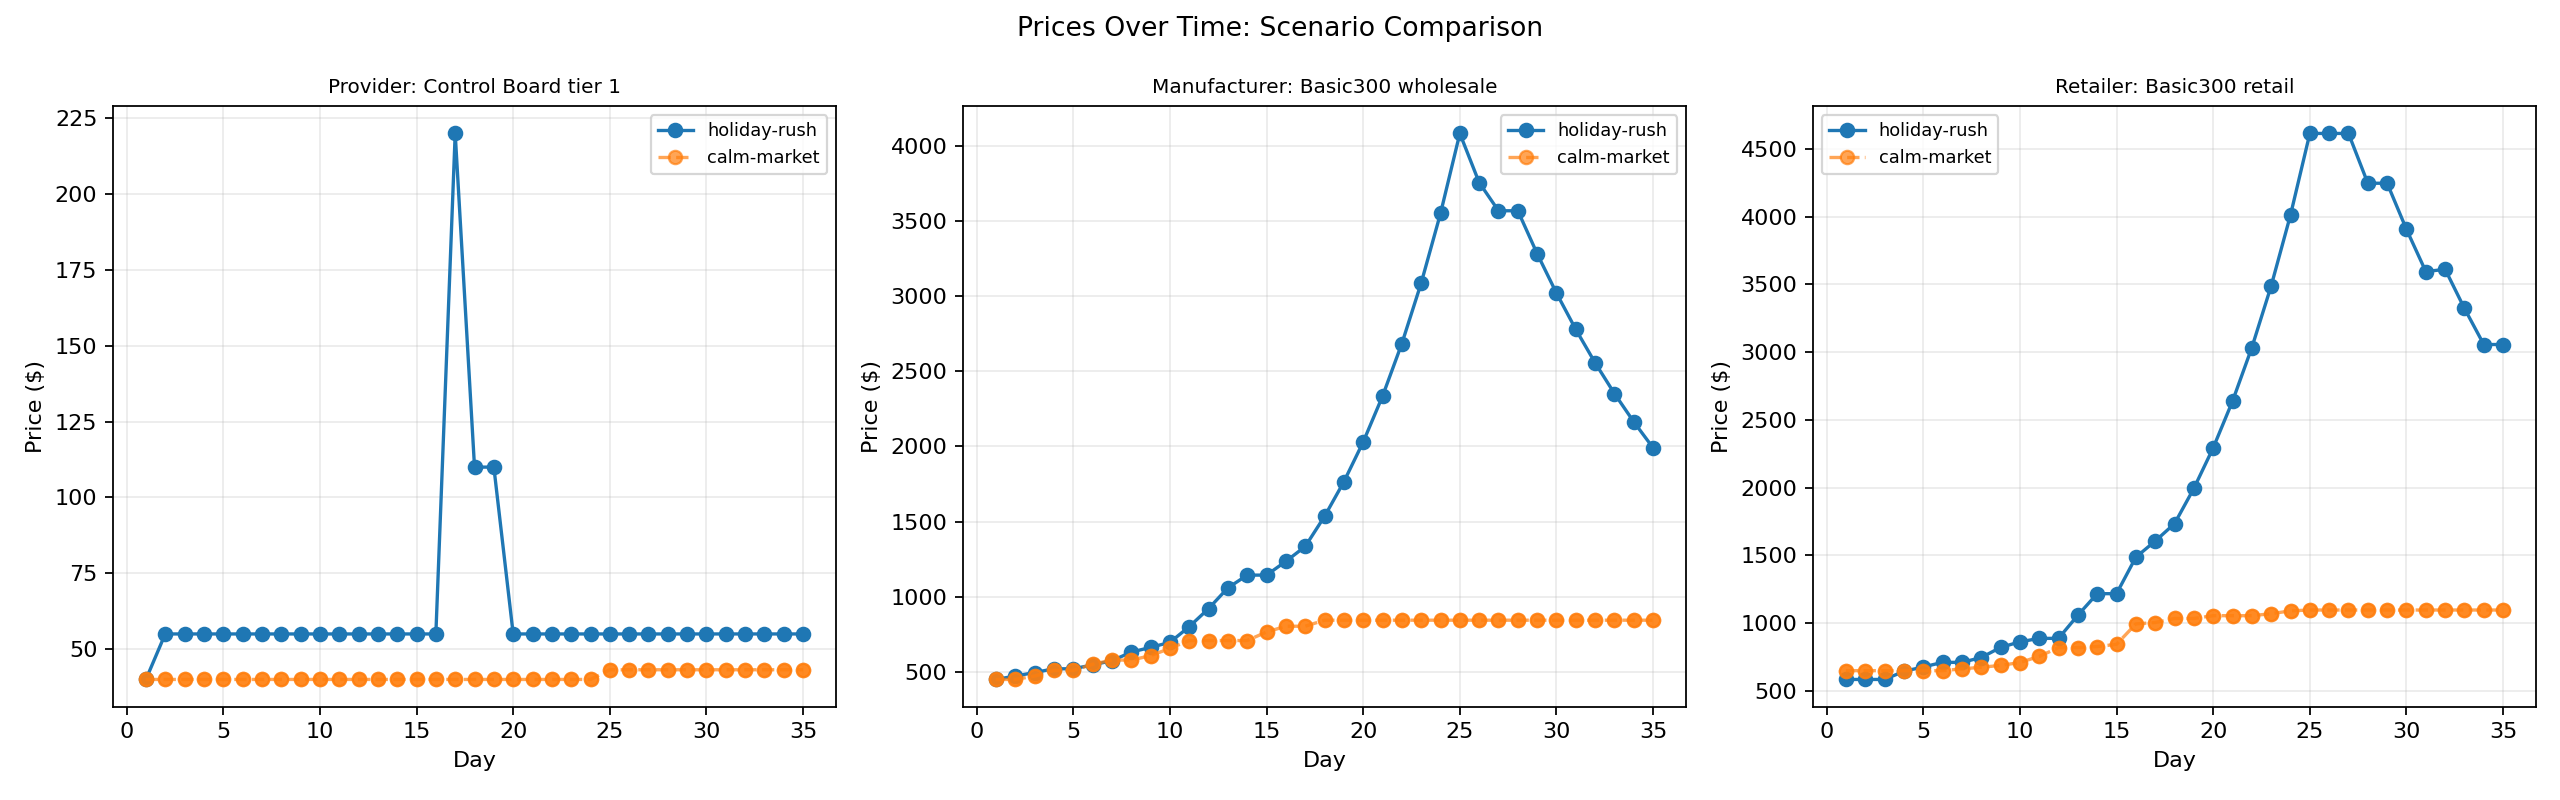
\includegraphics[width=0.9\textwidth]{images/comparison_prices_over_time.png}
\caption{Printer prices: holiday-rush vs calm-market}
\end{figure}

\begin{figure}[H]
\centering
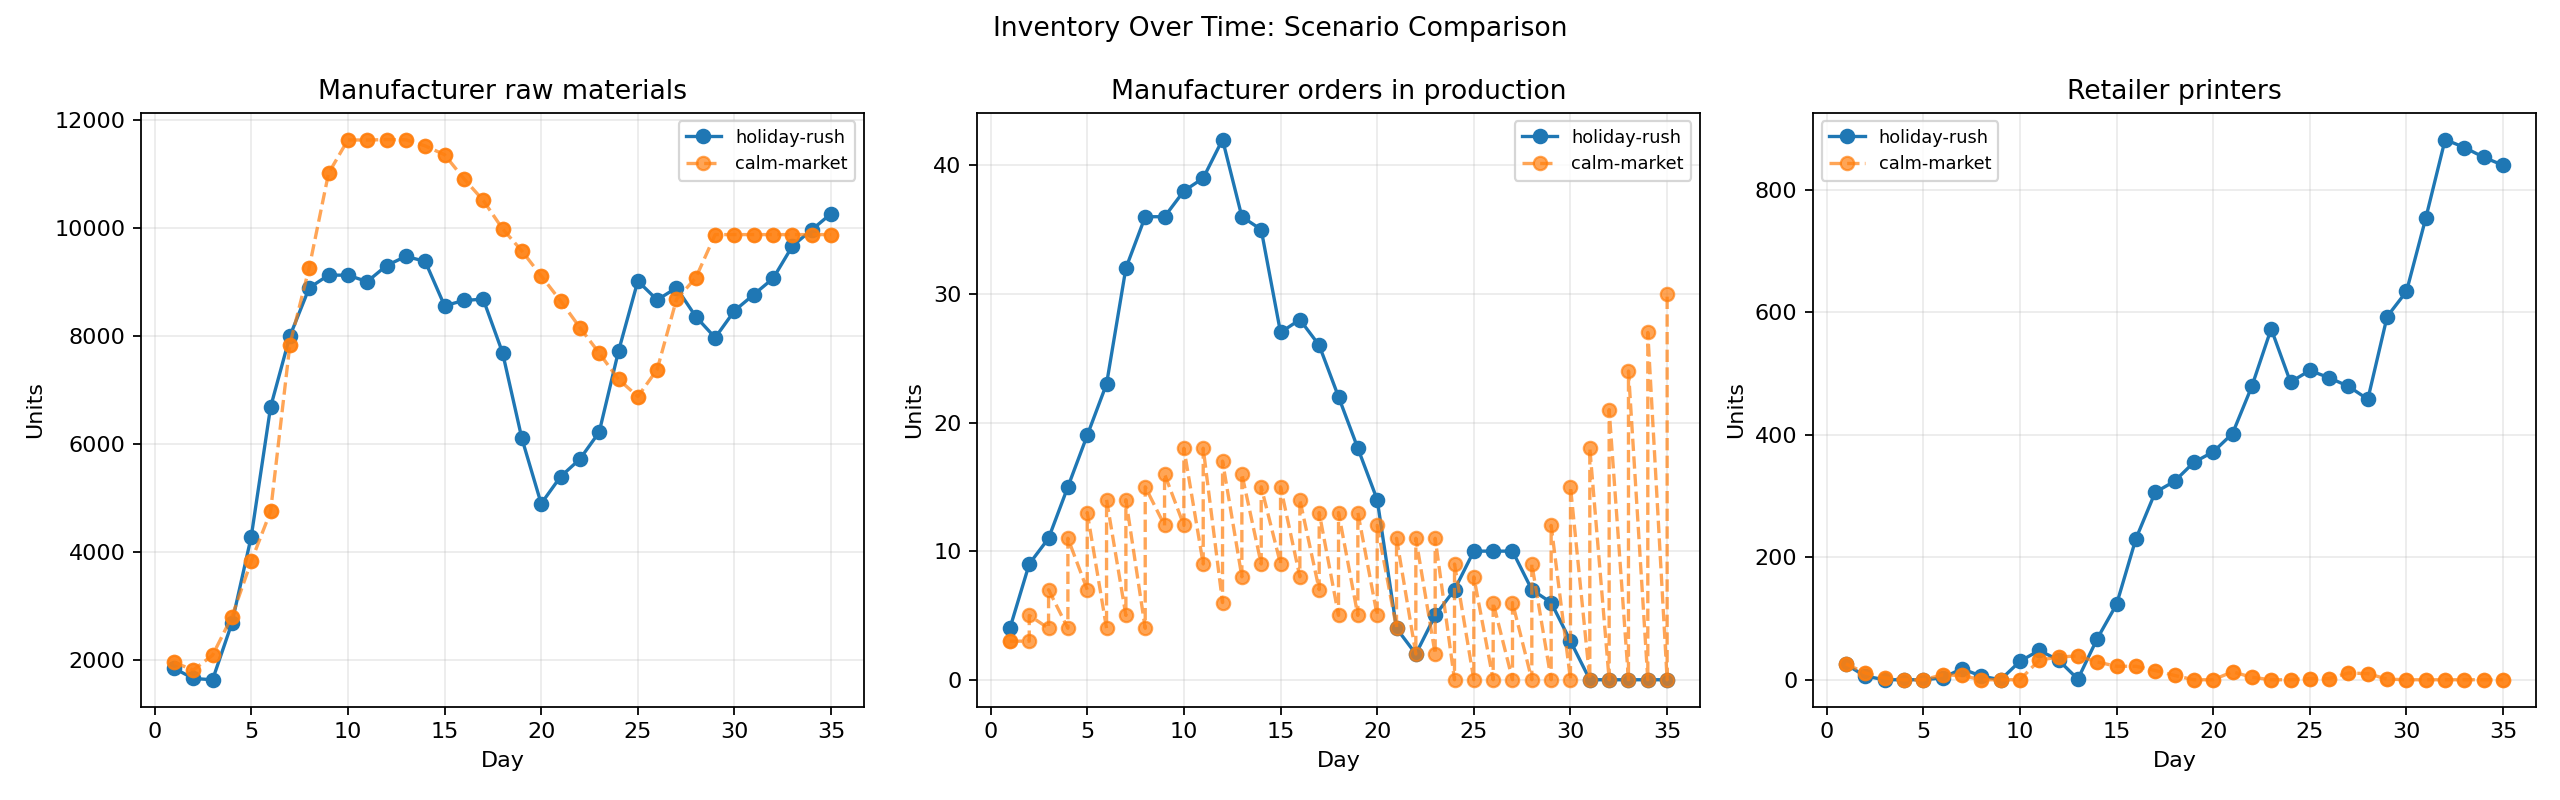
\includegraphics[width=0.9\textwidth]{images/comparison_inventory_over_time.png}
\caption{Retailer \& manufacturer inventory: holiday-rush vs calm-market}
\end{figure}

\begin{figure}[H]
\centering
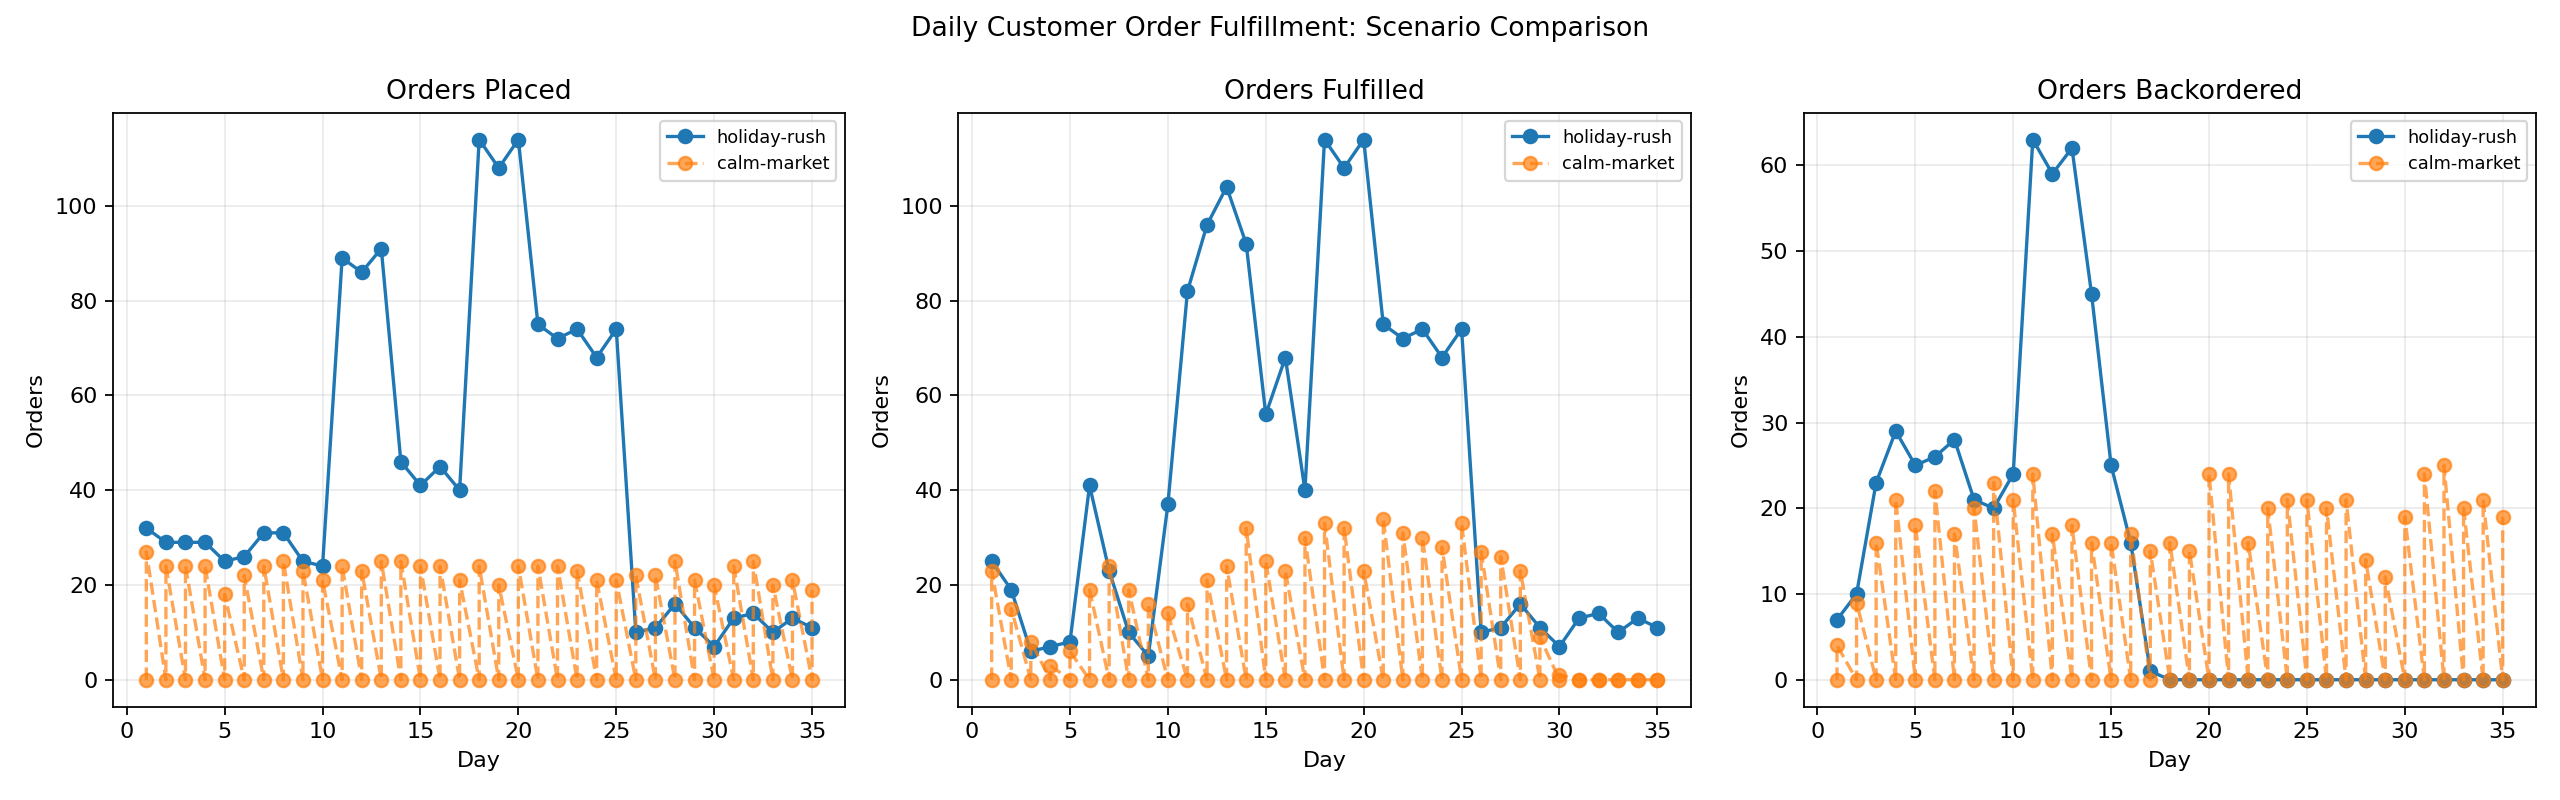
\includegraphics[width=0.9\textwidth]{images/comparison_order_fulfillment.png}
\caption{Order fulfillment: holiday-rush vs calm-market}
\end{figure}

\begin{itemize}
\tightlist
\item
  \textbf{Prices:} The holiday run produced a 9× wholesale price swing
  (450 → 4,082 → 1,990) driven by the demand surges. The calm run barely
  moved, peaking at 844 on day 20, less than double the starting price.
\item
  \textbf{Buffer-building:} In the holiday run, demand spikes triggered
  proactive inventory build-up; the retailer reached 48 printers ahead
  of Black Friday and 840 by the end. In the calm run, the retailer's
  stock never recovered from the day 3--10 stockout and stayed near zero
  for most of the simulation.
\item
  \textbf{Backorders:} Counterintuitively, the volatile run produced
  fewer total backorders (484 vs 646), because the agents responded
  better to change than to a flat steady-state signal. The demand
  spikes prompted action that the calm signal did not.
\item
  \textbf{Assembly lines:} Neither scenario triggered the manufacturer
  to open more than 2 lines, suggesting the scaling thresholds were
  conservative enough that a 35-day holiday surge did not cross them.
\item
  \textbf{Failure modes:} Opposite outcomes from the same agents, the
  holiday run ended in post-holiday overstock with no mechanism to clear
  it; the calm run ended in chronic understocking with no mechanism to
  build up. Both are failures of adaptation, just in opposite
  directions.
\end{itemize}



\subsection{Emergent Behaviour}\label{emergent-behaviour}

The most surprising behaviour was ``stress-induced perfect fulfillment''
on days 18--20, the hardest window in the entire simulation. The chip
shortage (supply\_modifier = 0.4) and Christmas rush (demand\_modifier
up to 3.75 combined) overlapped simultaneously, yet those three days
recorded 114/108/114 orders placed and 114/108/114 fulfilled: 100\%
fulfillment with zero backorders. Every other stressed period produced
backorders. What happened is that the chip shortage had already forced
the manufacturer to build up a large inventory buffer during days 14--17
(when demand was only 1.5×), and that buffer was exactly what the system
needed when demand tripled. The agents did not plan this, they each
followed their independent skill rules, but the timing of the two events
created an accidental alignment between inventory peaks and demand peaks
that neither a pure demand surge nor a pure supply shock would have
produced alone.

A second emergent behaviour was model-dependent: the same skill file
produced opposite outcomes depending on which LLM ran it. In the Gemini
run on a calm-market scenario, the manufacturing agent opened 8 assembly
lines despite zero backlog, zero demand surge, and no pending orders,
burning \$13,600/day with zero output and finishing at $-$\$859,397 net
loss. The Claude/Haiku run on the identical skill file stayed at 2 lines
throughout. The instruction was ambiguous enough that Gemini misread it;
Claude followed it correctly. This was not a bug in the skill file in
any absolute sense, it was an emergent property of how different models
interpret the same natural-language instruction differently, and the
only way to discover it was to run the full simulation with each model.



\section{Vibe-Coding Reflection}\label{d-vibe-coding-reflection}

\subsection{How we used Claude Code}\label{how-we-used-claude-code}

Claude Code was used at different layers in Week 8: it wrote the turn
engine scaffolding, generated the initial skill files, and was then used
iteratively to refine those skills as failure modes appeared in logs.
Week 8 prompts were observation-driven (``the agent wrote this in the
log, why is it wrong and how do we fix the skill?''). Claude Code was
also used to generate graphs from \texttt{metrics.jsonl}.

\subsection{What worked}\label{what-worked}

The same pattern that worked in Week 6 held in Week 8: precise,
file-scoped prompts with explicit PRD section references produced
correct code on the first attempt. Asking Claude Code to implement a
named function in a named file, with numbered acceptance criteria,
eliminated most ambiguity.

The skill files themselves benefited from an iterative loop: run one day
in isolation, read the log, identify a bad decision, tighten the skill,
repeat.

\subsection{What did not work}\label{what-did-not-work}

Skill ambiguities cannot be caught by reading the file, they only
surface when the simulation runs and the agent logs its own reasoning.
The clearest example was the ``empty queue means no capacity''
misreading: the manufacturing skill said to check the queue before
releasing orders, which looks correct on paper, but the agent read an
empty queue as ``nothing to produce'' rather than ``the factory is idle,
release now.'' This caused it to sit idle on days 6 and 8 with pending
orders it could have filled. A related gap was the missing downscaling
rule: the skill had clear instructions for opening assembly lines but
none for closing them, so the agent kept paying fixed line costs through
the final days of the run despite producing nothing and the retailer
already holding 840 printers in stock.

\subsection{The one thing we would
redesign}\label{the-one-thing-we-would-redesign}

The sequential turn order (provider, then manufacturer, then retailer)
is the single design decision we would change. Each agent acts on
yesterday's state and can never react to the same-day decisions of the
agents that went before it: the manufacturer ships to the retailer
before the retailer has placed that day's demand, and the provider
confirms delivery before the manufacturer has processed it. This lag is
what produced the days 3--6 stockout cascade: even though the
manufacturer had stock on day 3, the retailer's replenishment order
placed on day 2 could not be fulfilled until the next turn. A
synchronous round model, where all three agents propose actions, then a
resolver applies them in a single atomic step, would eliminate the
one-day propagation delay and more accurately reflect how a real supply
chain negotiates the same business day.

\appendix

\begin{landscape}
\section{System Architecture Diagram}
\label{appendix:architecture}
\vspace{1cm}
\begin{figure}[h]
\centering

\includegraphics[width=\linewidth]{images/grafico.png}
\caption{Full system architecture: Turn Engine, Provider (ChipSupply Co), Manufacturer (Factory), and Retailer (PrinterWorld).}
\end{figure}
\end{landscape}

\end{document}
